\documentclass[
% reprint,
%preprint, 
% 11pt,
% 10pt,
%superscriptaddress,
%groupedaddress,
%unsortedaddress,
%runinaddress,
% frontmatterverbose, 
%preprintnumbers,
%nofootinbib,
%nobibnotes,
%bibnotes,
aps,
pra,
% linenumbers,
twocolumn,
% prl,
% prb,
% prd,
% rmp,
% prstab,
% prstper,
floatfix,
%longbibliography
]{revtex4-2} 
% \usepackage{revquantum}
% new linux font, ignore mono
% \usepackage[mono=false]{libertine} 
% \renewcommand{\baselinestretch}{1.05}
% \usepackage[top=0.7in,left=1in,bottom=1in,right=1in]{geometry}
\usepackage{amsmath,amsthm,amssymb,epsfig,graphicx,mathrsfs,amsfonts,dsfont,bbm}
% \usepackage{bbm} % for \mathbb{1}, but ruins the letter
% \usepackage{unicode-math}
% \DeclareMathOperator*{\argmax}{argmax}
% \DeclareMathOperator*{\argmin}{argmin}
\usepackage{pict2e}
\usepackage[percent]{overpic}
\usepackage{color}
\usepackage{listings}
\usepackage{caption}
% \usepackage{fullpage}
\usepackage[toc,title,titletoc,header]{appendix}
\usepackage{color}
\usepackage{dcolumn}
\usepackage{bm}
\usepackage{hyperref}
\hypersetup{
    citecolor=magenta,
    colorlinks=true,
    linkcolor=blue,
    filecolor=green,      
    urlcolor=cyan,
}
\usepackage[capitalise]{cleveref}
\usepackage{subcaption}
\usepackage{enumitem}
\setlist[enumerate]{leftmargin=10mm, label=\alph*)}
\setlist[itemize]{leftmargin=12pt}
\usepackage{mathtools}
\usepackage{tikz}
\usepackage{tkz-graph} % graph theory
%\usepackage{tikzit}
%\input{path_integral.tikzstyles}
\usepackage{braket}
\usepackage{physics}
% \usepackage{luatex85} % for qcircuit
\usepackage{luatex85,qcircuit}
\usepackage{blkarray}
\usepackage[linesnumbered,ruled,vlined,algosection]{algorithm2e}
\newcommand\mycommfont[1]{\footnotesize\ttfamily\textcolor{blue}{#1}}
\SetCommentSty{mycommfont}

% \setlength\parindent{0pt}
\setcounter{secnumdepth}{3}

\theoremstyle{plain}
\newtheorem{axiom}{Axiom}
\newtheorem{theorem}{Theorem}
\newtheorem{corollary}{Corollary}
\newtheorem{lemma}{Lemma}
\newtheorem{proposition}{Proposition}
\newtheorem{conjecture}{Conjecture} 
\newtheorem{question}{Question} 
\newtheorem{claim}{Claim} 

\theoremstyle{definition}
\newtheorem{definition}{Definition}
\newtheorem*{problem*}{Problem} 
\newtheorem{problem}{Problem}
\newtheorem{notation}{Notation}
\newtheorem{observation}{Observation} 
\newtheorem{fact}{Fact}
\newtheorem{example}{Example}
\newtheorem{remark}{Remark}


% !TEX root = ./notes.tex

%%%%%%%%%%%%%%%%%%%%%%%%%%%%%%%%%%%%
%%%%%%%%%%%%%% math %%%%%%%%%%%%%%%%
%%%%%%%%%%%%%%%%%%%%%%%%%%%%%%%%%%%%
\newcommand{\calH}{\mathcal{calH}}
\newcommand{\hilbertspace}{\mathcal{H}}
\newcommand{\bigO}{\mathcal{O}}
\newcommand{\lagrangian}{\mathcal{L}}
\newcommand{\VS}{\textrm{VS}}

\newcommand{\realnumber}{\mathbb{R}}
\newcommand{\complexnumber}{\mathbb{C}}
\newcommand{\rationalnumber}{\mathbb{Q}}
\newcommand{\integer}{\mathbb{Z}}
\newcommand{\naturalnumber}{\mathbb{N}}
\newcommand{\numberfield}{\mathbb{F}}

\newcommand{\0}{\mathbf{0}}
\newcommand{\bI}{\mathbf{I}}
\newcommand{\identity}{\mathds{1}}
\newcommand{\midentity}{\mathds{1}}
% \newcommand{\identity}{\mathbb{1}}
\newcommand{\bX}{\mathbf{X}}
\newcommand{\bY}{\mathbf{Y}}
\newcommand{\bepsilon}{\boldsymbol{\epsilon}}

\newcommand{\ii}{\textup{i}}

\newcommand{\floor}[1]{\left\lfloor #1 \right\rfloor}
\newcommand{\ceil}[1]{\left\lceil #1 \right\rceil}

% probability
\newcommand{\probability}{\mathbb{P}}
\newcommand{\variance}{\textup{\textrm{Var}}}
\newcommand{\covariance}{\textup{\textrm{Cov}}}
\newcommand{\expectation}{\mathbb{E}}

% group theory
\newcommand{\group}{\mathbb{G}}
\newcommand{\dihedral}{\mathbb{D}}
\newcommand{\GL}{\mathbb{GL}}
\newcommand{\SL}{\mathbb{SL}}
\newcommand{\Sp}{\textup{Sp}}
% \newcommand{\sp}{\mathfrak{sp}}
\newcommand{\SU}[1]{\textup{SU(#1)}}
\newcommand{\su}[1]{\mathfrak{su}(#1)}
% \renewcommand{\SO}[1]{\textup{SO(#1)}}
% \newcommand{\SO}{\textup{SO}}

% graph theory
\newcommand{\graph}{G}

% matrix and linear algebra
\newcommand{\diag}{\textup{diag}}
% \let\span\relax
% \DeclareMathOperator{\span}{\textup{span}}
% \newcommand{\span}{\textup{span}}
\newcommand{\spn}{\mathop{\mathrm{span}}}
\DeclareMathOperator{\spann}{\textup{span}}
%%%%%%%%%%%%%%%%%%%%%%%%%%%%%%%%%%%%
%%%%%%%%%%%%%%  CS  %%%%%%%%%%%%%%%%
%%%%%%%%%%%%%%%%%%%%%%%%%%%%%%%%%%%%
% cryptography
\newcommand{\gen}{\textsf{Gen}}
\newcommand{\enc}{\textsf{Enc}}
\newcommand{\dec}{\textsf{Dec}}
\newcommand{\mac}{\textsf{Mac}}
\newcommand{\sign}{\textsf{Sign}}
\newcommand{\verfy}{\textsf{Verfy}}
\newcommand{\negl}{\textup{negl}}

% quantum computing
% gates
\newcommand{\cnot}{\textup{\textsc{cnot}}}
\newcommand{\hdm}{\textup{\textsc{h}}}
\newcommand{\tphase}{\textup{\textsc{t}}}
\newcommand{\cphase}{\textup{\textsc{cphase}}}
\newcommand{\swap}{\textup{\textsc{swap}}}
\newcommand{\negate}{\textup{\textsc{not}}}
\newcommand{\QFT}{\textup{QFT}}

% Boolean Functions
\newcommand{\MAJ}{\textup{\textsc{maj}}}
\newcommand{\NOT}{\textup{\textsc{not}}}
\newcommand{\OR}{\textup{\textsc{or}}}
\newcommand{\AND}{\textup{\textsc{and}}}
\newcommand{\NAND}{\textup{\textsc{nand}}}
\newcommand{\EQ}{\textup{\textsc{eq}}}
\newcommand{\IP}{\textup{\textsc{ip}}}
\newcommand{\DISJ}{\textup{\textsc{disj}}}
\newcommand{\Parity}{\textup{\textsc{parity}}}
\newcommand{\Threshold}{\textup{\textsc{thr}}}

\newcommand{\GS}{\textup{\textsc{gs}}}
\newcommand{\dejo}{\textup{\textsc{DeJo}}}
\newcommand{\STAB}{\textup{\textsc{stab}}}

% algorithms
\newcommand{\algo}{\mathcal{A}}
\newcommand{\maxcut}{\textup{\textsc{MaxCut}}}
\newcommand{\sat}{\textup{\textsc{sat}}}
\newcommand{\partition}{\textup{\textsc{Partition}}}
\newcommand{\bosonsample}{\textup{\textsc{BosonSampling}}}

% complexity measures
\newcommand{\vcdim}{\mathsf{VCdim}}
\DeclareMathOperator{\certificate}{\mathsf{Cert}}
\DeclareMathOperator{\s}{\mathsf{s}}
\DeclareMathOperator{\bs}{\mathsf{bs}}
\DeclareMathOperator{\adeg}{\mathsf{\widetilde{deg}}}
% \DeclareMathOperator{\adv}{\mathsf{Adv}}
\DeclareMathOperator{\dqc}{\mathsf{D}}
\DeclareMathOperator{\rqc}{\mathsf{R}}
\DeclareMathOperator{\qqc}{\mathsf{Q}}
\DeclareMathOperator{\cmc}{\mathsf{C}}
\DeclareMathOperator{\rcmc}{\mathsf{RC}}
\DeclareMathOperator{\qcmc}{\mathsf{QC}}
\let\deg\relax
\DeclareMathOperator{\deg}{\mathsf{deg}}
\DeclareMathOperator{\poly}{\textup{poly}}

% complexity classes
\newcommand{\reduceto}{\le_P}
\let\cclass\textup
\let\P\relax
\newcommand{\P}{\cclass{P}}
\newcommand{\PP}{\cclass{PP}}
\newcommand{\NP}{\cclass{NP}}
\newcommand{\sharpP}{\cclass{\#P}}
\newcommand{\coNP}{\cclass{co-NP}}
\newcommand{\PH}{\cclass{PH}}
\newcommand{\NPC}{\cclass{NPC}}
\newcommand{\BQP}{\cclass{BQP}}
\newcommand{\QMA}{\cclass{QMA}}
\newcommand{\PSPACE}{\cclass{PSPACE}}
\newcommand{\BPP}{\cclass{BPP}}

% Optimization
\newcommand{\subjectto}{\textup{subject to  }}

\let\iff\relax
\newcommand{\iff}{\text{ iff }}
\newcommand{\eff}{\textup{eff}}
\newcommand{\st}{\text{ s.t. }}
\newcommand{\otherwise}{\text{otherwise}}
\newcommand{\T}{\intercal}
\newcommand{\OPT}{\textup{OPT}}


\newcommand\vartextvisiblespace[1][.5em]{%
  \makebox[#1]{%
    \kern.07em
    \vrule height.3ex
    \hrulefill
    \vrule height.3ex
    \kern.07em
  }% <-- don't forget this one!
}
\newcommand{\visiblespace}{\vartextvisiblespace}

%%%%%%%%%%%%%%%%%%%%%%%%%%%%%%%%%%%%
%%%%%%%%%%%%% Physics %%%%%%%%%%%%%%
%%%%%%%%%%%%%%%%%%%%%%%%%%%%%%%%%%%%
\newcommand{\zpartition}{\mathcal{Z}}
\newcommand{\llaplacian}{\mathfrak{L}}
\newcommand{\dlagrangian}{\mathcal{L}}
\newcommand{\eaction}{\mathcal{A}}
\newcommand{\action}{\mathcal{S}}
\newcommand{\hhat}{\hat{H}}
\newcommand{\xhat}{\hat{x}}
\newcommand{\phat}{\hat{p}}
\newcommand{\qhat}{\hat{q}}
\newcommand{\nhat}{\hat{n}}
\newcommand{\pihat}{\hat{\pi}}
\newcommand{\phihat}{\hat{\phi}}
\newcommand{\oph}{\mathbf{H}}
\newcommand{\opx}{\mathbf{x}}
\newcommand{\opp}{\mathbf{p}}
\newcommand{\opq}{\mathbf{q}}
\newcommand{\vecx}{\vec{x}}
\newcommand{\vecp}{\vec{p}}
\newcommand{\veck}{\vec{k}}
\newcommand{\vecq}{\vec{q}}
\newcommand{\vbk}{\vb{k}}
\newcommand{\vbs}{\vb{s}}
\newcommand{\vbx}{\vb{x}}
\newcommand{\vbn}{\vb{n}}
\newcommand{\vbp}{\vb{p}}
\newcommand{\vbq}{\vb{q}}
\newcommand{\vbr}{\vb{r}}
\newcommand{\vbe}{\vb{e}}
\newcommand{\vbv}{\vb{v}}
\newcommand{\vbw}{\vb{w}}
\newcommand{\vbB}{\vb{B}}
\newcommand{\vbE}{\vb{E}}
% \newcommand{\acreation}{\hat{a}^\dagger}
% \newcommand{\aannihilation}{\hat{a}}
\newcommand{\acreation}{\hat{a}^\dagger}
\newcommand{\aannihilation}{\hat{a}}
\newcommand{\bcreation}{\hat{b}^\dagger}
\newcommand{\bannihilation}{\hat{b}}
\newcommand{\ccreation}{\hat{c}^\dagger}
\newcommand{\cannihilation}{\hat{c}}
\newcommand{\homega}{\hbar \omega}
\newcommand{\opsigma}{\hat{\bm{\sigma}}}
\newcommand{\hatsigma}{\hat{\sigma}}
\newcommand{\bmhsig}{\bm{\hat{\sigma}}}
\newcommand{\hsig}{\hat{\sigma}}
\newcommand{\si}{\hat{\sigma}_0}
\newcommand{\sx}{\hat{\sigma}_x}
\newcommand{\sy}{\hat{\sigma}_y}
\newcommand{\sz}{\hat{\sigma}_z}
\newcommand{\splus}{\hat{\sigma}_+}
\newcommand{\sminus}{\hat{\sigma}_-}
\newcommand{\px}{\hat{X}}
\newcommand{\py}{\hat{Y}}
\newcommand{\pz}{\hat{Z}}
\newcommand{\pI}{\hat{I}}
\newcommand{\schrodinger}{\textup{Schr\"{o}dinger }}
\newcommand{\tc}{T_c}
\newcommand{\alembertian}{\square}
\newcommand{\vecA}{\vb{A}}
\newcommand{\magfield}{\vb{B}}
\newcommand{\elefield}{\vb{E}}

\newcommand{\deltat}{\Delta t}
\newcommand{\deltatau}{\Delta \tau}

%%%%%%%%%%%%%%%%%%%%%%%%%%%%%%%%%%%%
%%%%%%%%%%%%% Quantum Computing %%%%%%%%%%%%%%
%%%%%%%%%%%%%%%%%%%%%%%%%%%%%%%%%%%%
% \newcommand{\gcommutator}[1]{[[ #1 ]]}
\usepackage{stmaryrd}
\newcommand{\gcommutator}[1]{\llbracket #1 \rrbracket}
\newcommand{\kernel}{k}
\newcommand{\ew}{W}
\newcommand{\ob}{O}
\newcommand{\pob}{O}
\newcommand{\dm}{\rho}
% \newcommand{\ob}{\hat{O}}
% \newcommand{\ew}{\hat{W}}
\newcommand{\ghz}{\text{GHZ}}
\newcommand{\jsd}{\text{JS}}
\newcommand{\qjs}{\text{QJS}}
\newcommand{\kl}{\text{KL}}
\newcommand{\ml}{\text{ml}}
\newcommand{\bi}{\text{bi}}
\newcommand{\cs}{\text{cs}}
\newcommand{\svm}{\text{svm}}
\newcommand{\shadow}{\textup{shadow}}
\newcommand{\ansatz}{\textup{ansatz}}
\newcommand{\tomo}{\textup{tomo}}
\newcommand{\target}{\textup{tar}}
\newcommand{\prepare}{\textup{pre}}
\newcommand{\entangled}{\textsf{entangled}}
\newcommand{\noise}{\text{noise}}
\newcommand{\qnn}{\textup{QNN}}
\newcommand{\ntk}{\textup{NT}}
\newcommand{\ppt}{\textup{PPT}}
\newcommand{\bells}{\textup{BELL}}
\newcommand{\chsh}{\textup{CHSH}}
\newcommand{\bellineq}{\textup{Bell}}
\newcommand{\locc}{\textup{LOCC}}
% \newcommand{\ml}{\textup{ml}}
\newcommand{\stbz}{\hat{S}}
\newcommand{\separable}{\mathcal{S}}
\newcommand{\si}{\hat{\sigma}_0}
\newcommand{\sx}{\hat{\sigma}_x}
\newcommand{\sy}{\hat{\sigma}_y}
\newcommand{\sz}{\hat{\sigma}_z}
\newcommand{\px}{X}
\newcommand{\py}{Y}
\newcommand{\pz}{Z}
\newcommand{\pI}{I}
\newcommand{\bmsigma}{\bm{\sigma}}

\renewcommand{\llaplacian}{\hat{\mathfrak{L}}}
%\newcommand{\zpartition}{\mathcal{Z}}
\newcommand{\hamiltonian}{\hat{H}}
\newcommand{\U}{U}
% \newcommand{\U}{\hat{U}}
\newcommand{\subgroup}{\mathbb{H}}
\newcommand{\ppartition}{\mathcal{P}}
\newcommand{\oracle}{\hat{O}}
\newcommand{\D}{\mathcal{D}}
\newcommand{\proj}{\hat{P}}
%\newcommand{\deltat}{\Delta t}
%\newcommand{\deltatau}{\Delta \tau}
\newcommand{\cz}{\textup{\textsc{cz}}}
\newcommand{\cx}{\textup{\textsc{cx}}}
\newcommand{\toffoli}{\textup{\textsc{toffoli}}}
\newcommand{\lleft}{\leftarrow}
\newcommand{\rright}{\rightarrow}
\newcommand{\intinf}{\int_{-\infty}^{\infty}}

% disable subsections and subsubsections in the TOC
\makeatletter
%\def\l@subsection#1#2{}
\def\l@subsubsection#1#2{}
\makeatother

\begin{document}
%%%%%%%%%%%%%%%%%%%
\title{Towards efficient and generic entanglement detection}
\author{Jue Xu}
\email{juexu@cs.umd.edu}
\author{Qi Zhao}
\email{zhaoqi@cs.hku.hk}
% \affiliation{Department of Computer Science, University of Maryland, College Park.}
\date{\today}
%%%%%%%%%%%%%%%%%%%
\begin{abstract}
	Detection of entanglement is an indispensable step to practical quantum computation and communication.
	In this work, we propose an end-to-end, machine learning assisted entanglement detection protocol.
	In this protocol, an entanglment witness for a generic entangled state is obtained by classical machine learning with a synthetic dataset which consists of classical features of states and their labels. 
	In actual experiments, classical features of a state, that is expectation values of a set of  Pauli observables, are estimated by sample-efficient methods such as classical shadow.
	% In this work, we compare complexity and performance of several recently-developed methods, including entanglement witness methods, shadow tomography, classical machine learning, and quantum algorithms (circuits).
	% We illustrate the advantages and limitations of machine learning and quantum algorithms.
\end{abstract}

\maketitle
% \setcounter{tocdepth}{0}
% \tableofcontents

%%%%%%%%%%%%%%%Content%%%%%%%%%%%%%%%
\section{Introduction}
Entanglement \cite{horodeckiQuantumEntanglement2009} is the key ingredient of quantum computation \cite{briegelMeasurementbasedQuantumComputation2009}, quantum communication, and quantum cryptography \cite{xuSecureQuantumKey2020}.
% Entanglement is the key property of quantum mechanics which makes it fundamentally different from the classical world. With entanglement, quantum computers can significantly outperform their classical counterparts. On the other hand, entanglement provides more secure communication and encryption schemes. 
However, decoherence is inevitable in real-world, which means the interaction between a quantum system and classical environment would significantly affect entanglement quality and diminish quantum advantage. 
So, for practical purpose, it is essential to benchmark (characterize) entanglement structures of certain target states in actual (real) experiments.
The goal of this paper is to find an efficient and generic way to achieve it. 
Machine learning (ML) is a powerful tool for such purpose. 
Many ML techniques including quantum machine learning models \cite{congQuantumConvolutionalNeural2019} have been proposed for classification tasks in physics, such as classification of phases and prediction of ground states \cite{carrasquillaMachineLearningPhases2017} \cite{huangProvablyEfficientMachine2022}.
% There are quantum machine learning algorithms for quantum problems (data) 

% Roughly, our solution is to make use of both machine learning techniques and some recently-developed quantum algorithms.
Assume we would like to distinguish an entangled state incluing its `vicinity' (proximity) from undesired states (e.g., all separable states), our method derive such a classifier by fitting a synthetic dataset randomly sampled states with their labels ($\entangled$ or not).
Specifically, our pipeline starts from evaluation of expectations of $n$-qubit Pauli observables of a target state. 
The set of expectation values that serves as classical features of the target state, together with its label, consist of a data point of a dataset.
Then, a classical ML classifier is obtained by training with this dataset.
% non-linear kernels, which can be viewed as a non-linear entanglement witness. 
% Probably, we can eliminate unimportant features, which means we might not need all pauli operators in our generic witness. 
With the trained classifier at hand, it is expected that brand new samples from real experiments can be classified with high accuracy, 
where classical features of quantum states are estimated by classical shadow method \cite{huangPredictingManyProperties2020} with affordable samples complexity.

This paper is organized as follows: in \cref{sec:preliminaries}, we briefly present necessary definitions about entanglement structures and mainstream entanglement detection methods;
\cref{sec:protocol} demonstrates our end-to-end protocol including two parts: learning an entanglement witness from synthetic data and estimating classical features of states from experiments;
at last, numerical simulation results are discussed in \cref{sec:numerical_simulation}.

\section{Preliminaries}\label{sec:preliminaries}
% \subsection{Related works}
% \subsection{Notations}
% Notations: 
% \begin{notation}
% 	The hats on the matrices such as
% 	% $\hat{A}$, Hamiltonian $\hamiltonian$, 
% 	observables $\ob$, entanglement witness $\ew$, 
% 	emphasize that they play the roles of operators (Hermitian matrices).
% 	density matrix $\dm$ (omitted)
% 	$\qty{I,X,Y,Z}$
% \end{notation}

% \begin{notation}
% 	In machine learning setting,
% 	denote vector (matrix) $\vbx$, $\vbw$, $\vb{K}$ by boldface font.
% 	% A simle (undirected, unweighted) graph $\graph=(V,E)$ is described by vertices $V$ and edges $E$.
% \end{notation}

% For specific purpose, we use different basis (representations) for quantum states.
% One is the computational basis $\qty{\ket{z}}$ with $z\in \qty[2^n]$ where $n$ is the number of qubits,
% while another useful one is the binary representation of computational basis $\qty{\ket{\vbx}\equiv\ket{x_1}\ket{x_2}\dots\ket{x_n}}$ with $x_j\in \qty{0,1}$. 
% For simplicity, we let $N \equiv 2^n$ and $\ket{\vb{0}}\equiv\ket{0^n} \equiv\ket{0}^{\otimes n}$ if no ambiguity.
\begin{notation}
	If no ambiguity,
	we omit the tensor products between subsystems and the hats on operators for readability,
	e.g.,
	% shorthand 
	$\ket{\psi_A}\ket{\psi_B}\equiv \ket{\psi_A}\otimes \ket{\psi_B}$ 
	% Hadamard basis $\ket{+}: = (\ket{0}+\ket{1})/\sqrt{2} $.
	and $\px^{(1)}\pz^{(3)} \equiv \hat{X} \otimes \identity \otimes \hat{Z}$.
\end{notation}
\begin{notation}
	Denote $\pob_{\sigma}\in \qty{I,X,Y,Z}^{\otimes n}$ for a Pauli observable.
	% Denote $\pob_{\sigma}:=\bigotimes \sigma$ for a Pauli observable.
	% where $\sigma\in \qty{I,X,Y,Z}^n$ is a string of Pauli operators.
	Denote $\vbx_{\dm,\bmsigma}:=(\Tr(\dm\pob_{\sigma_1}),\dots,\Tr(\dm\pob_{\sigma_M}))$ for expectations of $M$ Pauli observables with respect to the state $\dm$ where $\bmsigma\subseteq \qty{I,X,Y,Z}^n$.
	Denote vectors $\vbx$, $\bmsigma$, $\vbw$ by boldface font.
\end{notation}
% \begin{notation}
% 	% $d$ for $d$-dimensional qudit; 
% 	$D\equiv d^n$ as the dimension of a $n$-qudit systems.
% \end{notation}

\subsection{Entanglement structures}
% \subsection{Entanglement detection}

% \subsubsection{Bipartite entanglement}
Large scale entanglement involving multiple particles maybe the main resource for quantum advantages in quantum computation and communication.
Roughly, we say a quantum state is \emph{entangled} if it is not fully separable,
i.e., the state cannot be written as the tensor product of all subsystems.
% \begin{definition}[fully separable]\label{def:fully_separable}
% 	An $n$-particle (qubit) pure state $\ket{\psi_f}$ is fully separable 
% 	if it can be written as the tensor product of all subsystems $\qty{A_1,\dots,A_n}$, i.e., $\ket{\psi_f}=\bigotimes_{i=1}^n \ket{\phi_{A_i}}$.
% 	% Analoguous to \cref{eq:mixed}, 
% 	Analoguously, a mixed state $\dm_f$  is fully separable if it can be written as a convex combination of fully separable pure states.
% 	% (, and is (fully) $n$-separable if it is in $S_n$).
% 	% An $n$-qubit pure state $\ket{\psi_f}$ is $\ppartition$-fully separable $\iff$ it can be written as 
% 	% $\ket{\psi_f}=\otimes_i^m \ket{\phi_{A_i}}$.
% 	% Analoguous to \cref{eq:mixed}, an $n$-qubit mixed state $\dm_f$ is $\ppartition$-fully separable $\iff$ it can be decomposed into a convex mixture of $\ppartition$-fully separable pure states.
% 	% % \begin{equation}
% 	% % 	\dm_f = \sum_i p_i \op{\psi_f^i}, (\forall i) ( p_i\ge 0, \sum_i p_i = 1) .
% 	% % \end{equation}
% 	% P-bi-separable... $\separable_f^\ppartition \subset S_b^\ppartition$
% \end{definition}
However, the simple statement `the state is entangled' would allow that only two of the particles are entangled while the rest is in a product state.
So, the more interesting entanglement property is bipartite separability.
Consider a system partitioned into two subsystems $\hilbertspace_A \otimes \hilbertspace_B$, where each has dimension $d_A$ and $d_B$ respectively.
\begin{definition}[bi-separable]\label{def:bipartite_separable}
	A pure state $\ket{\psi}$ is bipartite (bi-)separable if it can be written as a tensor product form 
	% $\ket{\psi_b}=\ket{\phi_A}\otimes\ket{\phi_{\bar{A}}}$, 
	% $\ket{\psi}_{bi}=\ket{\phi^{(A)}}\otimes\ket{\phi}^{(B)}$, 
	$\ket{\psi_{\bi}} = \ket{\phi_{A}}\otimes\ket{\phi_{B}}$. 
	% where $\ppartition_2 = \qty{ A, B\equiv \bar{A} }$ is a bipartition of the qubits in the system.
	% Otherwise, $\ket{\psi}$ is entangled.
	A mixed state $\dm$ is separable if and only if it can be written as a convex combination of pure bi-separable states, i.e.,
	$\dm_{\bi}=\sum_i p_i \op{\psi_i}_\bi$ 
	% \begin{equation}
	% 	\dm_{\bi}=\sum_i p_i \op{\psi_i}_{bi}	
	% 	% \dm_{AB}= \sum_i \lambda_i \dm_{A,i} \otimes \dm_{B,i}
	% 	,\;
	% 	\forall p_i > 0, \sum_i p_i = 1
	% 	\label{eq:mixed}
	% \end{equation}
	with probability distribution $\qty{p_i}$.
	The set of all bi-separable states is denoted as $\separable_\bi$.
	% A state $\dm_{AB}$ is \emph{separable} if it can be writen as a convex combination $\dm_{AB}= \sum_i \lambda_i \dm_{A,i} \otimes \dm_{B,i}$ with a probability distribution $\lambda_i\ge 0$ and $\sum_i \lambda_i = 1$. 
\end{definition}
% Note that the state $\ket{\phi}_A$ may be entangled, thus the state $\ket{\psi}$ is not necessarily \nameref{def:fully_separable}.
On the contrary, if a state is not a convex combination of any (partition) biseparable states,
it means that all subsystems are indeed entangled with each other.
This is the strongest form of entanglement, 
% called genuine multipartite entanglement (GME), 
formally
% \begin{definition}[genuine multipartite entanglement]\label{def:gme}
\begin{definition}[GME]\label{def:gme}
	% \begin{definition}[genuine entangled]\label{def:genuinely_entangled}
	If a state is not in $\separable_\bi$,
	it possesses genuine multipartite entanglement.
	% A state possesses $\ppartition$-genuine entanglement if it is outside of $S_b^\ppartition$.
	% A state $\dm$ possesses $\ppartition$-genuine entanglement iff $\dm\notin S_b^\ppartition$.
\end{definition}
% The size of the genuinely entangled quantum system becomes a figure of merit for assessing the advancement of quantum devices in the competition among various realizations.

% \subsubsection{Multipartite entanglement structures}
There is another restricted way for generalizing bi-separability to mixed states: 
% In contrast to $S_{\bi}$, a state is $\ppartition_2$-separable, 
if it is a mixing of pure bi-separable states with the same partition $\ppartition_2$, 
and we denote the state set as $\separable_{\bi}^{\ppartition_2}$. 
It is practically interesting to study entanglement structure under certain partition,
because it naturally indicates the quantum information processing capabilities among a real geometric configuration.
% Moreover, for some systems, such as distributed quantum computing, multiple quantum processor, and quantum network, natural partition exists due to the system geometric configuration. 
We have a definition concerning partitions
\begin{definition}[full entanglement]\label{def:full_entanglement}
	A state $\dm$ possesses full entanglement
	if it is outside of the separable state set $\separable_{\bi}^{\ppartition_2}$ for any partition,
	that is, $\forall \ppartition_2 = \qty{A,\bar{A}},\dm \notin \separable_\bi^{\ppartition_2}$.
	% \begin{equation}
	% 	\dm \notin S_b^{\ppartition_2},
	% 	\forall \ppartition_2 = \qty{A,\bar{A}}
	% \end{equation}
	% is fully entangled if it is neither biseparable nor fully separable.
	% \cite{guhneEntanglementDetection2009}
\end{definition}
For a state with full entanglement, it is possible to prepare it by mixing bi-separable states with different bipartitions,
so full entanglement is weaker than \nameref{def:gme} but still useful.

% Since $S_b^{\ppartition_2}\subset S_\bi$, GME is a stronger claim than full entanglement. 
% It is clear that $S_b^{\ppartition_2}\subset S_b$, and $S_b$ can be generated by the convex mixture of all possible $S_b^{\ppartition_2}$.
% We also remark that the recently demonstrated entanglement in the IBM cloud quantum computing \cite{wang16qubitIBMUniversal2018} is actually the full entanglement defined here. 

% \begin{remark}
% 	P-... can be viewed as generalized versions of regular fully separable, biseparable, and genuinely entangled states, respectively.
% 	In fact, when $m=n$, these pairs of definitions are the same.
% 	By definitions, one can see that if a state is $P_m$-fully separable, it must be m-separable. Of course, an m-separable state might not be $P_m$-fully separable, for example, if the partition is not properly chosen.
% \end{remark}

% \subsubsection{entanglement measures}
% Rather than qualitatively determining (bi)separability, there are measures to quantify entanglement.
% \begin{definition}[concurrence]\label{def:concurrence}
% \end{definition}

% \begin{remark}
% the minimal eigenvalue (the absolution of this value for entangled states is named as negativity) , can be obtained analytically 
% \begin{equation}
% 	\lambda_{\min}\qty(\dm_{\theta,\phi}^{\T_B}) = 
% 	(1-p)/4 - p \cos(\theta/2) \sin(\theta/2)
% \end{equation}
% \cite{maTransformingBellInequalities2018}
% \end{remark}
% entanglement structure measures.
% By going through all possible partitions, one can investigate higher level entanglement structures, such as entanglement intactness (non-separability), which quantifies how many pieces in the $n$-partite state are separated.
% To benchmark our technological progress towards the generation of largescale genuine multipartite entanglement, it is thus essential to determine the corresponding entanglement depth.

% \begin{definition}[Entanglement intactness, depth]
% 	the entanglement intactness of a state $\dm$ to be $m$, if and only if $\dm\notin S_{m+1}$ and $\dm\in S_m$.
% 	When the entanglement intactness is 1, the state possesses \nameref{def:gme}; and when the intactness is $n$, the state is \nameref{def:fully_separable}.
% 	$k$-producible. $D$-dimensional (Schmidt rank) entangled
% \end{definition}

% \begin{example}[GHZ]\label{exm:ghz}
% 	bipartite: Bell states;
% 	nontrivial multipartite: tripartite.
% 	Greenberger-Horne-Zeilinger (GHZ) state: $\ket{\ghz}:=\frac{1}{\sqrt{2}}(\ket{0}^{\otimes n} + \ket{1}^{\otimes n} )$ (eight-photon) produce the five different entangled states (one from each entanglement structure/partition?): 
% 	\begin{equation*}
% 		\ket{\ghz_8},\ket{\ghz_{62}},\ket{\ghz_{44}},\ket{\ghz_{422}},\ket{\ghz_{2222}}.
% 	\end{equation*}
% 	The GHZ-state is generally considered as the state with the genuine 3-partite entanglement, while the W-state has the peculiar property of having the maximal expected amount of two-partite entanglement if one party is traced out.

% 	% W state
% 	Schmidt rank, PPT criteria, entanglement witness...
% \end{example}


% \subsubsection{Unfaithful state}\label{sec:unfaithful_state}

% \subsubsection{Graph state}\label{sec:graph_state}

% \begin{remark}[??]
% 	The entanglement \nameref{def:entropy} $S( \dm_A )$ equals the rank of the adjacency matrix of the underlying bipartite graph, which can be efficiently calculated.
% 	For graph states, the reduced density matrices can be represented efficiently in terms of their stabilizer elements or their adjacency matrix.
% 	% \cite{heimQuantumClassicalAnnealing2015}
% \end{remark}

\subsection{Entanglement detection}
After introducing the definitions about entanglement, 
the next basic question is how to determine entanglement and its computational complexity.
Despite its clear definitions, entanglement detection for a general state is a highly non-trivial problem.
For a general review on this subject, we refer readers to \cite{guhneEntanglementDetection2009}.
The most widely studied problem in this area maybe bi-separability.
\begin{problem}[separability]\label{prm:separability}
	Given a state $\dm$ in its density matrix repsentation, to determine if it is \nameref{def:bipartite_separable}.
\end{problem}

\subsubsection{Hardness of separability}
% \nameref{thm:ppt}
It is not hard to prove that if a state is \nameref{def:bipartite_separable}, then it must have positive \nameref{def:partial_transpose} (PPT), 
that is, the partially transposed (PT) density matrix $\dm_{AB}^{\T_A}$ is \nameref{def:psd} \cite{peresSeparabilityCriterionDensity1996}.
By contrapositive, we have a criterion for entanglement, that is
\begin{theorem}[PPT criterion]\label{thm:ppt}
	% The positive partial transpose (\ppt) criterion states that 
	If the smallest eigenvalue of \nameref{def:partial_transpose} $\dm_{AB}^{\T_A}$ is negative (NPT), then the state is entangled (cannot be \nameref{def:bipartite_separable}) with respect to the partition $\ppartition=\qty{A,B}$.
\end{theorem}
We should mention that PPT criterion is a necessary and sufficient condition only for \nameref{prm:separability} of low-dimensional systems 
(when $d_A d_B \le 6$) \cite{horodeckiSeparabilityMixedStates1996}.
Therefore, no general solution for the \nameref{prm:separability} problem is known.
Then, a natural question is whether it is possible to solve \nameref{prm:separability} approximately.
By relaxing the defintion (promise a gap), a reformulation of \nameref{prm:separability} in the theoretic computer science language is
\begin{problem}[Weak membership problem for separability]\label{prm:weak_membership problem_for_separability}
	Given a density matrix $\dm$ with the promise that either (i) $\dm\in \separable_{\bi}$ or (ii) $\norm{\dm-\dm_{\bi}}\ge \epsilon$ with certain norm, decide which is the case.
\end{problem}
% Unfortunately, solving this problem classically is proved to be hard.
Unfortunately, even we are given the complete information about a state and promised a gap, it is still hard to determine separability approximately by classical computation.
% In order to apply the \nameref{thm:ppt}, the full density matrix must be available. However, tomography requires an exponential number of measurements.
\begin{theorem}[\cite{gurvitsClassicalDeterministicComplexity2003}]
	% The problem of determining whether a given quantum state is entangled lies at the heart of quantum information processing, which is an NP-hard problem in general.
	\nameref{prm:weak_membership problem_for_separability} is NP-Hard for $\epsilon=1/\poly(D)$ with respect to Euclidean \nameref{def:norm} and trace norm.
	\cite{ioannouComputationalComplexityQuantum2007}
	\cite{dohertyCompleteFamilySeparability2004}
	while there exists a quasipolynomial-time algorithm with respect to $\norm{\cdot}_{\locc}$ (and $\norm{\cdot}_2$?) \cite{brandaoQuasipolynomialtimeAlgorithmQuantum2011}.
	% \begin{itemize}
	% 	\item \textbf{Input}: ??
	% 	\item \textbf{Output}: ??
	% \end{itemize}
	\label{thm:classical_hardness}
\end{theorem}
A notable example is the widely-used and powerful criteria called $k$-symmetric extension hierarchy based on SDP \cite{navascuesPowerSymmetricExtensions2009}, 
which is computationally intractable with growing $k$.
Whereas, \cref{thm:classical_hardness} does not rule out the possibility to solve it efficiently with stronger promise (approximation) or by quantum algorithms, even machine learning (heuristic) techniques powered by data.
% Though it sounds easy


% \subsubsection{Direct entanglement detection}
% \subsubsection{Entanglement spectroscopy via quantum trace estimation}
% \nameref{prm:trace_estimation}
A related but different problem setting is how to determine \nameref{def:bipartite_separable} given copies of an unknown state (from experiments) rather than its density matrix.
Since the input to this problem is quantum data (states), direct estimation of \nameref{def:reduced_density_matrix}'s spectrum by quantum circuits is a good option (without fully recovering density matrix).
% Rather than qualitatively determining bi-separability, there are measures to quantify entanglement, such as entanglement entropy, negativity and purity of reduced density matrices.
For example, multivariate trace $\Tr(\dm_A^m)$ encodes the entanglement information (e.g., purity, negativity, and entanglement entropy) of $\dm_{AB}$ where $\dm_A$ is the  reduced density matrix
 \cite{ekertDirectEstimationsLinear2002} \cite{horodeckiDirectDetectionQuantum2002}
\footnote{
	The well-known identity (related to the replica trick originating in spin glass theory)
	\begin{equation}
		\Tr(\U^{\pi} (\dm_1 \otimes \cdots \otimes \dm_m) ) = 
		\Tr(\dm_1\cdots \dm_m)
	\end{equation}
	where the RHS is the multivariate trace and $\U^{\pi}$ is a unitary representation of the cyclic shift permutation.
}.
% - deducing the full set of eigenvalues of $\dm_A$. 
% The smallest eigenvalue of diagnoses whether $\psi_{AB}$ is separable or entangled . 
The multivariate trace can be estimated by constant depth quantum circuits \cite{johriEntanglementSpectroscopyQuantum2017}  \cite{quekMultivariateTraceEstimation2022}, but this line of work is still based on \nameref{thm:ppt} (not iff).
% method only works for bipartite (not clear how to generalize to multipartite).
% While the left-hand-side is ...
% % \begin{equation}
% % 	\pi: = (1,2,\dots,m).
% % \end{equation}
% We can estimate the quantities $\Re [\Tr(\dm_1\cdots \dm_m)]$ and $\Im [\Tr(\dm_1\cdots \dm_m)]$ respectively.
% to generalize the estimation beyond single-qubit states, we can either increase the width or the depth of the circuit described above.
% solve the quantum problem by quantum, without full tomography.
% \begin{definition}[entanglement spectroscopy]\label{def:entanglement_spectroscopy}
% 	the concept of the entanglement spectrum which is the energy spectrum of the ``entanglement Hamiltonian" $\hamiltonian_E$ defined through $\dm_A = \exp(−\hamiltonian_E )$. They pointed out that the largest eigenvalues of $\dm_A$ [30] contain more universal signatures than the von Neumann \nameref{def:entropy} or $S_2$ alone. (SWAP trick, Quantum phase estimation)
% 	% Entanglement spectroscopy on a quantum computer
% 	\cite{johriEntanglementSpectroscopyQuantum2017}:
% \end{definition}

% \begin{theorem}[\cite{quekMultivariateTraceEstimation2022}]\label{thm:multivariate_trace}
% 	multivariate \nameref{prm:trace_estimation} can be implemented in \textbf{constant depth}, with only linearly-many controlled two-qubit gates 
% 	copies $\bigO(\epsilon^{-2}\log( \delta^{-1}))$ ...
% \end{theorem}

% \begin{theorem}[\cite{quekMultivariateTraceEstimation2022}]\label{thm:multivariate_trace}
% 	Let $\qty{\dm_1,\dots,\dm_m}$ be a set of $p$-qubit states, and fix $\epsilon > 0$ and $\delta \in (0,1)$.
% 	There exists a random variable $\hat{T}_p$ that can be computed using $\bigO(\epsilon^{-2}\log( \delta^{-1}))$ repetitions (copies) of a \textbf{constant-depth} quantum circuit consisting of $\bigO(mp)$ three-qubit gates, and satisfies 
% 	\begin{equation}
% 		\probability\qty(\abs{\hat{T}_p - \Tr(\dm_1\cdots\dm_m)}\le \epsilon) \ge 1 -\delta.
% 	\end{equation}
% 	with only linearly-many controlled two-qubit gates 
% 	and a linear amount of classical pre-processing.
% \end{theorem}
% Multivariate trace estimation in constant quantum depth
% \cite{quekMultivariateTraceEstimation2022}

% \begin{algorithm}[H]
%     \DontPrintSemicolon
%     \SetKwInOut{Input}{input}
%     \SetKwInOut{Output}{output}
%     \Input{(copies of) density matrix (graph state?) $\dm$,...}
%     \Output{spectrum of entanglement Hamiltonian}
%     \BlankLine
%     \For{ $i = 1,2, \ldots, m$} {
%         GHZ  \tcp*{prepare GHZ}
%         parallel  \tcp*{estimate real and imaginary part respectively}
%         % \tcc{comment in a new line}
%     {\Return $\lambda$ }
%     }
%     \Return smallest eigenvalue of $\dm_A$
%     \caption{\nameref{def:entanglement_spectroscopy} by ... quantum trace estimation}
%     \label{alg:entanglement_spectroscopy}
% \end{algorithm}

% \begin{remark}[\cite{quekMultivariateTraceEstimation2022}]
% 	We remark that, an alternative way to estimate $\Tr( \dm^k )$ for each $k \in [m]$ is by using the method of classical shadows to obtain `classical snapshots' of $\dm$ that can be linearly combined to obtain a classical random variable whose expectation is $\Tr( \dm^k )$ (see Supplementary Material Section 6 of \cite{huangPredictingManyProperties2020}). 
% 	However, it is \textbf{unclear to us if this method would offer savings in the quantum resources required, as the total number of times the quantum circuit needs to be run in the data acquisition phase should scale with the variance of the corresponding estimator}. 
% 	We do not know of a concise expression for this variance for arbitrary $m$. Indeed, calculating it for just a single value of $m$ ($m = 2$) required four pages of calculations in \cite{huangPredictingManyProperties2020}.
% \end{remark}


\subsubsection{Entanglement witness based on fidelity}\label{sec:entanglement_witness}
% Another research direction about determining multipartite entanglement is using entanglement witnesses,
% which requires detailed priori knowledge about the state.
% This is a key distinction from the \nameref{prm:separability} problem. 
The problem we study in this paper is another variant:
\begin{problem}[entanglement detection]\label{prm:entanglement_detection}
	% Entanglement witness, Entanglement detection, Certify entanglement
	Given an unknown state $\dm$ (from experiments) is promised either (i) $\dm\in\separable_{\bi}$
	or (ii) in proximity of a target $\ket{\psi_{\target}}$ (i.e., possesses `useful' entanglement such as \nameref{def:gme}, \nameref{def:full_entanglement}, depth ...) 
	\footnote{
		For fidelity witness, promise that the state is either 
		(1) fidelity $\norm{\dm_{\bi}-\op{\psi_\target}}\ge \alpha$; 
		(2) fidelity $< \alpha$ implies $\dm\in\separable_{\bi}$
	},
	determine which is the case.
	% \begin{itemize}
	% 	\item \textbf{Input}: an unknown state $\dm$ (from experiments) is promised in `vicinity' of a target $\ket{\psi}_{\target}$, 
	% 	\item \textbf{Output}: $\dm$ possesses `useful' entanglement
	% 	(\nameref{def:gme}, full entanglement, $\separable_b^\ppartition$, intactness, depth ...) or not 
	% \end{itemize}
\end{problem}
The typical scenario for this problem is one aims to prepare a pure entangled state $\ket{\psi_\target}$ in experiments and would like to detect (verify) it as true multipartite entangled. 
While the preparation is not perfect, 
it is reasonable to assume that the prepared mixed state $\dm_{\prepare}$ is in the proximity of the target state,
that is, $\ket{\psi_{\target}}$ undergoes noise channels restricted to white noise, bit/phase-flip error, or random local unitary.
% \begin{problem}[Certify entanglement]
% 	Multipartite entanglement-structure detection
% 	\begin{itemize}
% 		\item \textbf{Input}: an (actual) state $\dm'$ from experiment that is close to a \textbf{known/target} (general multipartite) state $\ket{\psi}$,
% 		certain partition?
% 		\item \textbf{Output}: the certified lower-order entanglement among several subsystems could be still useful for some quantum information tasks.
% 		entanglement structure (intactness, depth)
% 	\end{itemize}
% \end{problem}

This problem can be expected to be solved more efficiently, because we have a much stronger promise than the \nameref{prm:separability} problem.
The usual method is constructing an observable $W$ called entanglement witness such that
\begin{equation}
	\Tr(\ew\dm_{\bi}) \ge 0  \text{ and }
	\Tr(\ew\op{\psi_{\target}}) < 0 
	% \Tr(\ew\dm) \ge 0 , \forall \text{ separable }\rho,\;
	% \Tr(\ew\dm) < 0 , \text{ for some entangled including } \rho_{\target}
	\label{eq:witness}
\end{equation}
\cref{eq:witness} means that the witness $W$ has a positive expectation value on all separable states, hence a negative expectation value implys the presence of entanglement (GME).
For every entangled state, a witness can always be constructed,
but no entanglement witness works for all entangled states \cite{heinosaariMathematicalLanguageQuantum2011}.
% see \cref{fig:entangle} for relations.
% \subsubsection{Bell inequality}
Bell (CHSH) inequalities that were originally proposed to rule out local hidden variable models,
can be regarded as the oldest entanglement witness \cite{terhalBellInequalitiesSeparability2000}.
% \begin{definition}[Bell inequality]\label{def:bell_inequality}
% \begin{definition}[CHSH inequality]\label{def:chsh_inequality}
% 	Bell inequalities for graph states $\abs{\sum_{\sigma\in S} \expval{\sigma}}\le C?$...
% \end{definition}
A Bell inequality is a linear combination of Pauli observables $\ew_{\bellineq}:=\vb{w}_{\bellineq}\cdot\vb{\pob}_{\bellineq}$
such that only entangled states $\dm$ have $\abs{\Tr(\dm\ew_{\bellineq})}$ greater than a threshold
% $\ew_{\bellineq}:=\vb{w}_{\bellineq}\cdot\vb{\pob}_{\bellineq}$
% where $\vb{\pob}_{\bellineq}=\qty(\identity, XX,XZ,ZX,ZZ )$ and $\vb{w}_{\bellineq}$ are coefficients
\footnote{
	The CHSH inequality:
	$\vb{\pob}_{\chsh}=\qty(\identity, a b, a b', a' b, a' b' )$ with 
	$a = \pz, a' = \px, b = (\px-\pz)/\sqrt{2}, b = (\px+\pz)/\sqrt{2}$
	% \begin{equation}
	% 	\label{eq:chsh}
	% \end{equation}
	and $\vb{w}_{\chsh} = \qty(\pm 2, 1, -1, 1, 1)$
}.
% \begin{equation}
% 	\ew_{ml} := w_0 + w_1 a_0 b_0 +  w_2 a_0 b_0' +  w_3 a_0' b_0 +  w_4 a_0' b_0'
% 	\quad, \vb{w} = \qty{\pm 2, 1, -1, 1, 1}
% \end{equation}
% \begin{remark}
% Not surprisingly, even for two-qubit systems there exist entangled states which do not violate any Bell inequality.
% \cite{maTransformingBellInequalities2018}

% \subsubsection{universal?}

% \begin{definition}[entanglement witness]\label{def:entanglement_witness}
% 	Given a specific entangled state $\ket{\psi_\target}$, its entanglement witness $\ew$ is an obseverable such that
% 	\begin{equation}
% 		\Tr(\ew\dm_{\bi}) \ge 0  \text{ and }
% 		\Tr(\ew\op{\psi_{\target}}) < 0 
% 	\end{equation}
% \end{definition}

% Entanglement verification. Fidelities with pure target states can also serve as (bipartite) entanglement witnesses. For every (bipartite) entangled state $\dm$, there exists a constant $\alpha$ and an observable $\ob = \op{\psi}$ such that $\Tr(\ob \dm ) > \alpha \ge \Tr(\ob \dm_s )$, for all (bipartite) separable states $\dm_s$. Establishing $\Tr(\ob \dm ) > \alpha$ verifies the existence of entanglement in the state $\dm$. Any $\ob = \op{\psi}$ that satisfies the above condition is known as an entanglement witness for the state $\dm$. 

% \subsubsection{Fidelity, projector-based witness, and stabilizer state}
While various methods for constructing an entanglement witness exist, the most common one is based on the fidelity of a state to the target (pure entangled) state
% The usual way to construct entanglement witnesses using the knowledge of this state is
\begin{equation}
	\ew_{\psi} = \alpha\identity - \op{\psi_\target} 
	\label{eq:entanglement_witness}
\end{equation}
where $\alpha$ is the smallest constant such that for every product state $\Tr(\dm\ew)\ge 0$.
For instance, assume the target state is $\ket{\ghz}$,
the maximal overlap between GHZ and bi-separable states is $1/2$,
such that the witness \cref{eq:entanglement_witness} with $\alpha=1/2$ certifies tripartite entanglement
\cite{acinClassificationMixedThreequbit2001}.
% for any state $\dm_s$ with only bipartite entanglement, $\Tr(\ob \dm_s)\le 0.5$ ($\ge 0.5$ certifies tripartite entanglement), 
% while for any state $\dm_s$ with at most $W$-type entanglement, $\Tr(\ob \dm_s)\le 0.75$.
% $\Tr(\ob \dm)> 0.75$ certifies that $\dm$ has $\ghz$-type entanglement \cite{acinClassificationMixedThreequbit2001}.
This kind of fidelity witness is projector-based witness \cite{bourennaneWitnessingMultipartiteEntanglement2004}.
% \cite{huangPredictingManyProperties2020}
% \begin{remark}
% However, it is generally difficult to evaluate the quantity $\Tr(\dm_{\prepare} \op{\psi_{\target}})$ by the direct projection, because the target state is entangled.
In order to effectly measure a witness in an experiment, it is preferable to decompose the projector term into a sum of locally measurable observables. 
% The number of local measurements in these decompositions seems to increase exponentially with the number of qubits.[??]
For \nameref{def:graph_state}s (\nameref{def:stabilizer} states),
a witness can be constructed by very few local measurement settings (tradeoff between robustness and meaurement efficiency) \cite{tothDetectingGenuineMultipartite2005} \cite{tothEntanglementDetectionStabilizer2005} \cite{zhouDetectingMultipartiteEntanglement2019},
while for non-stabilizer cases (e.g., W state), more careful analysis is required \cite{zhangEfficientEntanglementGeneration2021} \cite{zhuMachineLearningDerivedEntanglement2021}.
% $C$ is hard to compute? non-stabilizer state? SWAP?
% \textbf{difficulty}: multi($n$)-partite, high-dimensional (qudit) \cite{sciaraUniversalPartiteLevel2019}, pure/mixed state, with/out prior knowledge, universal?, certain partition

\section{End-to-end entanglement detection protocol}\label{sec:protocol}
\subsection{Motivation: Beyond fidelity witness}
% \subsubsection{Motivation: Beyond fidelity witness}
The most common robustness measure of fidelity witness is the tolerence of white noise
\begin{equation}\label{eq:white_noise}
	\dm'
	= (1-p_{\noise}) \op{\psi_{\target}} + p_{\noise}/2^{n} \identity
\end{equation}
where the limit of (maximal) $p_{\noise}$ indicates the robustness of the witness.
% the largest noise tolerance $p_{\text{limit}}$ just related to the \textbf{chromatic number} of the graph ($k$ local measurements) \cite{zhouDetectingMultipartiteEntanglement2019}.
% \begin{theorem}
% 	k local measurements. Here, k is the chromatic number (minimal \nameref{exm:colorable}) of the corresponding graph, typically, a small constant independent of the number of qubits.
% \end{theorem}
% There is a tradeoff between white noise tolerance (robustness) and efficiency (number of measurements).
For example, the maximally-entangled Bell state can maximally violate the CHSH inequality, 
but Bell states mixed with white noise don't violate the CHSH inequality when $ 1- 1/ \sqrt{2} < p_{\noise}<2/3 $, despite they are still entangled in this regime.
% \begin{example}[inequality]
	% To be more specific, the maximally-entangled state, such as $\ket{\psi_0} = ( \ket{00} - \ket{11} ) / \sqrt{2}$ for a pair of qubits, can maximally violate the CHSH inequality. 
	% However, this tool fails under the circumstances of noise, in the form of a quantum channel. After passing through a depolarizing channel, the resulting state,	
	% \begin{equation}
	% 	\dm_{wn} = (1-p_{\noise}) \op{\psi_-} + p_{\noise} \frac{\identity}{4}
	% \end{equation}
	% where $0 \le p_{\noise} \le 1$, violates the \nameref{def:chsh_inequality} only if $p_{\noise} < 1- 1/ \sqrt{2}$. However, the state is entangled when $p_{\noise} < 2/3$.
% \end{example}
% Bell inequalities are not suited to this aim in general. Multiseparable and biseparable states violate known Bell inequalities less than $n$-partite GHZ states. However, for $n > 3$ there exist even pure $n$-partite entangled states with a lower violation than biseparable states \cite{bourennaneWitnessingMultipartiteEntanglement2004}. 
% Mermin's inequality?
% \end{remark}


% \begin{proposition}[Section 6.3 of \cite{heinosaariMathematicalLanguageQuantum2011}]
% 	A state $\dm$ is separable iff $\forall \ew,\Tr[\dm \ew]\ge 0$. 
% 	Corollary, a state $\dm$ is entangled $\iff$  $\exists \ew,\Tr[\dm \ew]<0$. 
% 	There is no entanglement witness that detects all entangled states.
% % any individual entanglement witness leaves many entangled states undetected.
% \end{proposition}

% 	\cite{sciaraUniversalPartiteLevel2019}
% % \begin{remark}[universal entanglement witness]
% 	% Since the witness tests for a specif state, a successful measurement of the operator also provides information about the state structure and phase, rather than only confirming the presence of entanglement. 
% 	For example, a witness specifically designed for a four-qubit compact cluster state [16] confirms, when its expectation value is negative, the presence of that particular state having a very specific density function, while a positive measured expectation value of that operator only provides information that the tested state is not a compact cluster state. 
% 	Indeed, the same witness, if applied to a four-qubit linear cluster or GHZ [17] states, would result in a positive measured expectation value, even though these two states are both highly entangled [17, 18]. 
% 	% Bell’s theorem without inequalities, Am. J. Phys. 58, 1131 (1990).
% 	% G. Tóth and O. Gühne, Entanglement detection in the stabilizer formalism
% 	Hence, a witness is a threshold test that can only detect the presence of a specific state. 
% 	In contrast to an entanglement monotone (e.g. the entanglement entropy [6]), which determines the amount of entanglement, a witness cannot be used to quantify entanglement.	
% % \end{remark}

% \end{remark}


% graph state, stabilizer \cite{zhouDetectingMultipartiteEntanglement2019}
% \begin{proposition}[\cite{zhouDetectingMultipartiteEntanglement2019}]
% 	Given a graph state $\ket{G}$ and a partition $\mathcal{P}=\qty{A_i}$, the \nameref{def:fidelity} between $\ket{G}$ and any \nameref{def:fully_separable} is upper bounded by
% 	\begin{equation}
% 		\Tr(\op{G} \dm_f) \le \min_{\qty{A,\bar{A}}} 2^{-S(\dm_A)}
% 	\end{equation}
% 	where $S(\dm_A)$ is the von Neumann \nameref{def:entropy} of the reduced density matrix $\dm_A=\Tr_{\bar{A}}(\op{G})$.
% \end{proposition}
% generalize \cite{zhangEfficientEntanglementGeneration2021}
% stabilizer state, neural network state \cite{gaoEfficientRepresentationQuantum2017}?
% \begin{proposition}[Entanglement witness for graph state]
% 	\nameref{def:bell_inequality}
% 	\begin{equation}
% 		\ew = \frac{C}{2^N} \identity_V - \op{G}
% 	\end{equation}
% 	Let $\ket{G}$ be a graph state corresponding to a connected graph. Then
% 	\begin{equation}
% 		\ew_1^{ab} = \identity_V - K_a - K_b
% 	\end{equation}
% 	is an entanglement witness for the $\ket{G}$ that detects entanglement in the reduced state $\dm_G^A (A=N_a\cup N_b \cup \qty{a,b})$ with only two measurement settings and thus can rule out full separability of the total graph state???. 
% 	The entanglement witness 
% 	\begin{equation}
% 		\ew_2 = (N-1)\identity_V - \sum_{a\in V} K_a
% 	\end{equation}
% 	detects \nameref{def:gme}. 
% \end{proposition}

For GHZ and W states mixed with white noise, we can analytically compute the white noise threshold for NPT (implies bipartite entanglement):
when $p_{\noise}<0.8$, GHZ states cannot be \nameref{def:bipartite_separable} with respect to any partition (that is \nameref{def:full_entanglement}).
However, the conventional fidelity witness only detects \nameref{def:gme} when $p_{\noise}<1/2 \cdot (1-1/2^n)^{-1}\approx 1/2$ (cf. \cref{tab:summary_fidelity_witness}).
So, it would be practically interesting to have a witness for this white noise regime.

Other than white noise, more realistic noise happened in (photonic) experiments is coherent noise, e.g., local rotations.
% while entanglement property is not affected by local unitary.
	% other noise (depolarization)? e.g., flip error, phase error?, local, random unitary transformation?
Take GHZ state as an example, unconscious phase accumulation and 
rotation on the first control qubit can be modeled as 
\cite{zhouEntanglementDetectionCoherent2020}
% $\ket{\psi_\phi}=\frac{1}{\sqrt{2}}\qty(\ket{000}+e^{\ii \phi}\ket{111})$;
\begin{equation}
	\ket{\ghz(\phi,\theta)}=
	\cos\theta\ket{0}^{\otimes n}+e^{\ii \phi}\sin\theta\ket{1}^{\otimes n}.
	\label{eq:coherent_noise}
\end{equation}
In certain noise regime (see Fig. 3 in \cite{zhouEntanglementDetectionCoherent2020}), $\ket{\ghz(\phi,\theta)}$ cannot be detected by conventional fidelity witness because coherent noises diminish the fidelity but not change entanglement property.
% (post measurement processing can remedy)
\begin{figure}[!ht]
	\centering
	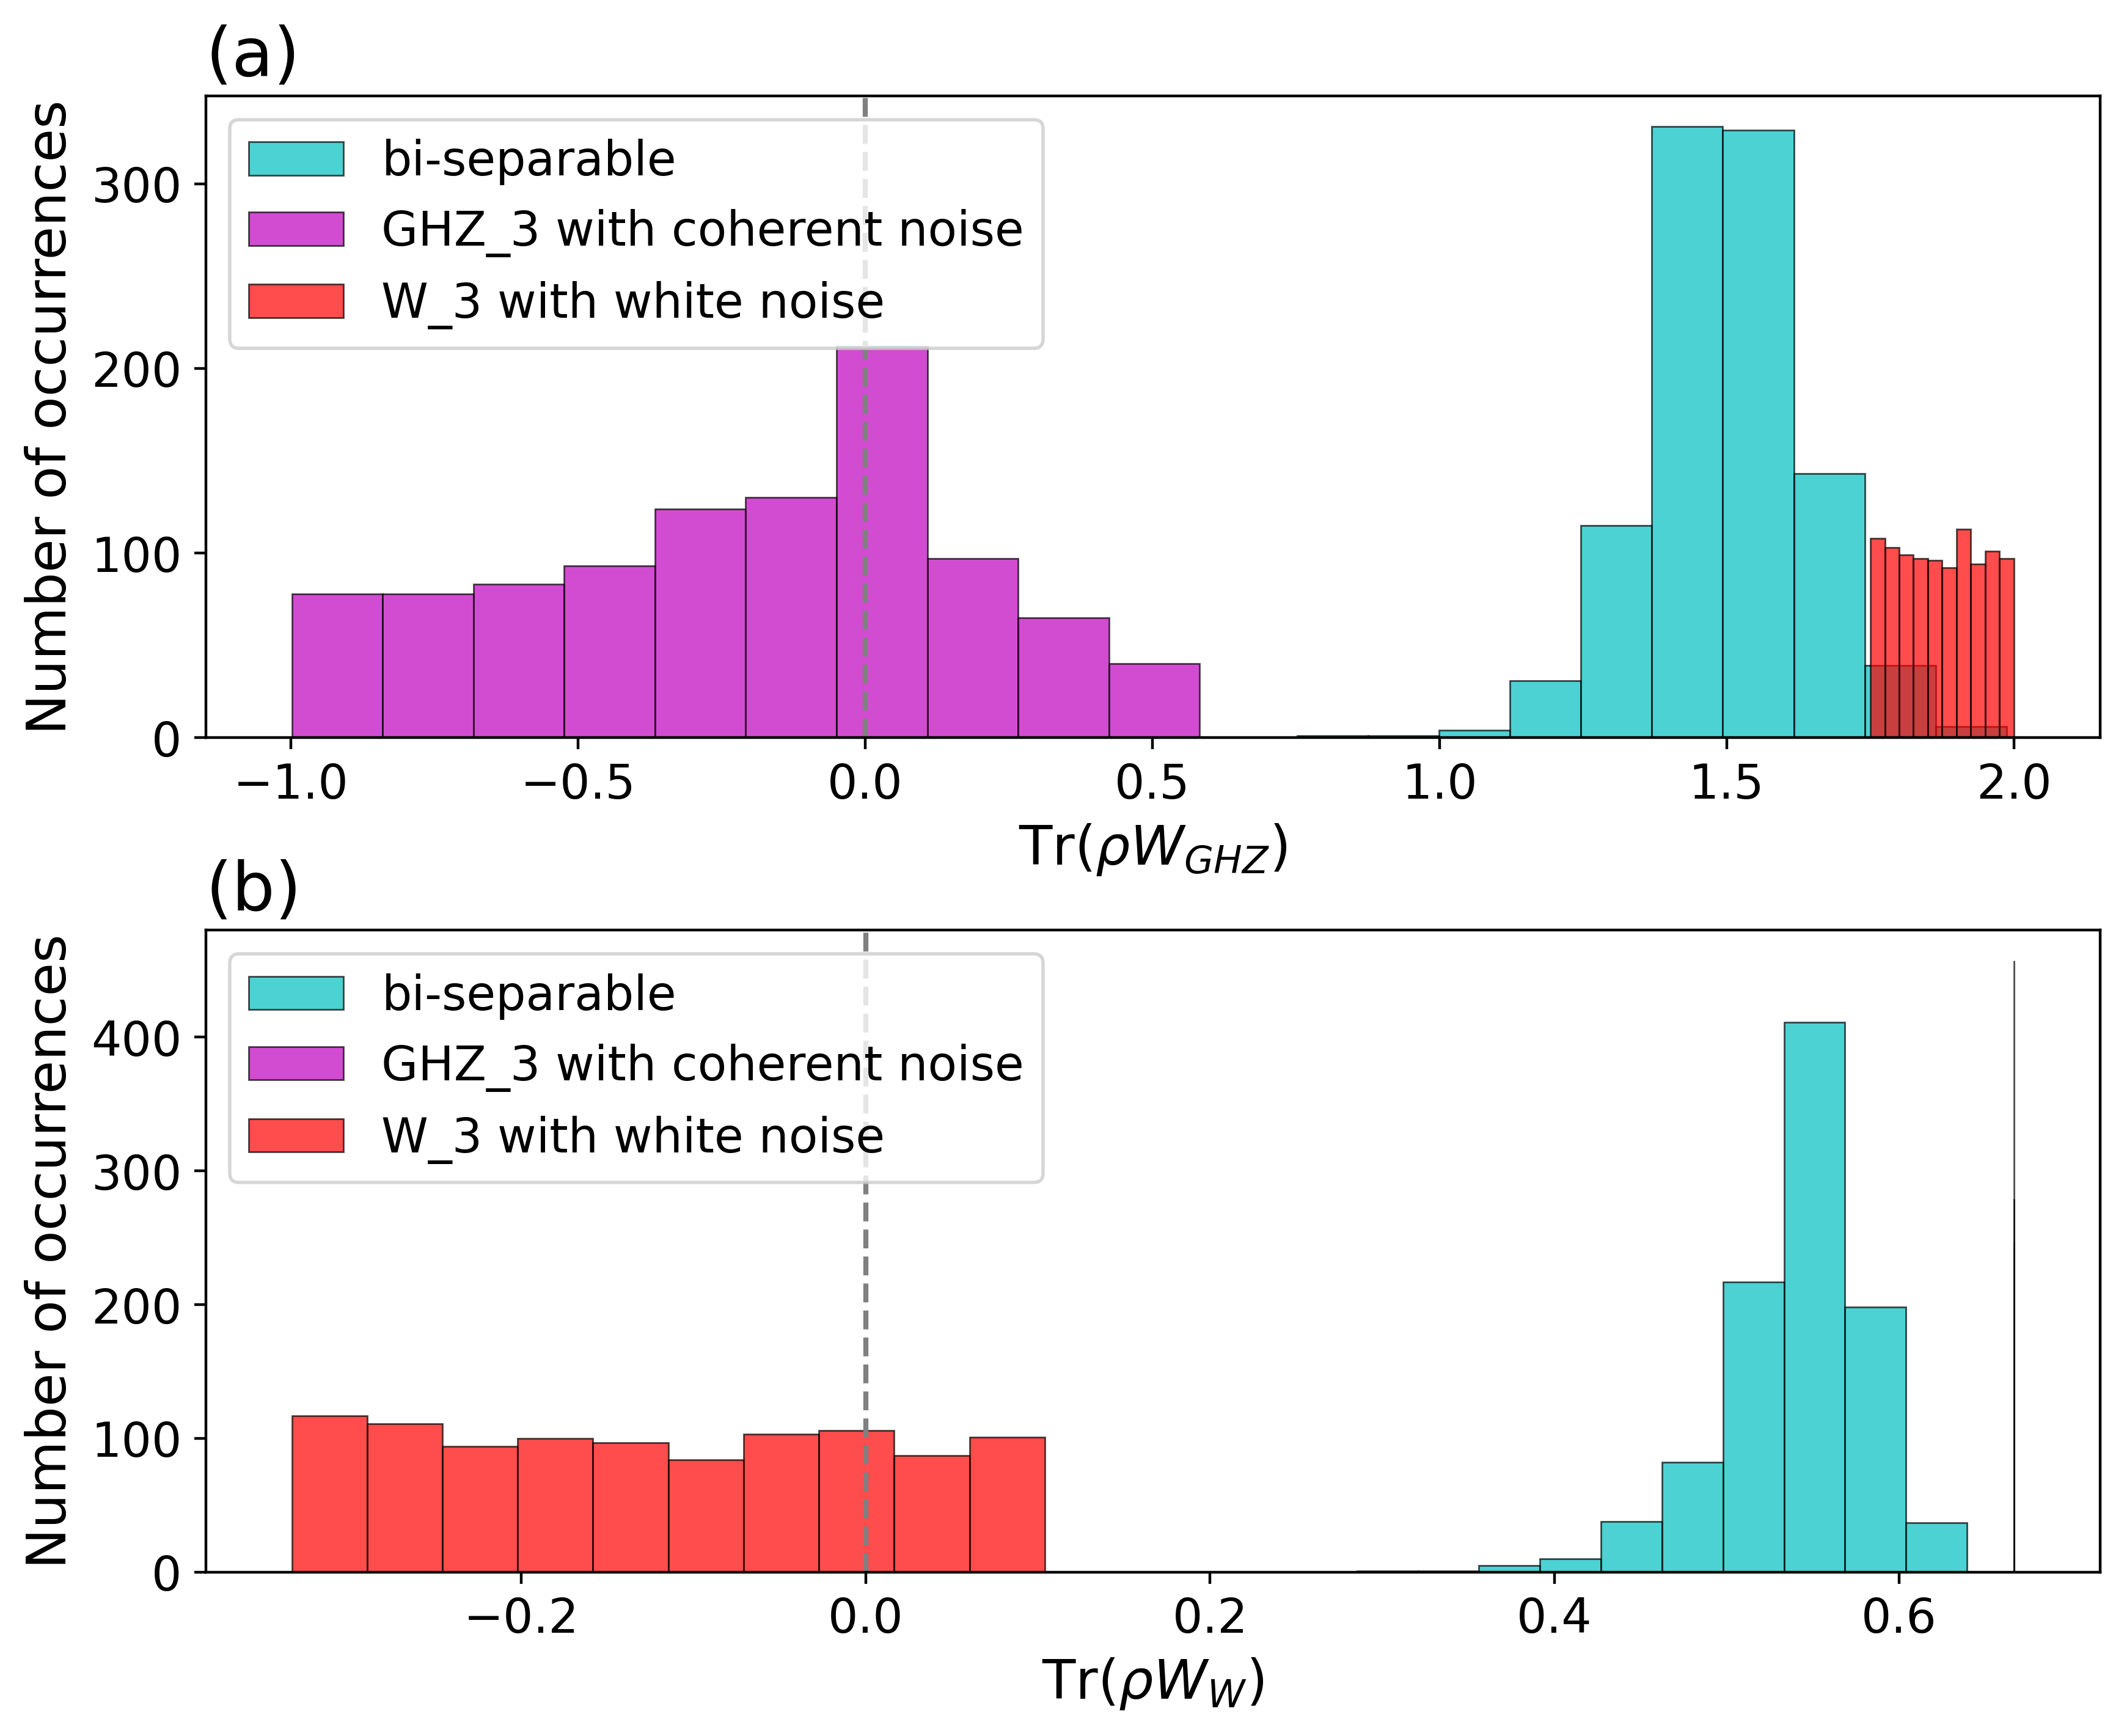
\includegraphics[width=.9\linewidth]{./Code/fidelity_witness_compare_2_long.png}
	\caption{Entanglement cannot be detected by fidelity witness (GHZ state with coherent noise, W state with large white noise)}
	% \caption{(a) compare different methods: Bell inequality, witness, ML ansatz; different white noise limit, unfaithful state; }
\end{figure}

To formally characterize the cases beyond fidelity witness, Weilenmann et. al \cite{weilenmannEntanglementDetectionMeasuring2020} coined the term \emph{unfaithful states} 
which systematically analyze 2-qudit entangled state mixed with white noise that cannot be detected by fidelity witness.
They found that for $d \ge 3$ that almost all states in the Hilbert space are unfaithful. 
% For $d > 5$, the authors find that all states they generated are entangled but at the same time unfaithful, regardless of what metric is used to sample them.
% faithful states are useful for quantum teleportation.
% This shows that fidelity-based entanglement witnesses detect entanglement that is useful for teleportation.
Subsequently, G\"{u}the et. al \cite{guhneGeometryFaithfulEntanglement2021} \cite{riccardiExploringRelationshipFaithfulness2021} give a formal definition: 
% the faithfulness of a twoqubit state, allowing for a physical interpretation of unfaithful two-qubit states as exactly those entangled states that are not useful for teleportation.
\begin{definition}[unfaithful state]\label{def:unfaithful_state}
	% informally, unfaithful state are entangled states but cannot be detected by fidelity witness.
	A 2-qudit state $\dm_{AB}$ is faithful if and only if there are local unitary transformations $\U_A$ and $\U_B$ such that
	\begin{equation}
		\expval{\U_A\otimes\U_B \dm_{AB} \U_A^\dagger \otimes\U_B^\dagger}{\phi^+}
		> \frac{1}{d}.
	\end{equation}
\end{definition}
Consequently, they found a necessary and sufficient condition for 2-qubit unfaithfulness, determined by the spectrum of
\begin{equation}
	\mathcal{X}_2( \dm_{AB})=\rho_{AB}-\frac{1}{2}(\dm_{A}\otimes \identity + \identity \otimes \dm_{B})+\frac{1}{2} \identity \otimes \identity
	\label{eq:unfaithful_2qubit},
\end{equation}
i.e.,
a 2-qubit state $\dm_{AB}$ is faithful if and only if the maximal eigenvalue of $\mathcal{X}_2( \dm_{AB})$ is larger than 1/2.
We can see in \cref{fig:unfaithfulness}, even for 2-qubit systems, nonnegligible portion of states are unfaithful but still entangled (NPT).
\begin{figure}[!ht]
	\centering
	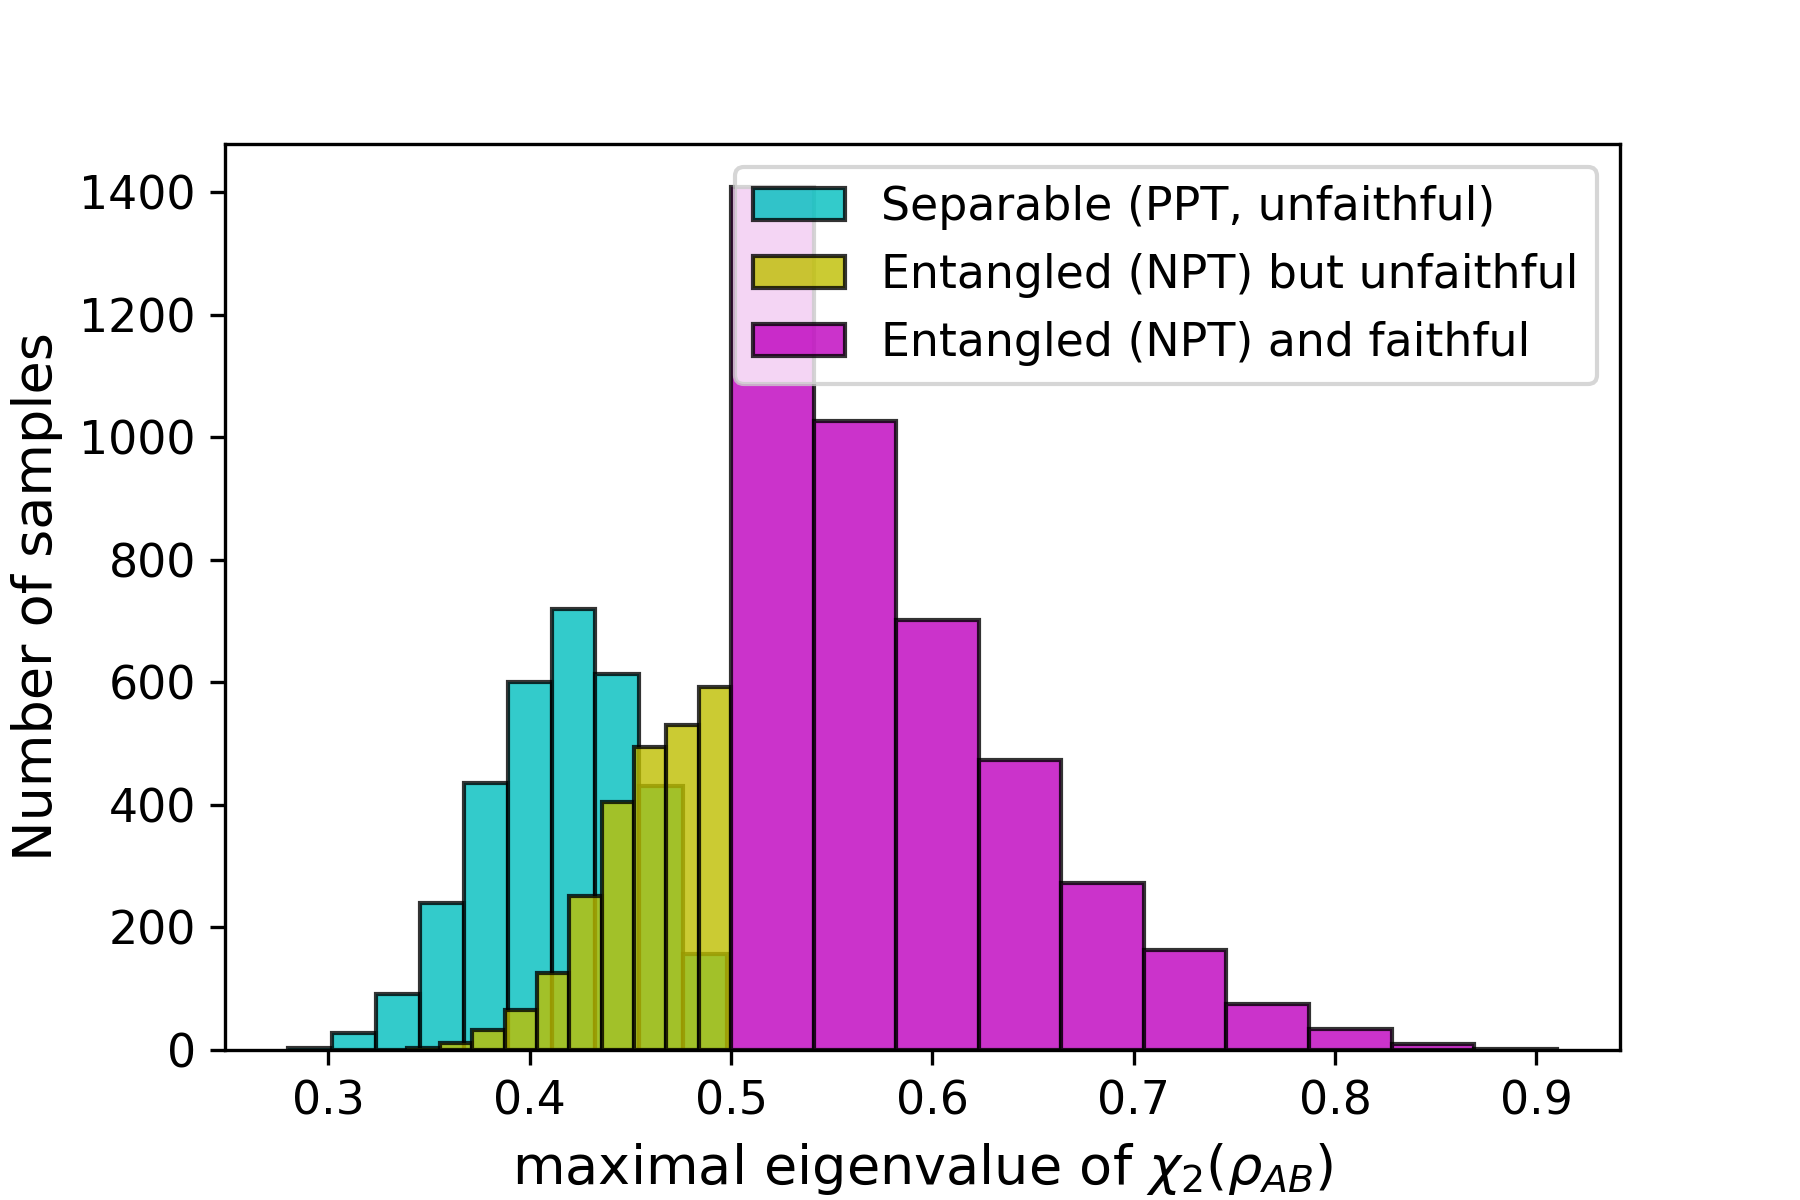
\includegraphics[width=.9\linewidth]{./Code/faithfulness_2_qubit.png}
	% \caption{PPT criterion (2-qubit random density matrix)}
	\caption{Unfaithfulness of 2-qubit states determined by the maximal eigenvalue of \cref{eq:unfaithful_2qubit}.}
	\label{fig:unfaithfulness}
\end{figure}

Although there are variants of witness \cite{zhouEntanglementDetectionCoherent2020}, such as nonlinear witness \cite{guhneNonlinearEntanglementWitnesses2006} and post-processing \cite{zhanDetectingEntanglementUnfaithful2021}, designed to remedy the shortcomings of conventional fidelity witness respectively, 
% \cite{huOptimizedDetectionHighDimensional2021}
it would be meaningful in practice to find a generic method to construct witnesses for \nameref{prm:entanglement_detection}.
% Moreover, they can only be applied to bipartite systems, which means they cannot be generalized to detect genuine entanglement in multipartite states.
Machine learning techniques satisfy the needs well because supervised learning can be regarded as a powerful nonlinear post-processing tool.


\subsection{Training a generic witness via SVM}
% \section{End-to-end entanglement detection protocol}\label{sec:protocol}
% \section{Classical-quantum hybrid, end-to-end detection protocol}
% \section{Classical, data-powered, and quantum algorithms}
% In this paper, we focus on the entanglement structure dectection for graph states.
The introductory task of classical machine learning (ML) is the binary classification,
such as cat/dog images classification. 
In (supervised) learning, the input to a ML algorithm is a (training) dataset $\qty{\vbx^{(i)},y^{(i)}}_{i=1}^m$ consists of $m$ data points, 
where each is a pair of feature vector $\vbx$ and its label $y$ (either 0 or 1).
For example, the feature $\vbx$ of an image is a flatten vector of all pixel values and the label $y=0(1)$ for \textsf{cat} (\textsf{dog}) respectively.
It is clear to see \nameref{prm:separability} or \nameref{prm:entanglement_detection} are exactly such binary classification problems where each quantum state has a binary label, such as  $\entangled$/\textsf{\nameref{def:bipartite_separable}}.
The features $\vbx$ of a quantum state $\dm$ can be the entries of its density matrix, or more realistically, the expectation values of certain observables.
% formally in \cref{sec:svm}
% The quantum extension of this problem (classficiation/pattern recognition) is to replace the data points with density matrices of quantum states . 
% Specifically, a quantum state classifier outputs a label associated with the state, such as, $\entangled$ or `bi-separable'.

With the surge of ML research, ML algorithms have been proposed for classification tasks related to entanglement.
Lu et. al \cite{luSeparabilityEntanglementClassifierMachine2018} 
trained a (universal) \nameref{prm:separability} classifier by classical neural network
where features are the entries of density matrices.
% where input dataset are (randomly sampled) density matrices  with labels?.
For the similar purpose, Ma and Yung \cite{maTransformingBellInequalities2018} generalized Bell inequalities to a Bell-like ansatz $\ew_{\ml}:=\vbw_{\ml}\cdot\vb{\pob}_{\bellineq}$ where the optimal weights $\vbw_{\ml}$ are obtained via a neural network.
% an ansatz for \nameref{def:entanglement_witness} 
% Different Bell inequalities can be regarded as entanglement witness for different types of entanglement in a multi-party entangled state.
% (graph state entanglement)
And they found the tomographic ansatz
\begin{equation}
	\ew_{\ml} := 
	\vbw_{\ml} \cdot \vb{\pob}_{\sigma} \, , \; \forall \sigma \in  \qty{I,X,Y,Z}^n
	% \sum_{k_1,k_2,\dots,k_n}  w_{k_1,k_2,\dots,k_n} \bigotimes_i^n \hat{\sigma}^{(k_i)}
	% ,\quad \hat{\sigma} \in \qty{\sx,\sy,\sz,\identity_{2\times 2}}
	% \sum_{\vb{p}\in \qty{I,X,Y,Z}^n} w_{\vb{p}}  \bigotimes_i^n \vb{p}_i
	% \hat{\sigma}^{(\vb{p}_i)}
	\label{eq:tomographic_ansatz}
\end{equation}
% c.f. \nameref{prm:full_tomography} 
has better performance, 
also required \cite{luTomographyNecessaryUniversal2016} for a universal \nameref{prm:separability} classifier.
It is worth noting that training a universal classifier for high-dimensional systems is hard if the gap between two state sets is small (weak promise).

\begin{figure}[!ht]
	\centering
		\centering
		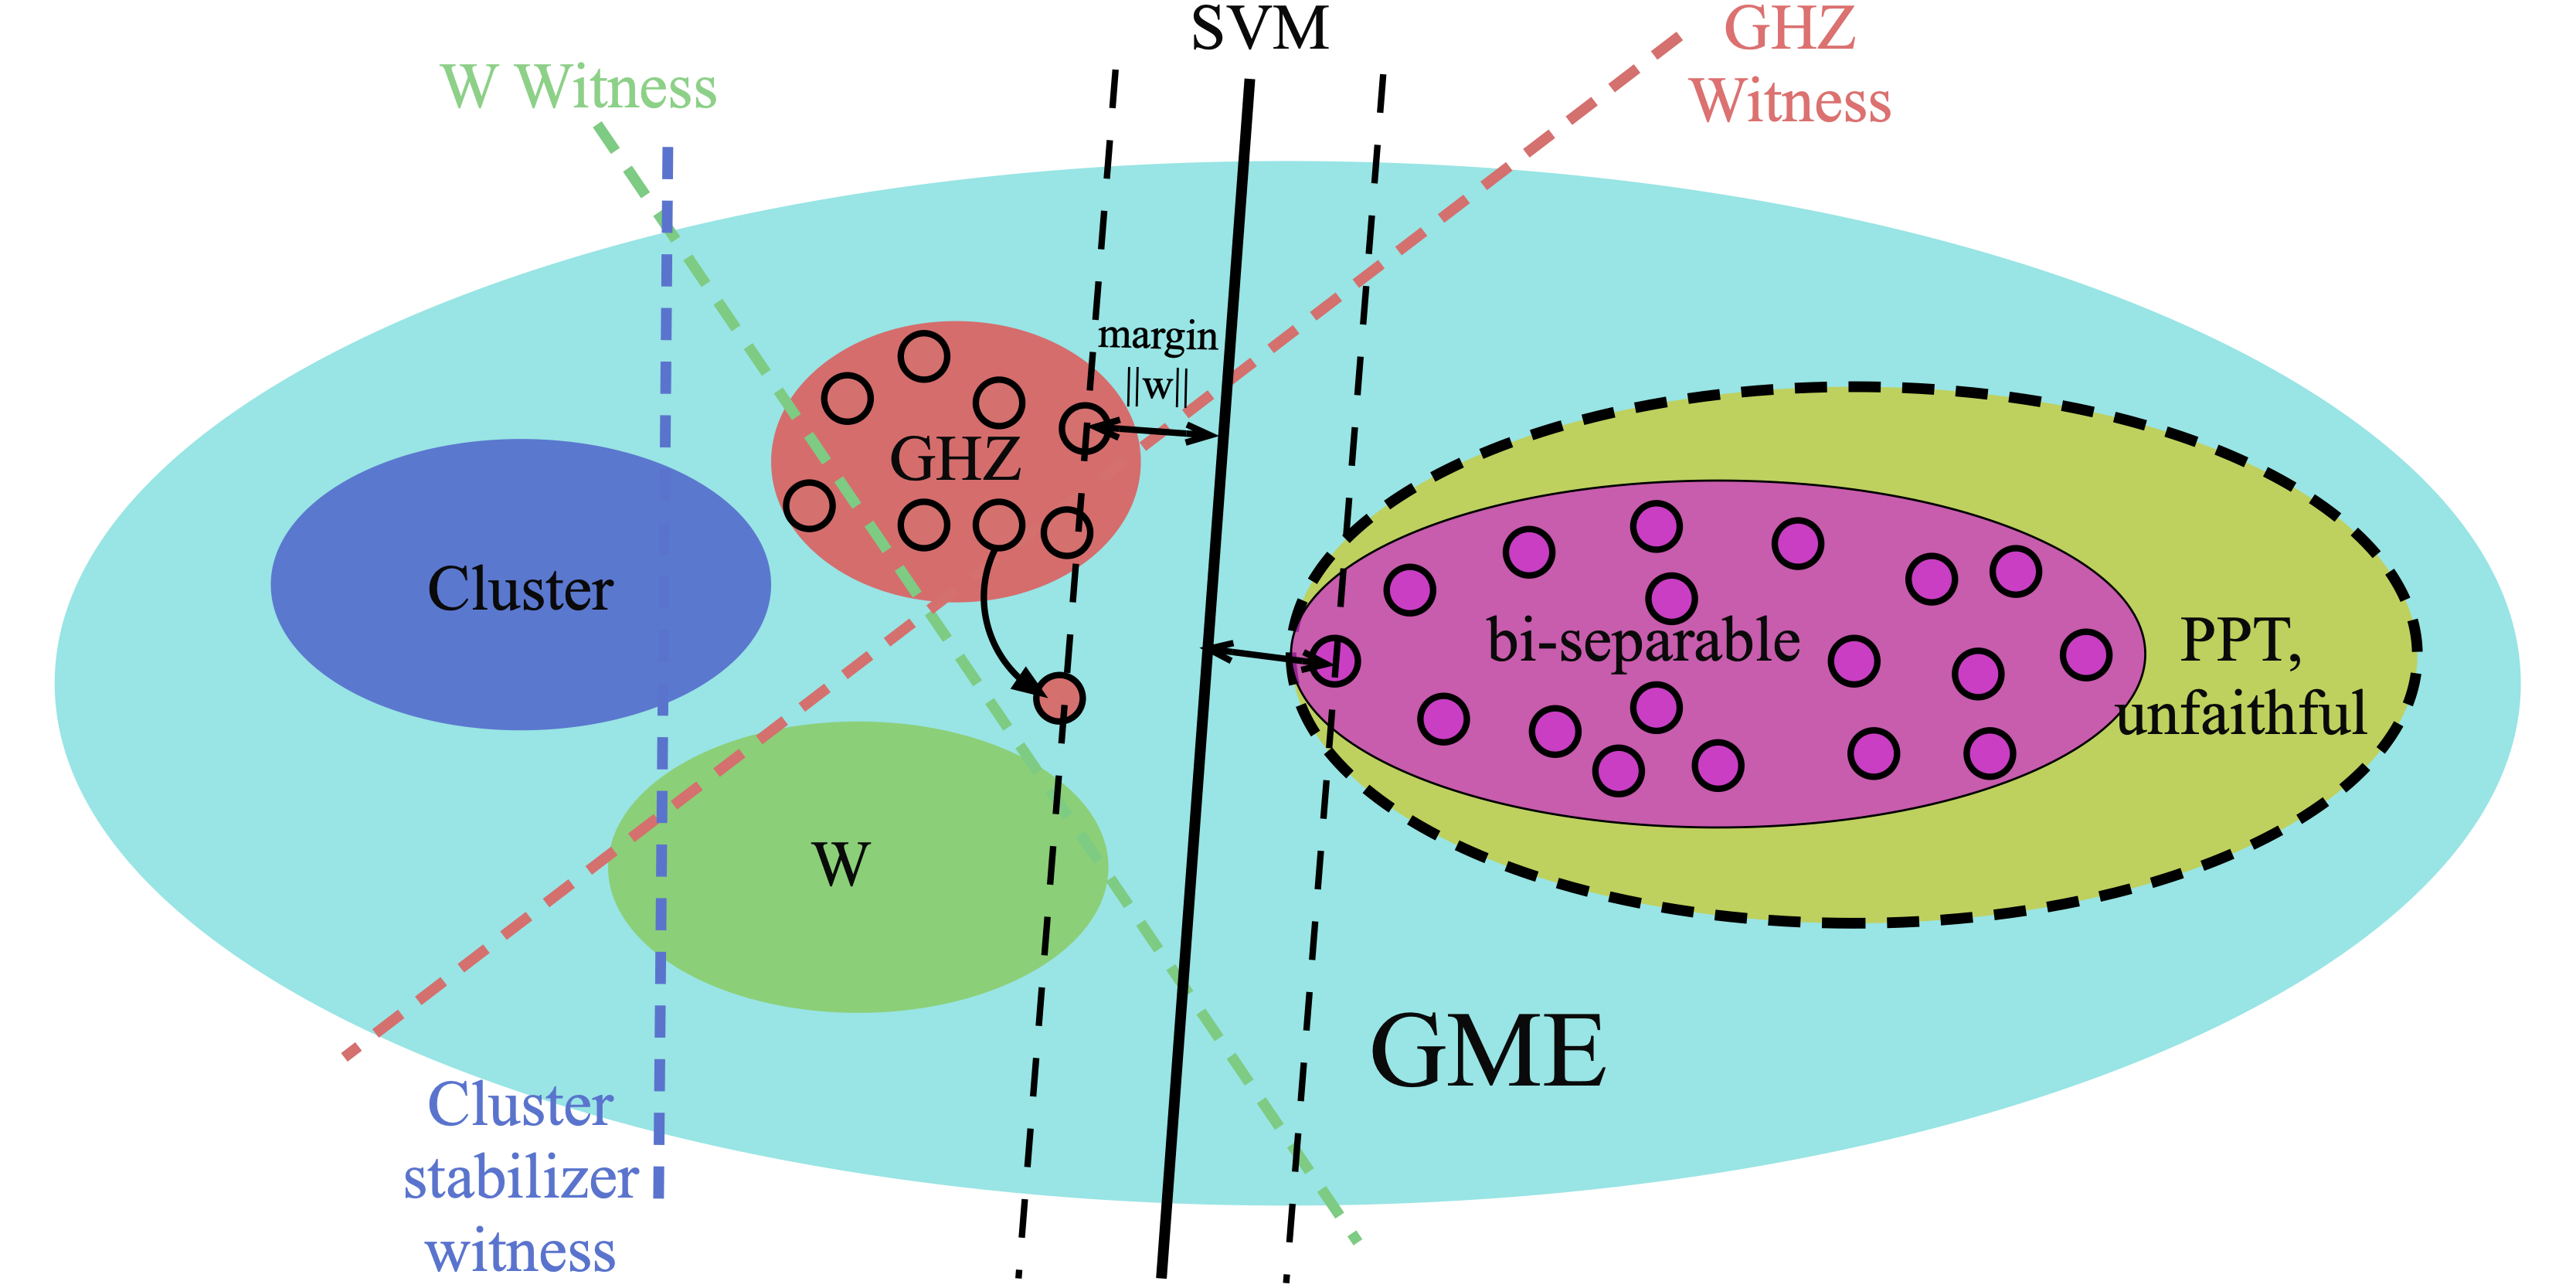
\includegraphics[width=.8\linewidth]{schematic_entangle.png}
	% 	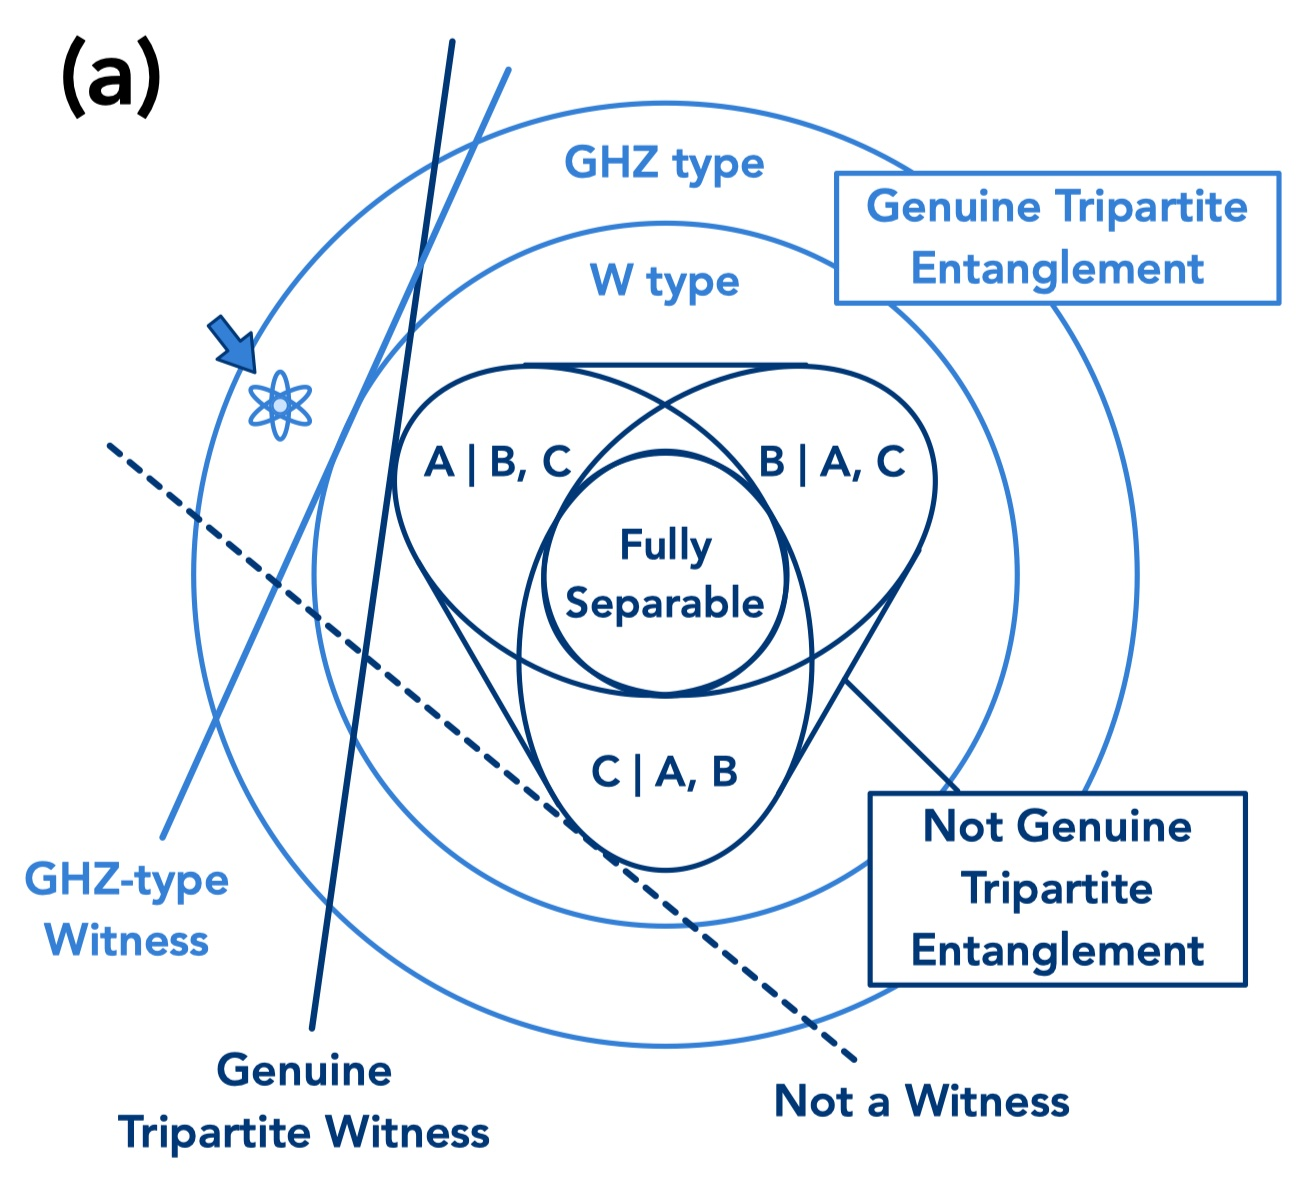
\includegraphics[width=.9\linewidth]{gme.jpg}
	% . 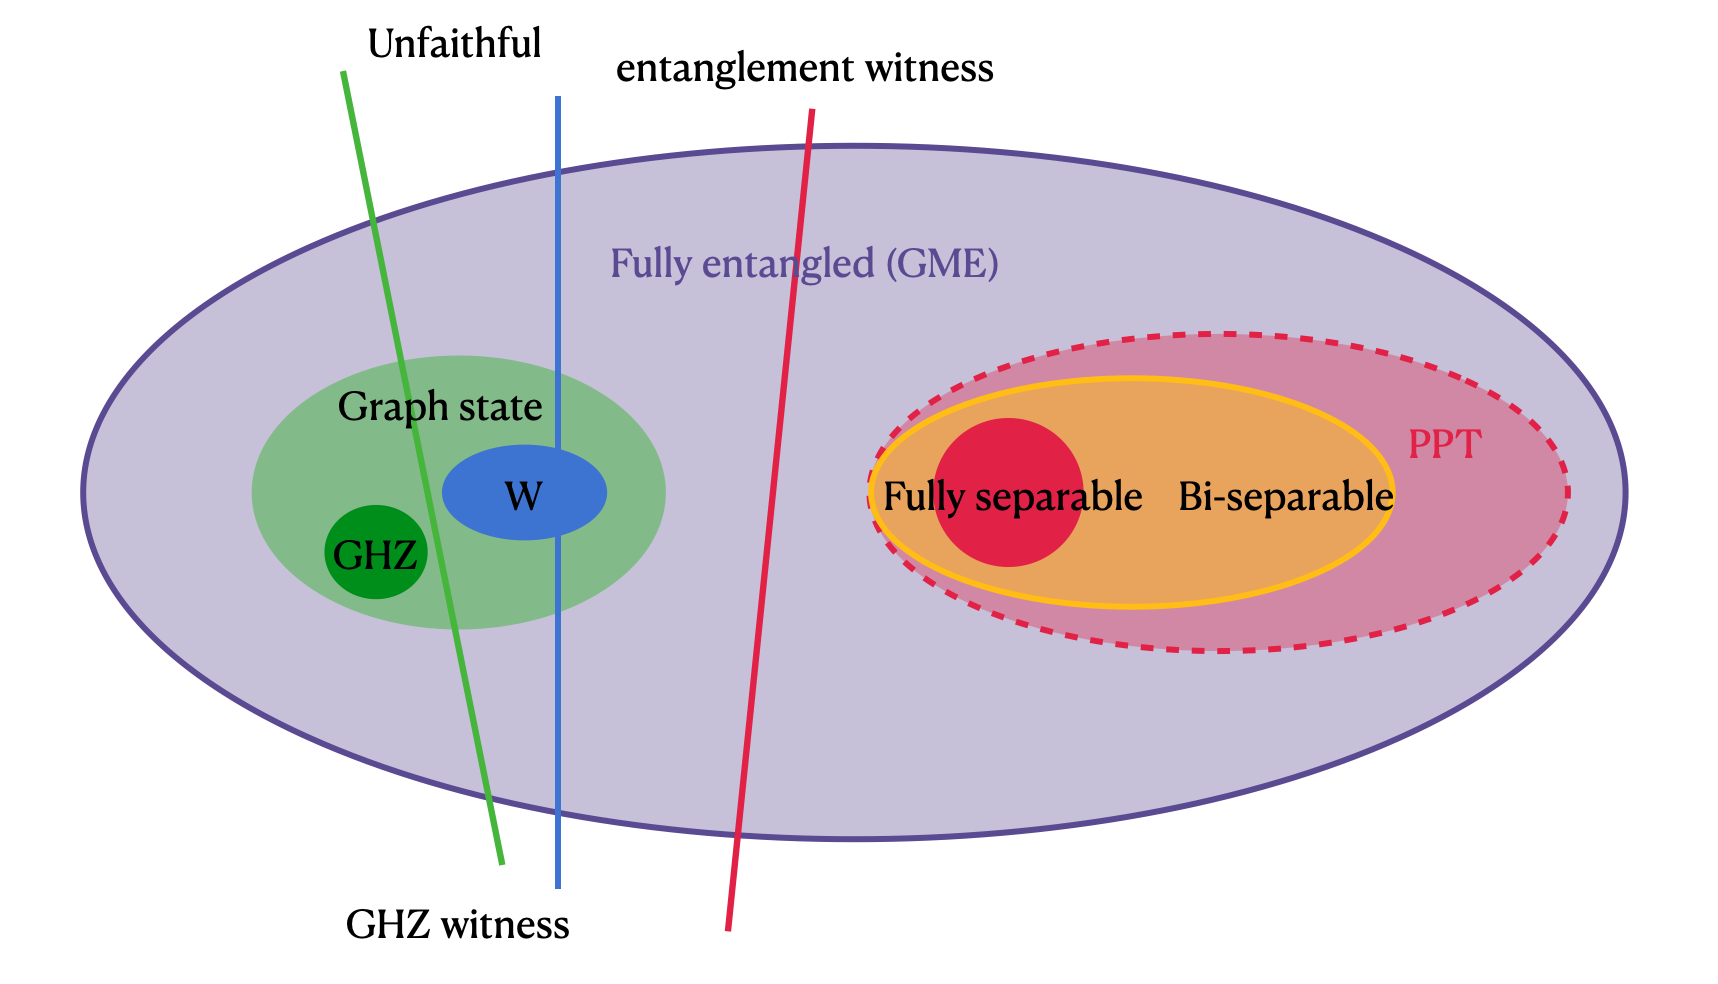
\includegraphics[width=.7\linewidth]{witness.png}
	% 	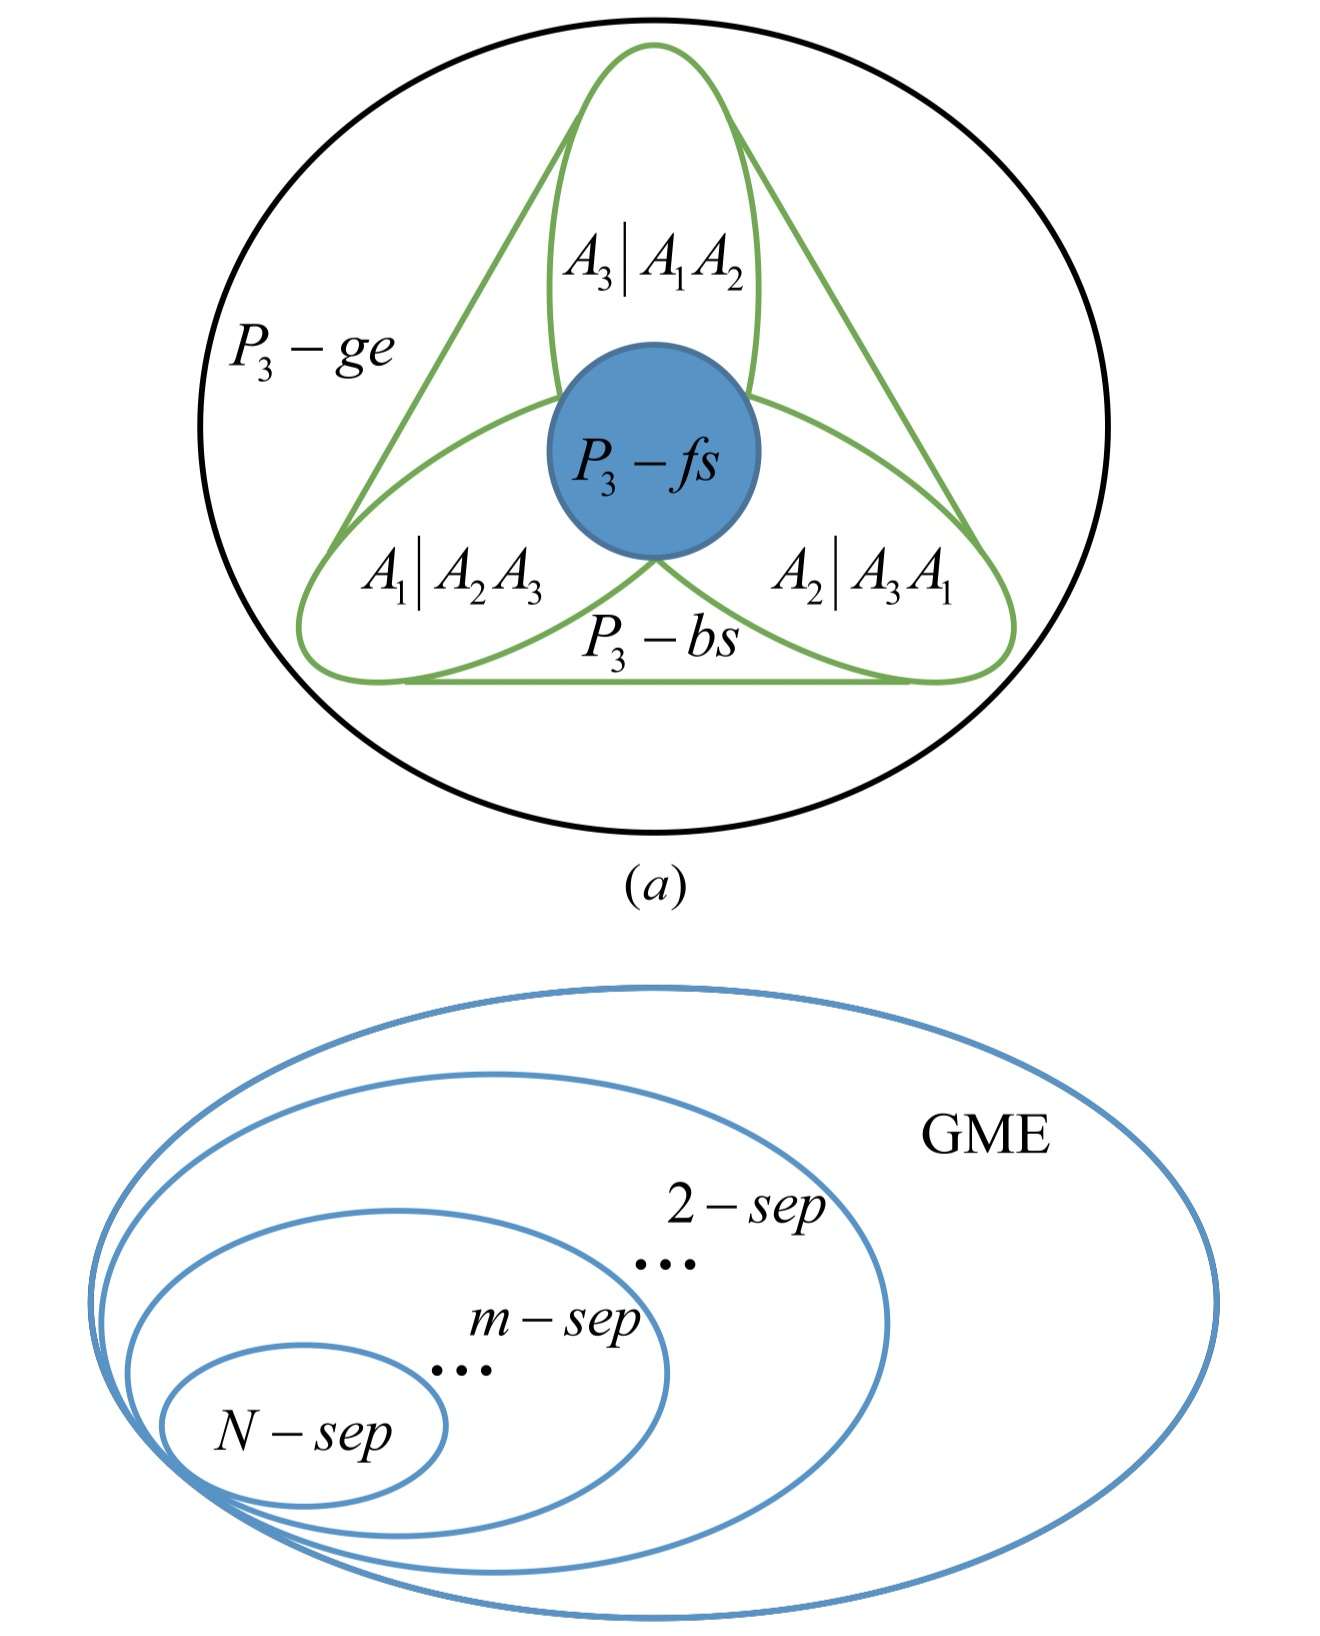
\includegraphics[width=.8\linewidth]{sep.jpg}
	% 	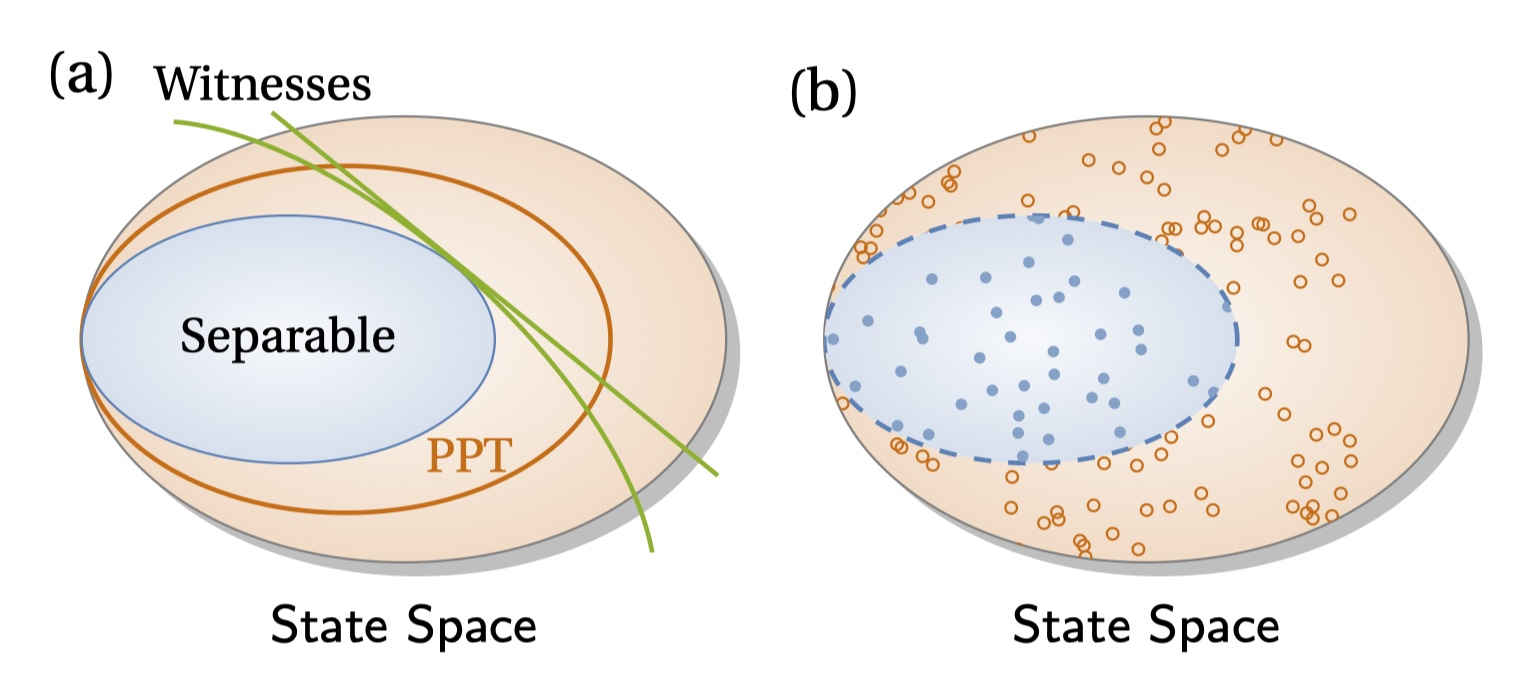
\includegraphics[width=.9\linewidth]{ppt.jpg}
	\caption{Schematic diagram for entanglement detection methods: entanglement witnesses for different states are depicted by colored dash lines (hyperplane). \nameref{def:svm} with the linear kernel (hyperplane). \nameref{thm:ppt} (non-linear, one-side) ... }
	\label{fig:entangle}
\end{figure}

% \subsection{Training a generic witness via SVM}
In our paper, we focus on the problem \nameref{prm:entanglement_detection} with training data.
In other words, we derive the entanglement witness for certain target states with desired entannglement structure by fitting a synthetic dataset.
\begin{problem}[Learn an entanglement witness]\label{prm:learn_witness}
	learn a witness for \nameref{prm:entanglement_detection} of $\dm$ from data
	\begin{itemize}
		\item \textbf{Input}:  synthetic data consist of density matrices $\dm$ with corresponding labels $y$
		\item \textbf{Output}: a (minimal) classifier $\vbw_{\ml}$ with high accuracy
	\end{itemize}
\end{problem}

% \begin{problem}[detect graph state entanglement structure?]
% 	problem with/without training data
% 	\begin{itemize}
% 		\item \textbf{Input}: a graph $\graph$ encoding in a graph state $\ket{\graph}$;
% 		adjacency matrix $A$?
% 		\item \textbf{Output}: entanglement structure: \textsf{\nameref{def:gme}}??
% 	\end{itemize}
% % with training data: 
% \end{problem}
% \begin{itemize}
% 	\item \textbf{features}: classical shadow?
% 	\item label: 
% \end{itemize}

% \subsubsection{Variational quantum kernel estimation (hybrid)}
% \subsection{Variational (hybrid) quantum algorithms}
% \subsubsection{Related works}
% \begin{itemize}
% \item 

% (feature: synthetic density matrix with noise flatten as a real vector $\vbx\in\realnumber^{d_A^2d_B^2-1}$). 
% (label: separable or entangled by \nameref{thm:ppt}, CHA), and then train the classifier to predict the class labels of new states that it has not encountered before.
% Previous methods \textbf{only detect a limited part of the state space}, e.g. different entangled states often require different \nameref{def:entanglement_witness}. 
% \item 

% it is difficult to generate general GME states or label general states.
% Tomography is necessary for universal entanglement detection with single-copy observables (non-adaptive schemes) \cite{luTomographyNecessaryUniversal2016}
% However, the challenge is to find a reliable way for labelling the quantum states in the training set.
% Overall, for scaling up this method for detecting higher-dimensional quantum entanglement, the major challenge is related to a lack of reliable method for labeling the entanglement.
% We have constructed such a universal state classifier for a pair of qubits; we find that the performance depends heavily on the testing sets; the major source of error comes from the data near the boundary between entangled and separable states.
% Tomographic predictors make use of all information of a given quantum state and is used to benchmark the performance of Belllike predictors, which employs a subset of non-orthogonal measurements setting.
% \begin{remark}
% \cite{luSeparabilityEntanglementClassifierMachine2018} reported that they independently combined machine learning and semidefinite programming to train their predictors as quantum state classifiers. Using all information without any prior knowledge, the error of their predictor is always around 10\% on general 2-qubit system. However, our tomographic predictor performs below 2\% on the same ensembles with 3000 hidden neurons.
% \end{remark}

\nameref{prm:learn_witness} problem has also been studied by classical ML \cite{zhuMachineLearningDerivedEntanglement2021}  \cite{vintskevichClassificationFourqubitEntangled2022}, 
but by a different technique called Support Vector Machine (\nameref{def:svm})  \cite{cortesSupportvectorNetworks1995}.
% (Stokes parameters) \cref{eq:stokes_tomography}.
The features $\vbx:=\Tr(\dm\pob_{\sigma})$ of a state is a vector of expectations of Pauli observables.
An SVM constructs a hyperplane $\expval{\ew_{\svm}}=\vbw_{\svm} \cdot \vbx$ that clearly delineates two kinds of states, see \cref{fig:entangle}.
% (bipartite and \textbf{tripartite qubit and qudit}); 
% SVM shares the very similar geometric interpretation with entanglement witness, see \cref{fig:entangle}.  
% (cf. \cref{eq:entanglement_witness}, \cref{eq:svm_opt} and \cref{fig:entangle}).
Both SVM witness and conventional fidelity witness is a weighted sum of observables (features) which represents a hyperplane in the state (feature) space.
The SVM witness is more flexible because coefficients are optimized (automatically derived) from training.
% for a generic state with desired entanglement structures.
This method only requires local (Pauli) measurements even when the target state is a non-stabilizer state, such as W state (normally need nonlocal measurements).

\begin{algorithm}[H]
    \DontPrintSemicolon
    \SetKwInOut{Input}{input}
    \SetKwInOut{Output}{output}
    \Input{states with labels: $\qty{(\dm^{(i)},y^{(i)})}^m_{i=1}$}
    \Output{a classifier $\vbw_{\ml}$, $\bmsigma_{\ml}$}
    \BlankLine
	% \tcp*{---------------------------------------------- training phase ------------------------------------------------}
	% \tcc{training phase}
	Evaluate Pauli observables $\vbx^{(i)}_{\dm,\bmsigma}:=\Tr(\dm^{(i)}\pob_{\bmsigma})$,  $\forall i$ \\
    \For{ $j = 1,2, \ldots, 4^n$} {
		\While{  accuracy not high enough} {
			randomly select $j$ features $\tilde{\vbx}_i$ from $\vbx_i$, $\forall i$ \\
			% kernel estimation \tcp*{classical kernel}
			accuracy, classifier = SVM($\qty{(\tilde{\vbx}_i,y_i)}^m_i$)
			% \tcp*{train SVM}
			% \tcc{comment in a new line}
		}
    {\Return classifier $\vbw_{\ml}$} 
	% \tcp*{parameters of the separating hyperplane in the feature space}
    }
	% \tcp{call Algorithm. \ref{alg:classical_shadow}}
	% \tcp*{============================================= prediction =============================================== //}
	% Test the classifier on test dataset
    % \Return $ \vb{w}\cdot \vec{\sigma}<0 $: \textsf{separable} 
	% \tcc{predict}
	% \tcc{testing phase}
	% \tcp*{============================================= testing phase =============================================== //}
    \caption{train a witness via kernel \nameref{def:svm} }
    \label{alg:classical_learning}
\end{algorithm}

A key drawback (constrain) of conventional witnesses is its linearity.
Despite the non-linear witness \cite{guhneNonlinearEntanglementWitnesses2006} proposed, its implementation in experiments is more challenging than linear one.
The good news is,
within the framework of SVM, non-linearity can be easily achieved by the \nameref{def:kernel} method.
We focus on kernel methods rather than neural networks (also non-linear), 
not only because of its clear geometric interpretation, but also its equivalence to neural network in terms of neural tangent kernel \cite{jacotNeuralTangentKernel2020}.
% as they not only provide provable guarantees, but are also very flexible in the functions they can learn. 
% For example, recent advancements in theoretical machine learning show that training neural networks with large hidden layers is equivalent to the neural tangent kernel \cite{jacotNeuralTangentKernel2020}.
The advantages of SVM: (1) the training of an SVM is convex; if a solution exists for the given target state and ansatz, the optimal SVM will be found.
(2) this SVM formalism allows for the programmatic removal of features, i.e., reducing the number of experimental measurements and copies (samples). 
% in exchange for a lower tolerance to white noise, in a manner similar to [??].
% \item 
% SVM, (universal), 4 qubit.
% \item 
% \end{itemize}

% \subsubsection{Our witness ansatz and optimization}

\begin{table}[!ht]
	\centering
	\begin{tabular}{c|c|c|c}
		& \# observables & weights & promise \\
		\hline
		% entanglement witness & & & known \\  
		fidelity  witness & few local & fixed & strongest  \\  
		% convex?\cite{chakrabartiQuantumAlgorithmsLower2020} 
		Bell (CHSH) inequality & constant & fixed & weak \\  
		% entangle spectrum \cite{horodeckiDirectDetectionQuantum2002} & & & unknown \\  
		tomographic classifier & $4^n-1$ & trained & weakest \\  
		SVM (kernel) witness &  $\ll 4^n-1$ & trained & strong \\  
		\hline
	\end{tabular}
	\caption{Comparison of CHSH inequality, fidelity witness, and ML witness ansatz.}
\end{table}

However, these previous ML witnesses only consider the robustness to white noise and cannot be directly applied to experiments.
%  because they didn't address the problem of estimating classical features. 
In numerical simulation, we can efficiently evaluate classical features by direct calculation, 
but, in actual experiments, entries of a density matrix are not explicitly known.
Instead, we need to estimate the observables by many measurements, which we will discuss in next section.


% \subsubsection{Variational entanglement witness (ansatz)}

\subsection{Sample-efficient expectation estimation methods}\label{sec:estimation}
% \subsection{Estimate classical features of quantum states}
% To apply classical machine learning classifier (SVM) in actual experiments, we need classical features of quantum states.
% Nevertheless, we cannot directly evaluate expectation values as in numerical simulation because we do not know density matrices of incoming states.
% \textbf{features}: classical shadow? raw data? quantum data, label: entangled?
% \subsection{Tomography and trace estimation}
% \label{sec:shadow_tomography}
The brute force approach to fully characterize a state in an experiment is quantum state tomography \cite{altepeterPhotonicStateTomography2005}
\footnote{Informally, quantum state tomography refers to the task of estimating complete description (density matrix) of an unknown $D$-dimensional state $\dm$ within error tolerence $\epsilon$, 
given the ability to prepare and measure copies of $\dm$.}.
With a recovered densitry matrix, we can directly calculate classcial features or separability measures,
but full tomography is experimentally and computationally demanding.
% \begin{problem}[quantum state tomography]\label{prm:full_tomography}
% 	Informally, quantum state tomography refers to the task of estimating complete description (density matrix) of an unknown $D$-dimensional state $\dm$ within error tolerence $\epsilon$, 
% 	given the ability to prepare and measure copies of $\dm$.
% 	% measure $m$ copies $\dm^{\otimes m}$.
% 	% \begin{equation}\label{eq:stokes_tomography}
% 	% 	\dm = \frac{1}{2^n} \sum_{i_1,i_2,\dots,i_n=0}^3
% 	% 	S_{i_1,i_2,\dots,i_n} 
% 	% 	\hat{\sigma}_{i_1} \otimes \hat{\sigma}_{i_2} \otimes \dots \otimes \hat{\sigma}_{i_n} 
% 	% 	\begin{itemize}
% 	% 		\item \textbf{Input}: Given a \textbf{unknown} $N$-dimensional mixed state $\dm$
% 	% 		\item \textbf{Output}:
% 	% 	\end{itemize}
% 	% \end{equation}
% \end{problem}
% The canonical representation (decomposition) of a $n$-qubit density matrix
% is $\dm=2^{-n} \sum_{\bmsigma \in \qty{I,X,Y,Z}^n} t_{\bmsigma}  \ob_{\bmsigma} $  
% % is $\dm=2^{-n} \sum_{\vb{p}\in \qty{I,X,Y,Z}^n} t_{\vb{p}} \bigotimes_i^n \vb{p}$  
% \cite{altepeterPhotonicStateTomography2005}.
	% Stokes decomposition
% Since there are $D^2$ entries in a density matrix, navie full tomography based on independent measurements need at least $D^2$ copies.
Even if adaptive or collective measurements (and post-processing) allowed 
\footnote{Intermediate between independent measurements and unrestricted (also called “collective” or “entangled”) measurements are adaptive measurements in which the copies of $\dm$ are measured individually, but the choice of measurement basis can change in response to earlier measurements.},
rigorous analysis \cite{haahSampleoptimalTomographyQuantum2017} \cite{odonnellEfficientQuantumTomography2016} proved that 
$\Omega(D^2/\epsilon^2)$ measurements (copies?)  are required for recovering a $D\times D$ density matrix
% $\Omega(Dr/\epsilon^2)/\log(D/r\epsilon)$ copies/measurements are required for a $D$-dimensional ($D=2^n$ for $n$-qubit systems), rank-$r$ density matrix 
with error tolerence $\epsilon$ measured in trace \nameref{def:distance}.


% \begin{problem}[Fidelity estimate]
% 	defined as follows
% 	\begin{itemize}
% 		\item \textbf{Input}: Given two density matrices $\dm$ and $\dm'$, 
% 		\item \textbf{Output}: \nameref{def:fidelity} with error $\epsilon$
% 	\end{itemize}
% \end{problem}
Now that full tomography is not practical for large systems, a natural question is whether it is possible to extract a bunch of information about a state without fully recovering it.
The answer is yes.
Many interesting properties of a quantum system are often linear functions of the underlying density matrix $\dm$, such as classical features $x_{\dm,\sigma}=\Tr(\dm\pob_{\sigma}) $ for entanglement witness
\footnote{nonlinear functions: \nameref{def:entropy};
multivariate functions:  $\Tr(\dm_1 \cdots \dm_m)$, \nameref{def:quantum_kernel} $\Tr(\dm\dm')$,  quadratic $\Tr(\ob \dm_i \otimes \dm_j)$, \nameref{def:fidelity} $F(\dm,\dm')$.}.
% \begin{problem}[trace estimation]\label{prm:trace_estimation}
% 	related problems defined as follows
% 	\begin{itemize}
% 		\item \textbf{Input}: Given an observable (Hermitian) $\ob$ and (copies of) a mixed state $\dm$ or several states ($\dm',\dots,\dm_m$), 
% 		\item \textbf{Output}: 
% 		with error $\epsilon$ measured by trace \nameref{def:distance} (\nameref{def:fidelity}...), to estimate
% 		linear functions (mostly): the expectation value $\expval{\ob}=\Tr(\ob \dm) $, entanglement witness, tomography; 
% 		nonlinear functions: \nameref{def:entropy};
% 		multivariate functions:  $\Tr(\dm_1 \cdots \dm_m)$, \nameref{def:quantum_kernel} $\Tr(\dm\dm')$,  quadratic $\Tr(\ob \dm_i \otimes \dm_j)$, \nameref{def:fidelity} $F(\dm,\dm')$, \nameref{def:distance}??;
% 	\end{itemize}
% \end{problem}
% Nevertheless, we usually only need specific properties of a target state rather than full classical descriptions about the state.
This enables the possibility to \emph{shadow tomography} \cite{aaronsonShadowTomographyQuantum2018}.
\begin{problem}[shadow tomography]\label{prm:shadow_tomography}
	Aaronson's formulation	
	($\probability[E_i \text{ accept } \dm]=?\Tr(E_i \dm)$)
	\begin{itemize}
		\item \textbf{Input}: copies of an unknown $D$-dimensional state $\rho$ and $M$ known 2-outcome measurements $\qty{E_1,\dots,E_M}$
		\item \textbf{Output}: estimate $\probability[E_i \text{ accept } \dm]$ to within additive error $\epsilon$, $\forall i\in [M]$, with $\ge 2/3$ success probability.	
	\end{itemize}
\end{problem}
\begin{theorem}[\cite{aaronsonShadowTomographyQuantum2018}]\label{thm:shadow_tomography}
	It is possible to do \nameref{prm:shadow_tomography} using $\tilde{\bigO}(\log^4 M\cdot \log D\cdot\epsilon^{-4})$ copies
	\footnote{full tomography: additive error $\epsilon\ll 1/D$.}.
	sample complexity lower bound $\Omega(\log (M) \cdot \epsilon^{-2})$, 
\end{theorem}
% \begin{theorem}[lower bound of \nameref{prm:full_tomography}?\cite{haahSampleoptimalTomographyQuantum2017}]
	% Though formally “efficient” in the sense that $N$ scales polynomially with $m$ for any fixed approximation error $\epsilon$, 
% \end{theorem}
Though it is proved that \nameref{prm:shadow_tomography} can be implemented in a samples-efficient (copies) manner,
Aaronson's shadow tomography procedure is very demanding in terms of quantum hardware.
So, Huang et. al \cite{huangPredictingManyProperties2020} introduce classical shadow (CS) method that is more friendly to experiments.
In our pipeline, we focus on the classical shadow method and its variants.
% \begin{remark}[compare shadow tomography with classical shadow \cite{huangPredictingManyProperties2020}]
% 	While very efficient in terms of samples, Aaronson's procedure is very demanding in terms of quantum hardware - a concrete implementation of the proposed protocol requires \textbf{exponentially long quantum circuits} that act collectively on all the copies of the unknown state stored in a quantum memory.
% 	% [compare shadow tomography and classical shadow ??]
% \end{remark}
% \subsubsection{Estimate expectations via classical shadow}\label{sec:classical_shadow}

A classical shadow is a succinct classical description of a quantum state, which can be extracted by performing reasonably simple single-copy measurements on a reasonably small number of copies of the state.
The classical shadow attempts to approximate this expectation value by an empirical average over $R$ independent samples, much like Monte Carlo sampling approximates an integral.
	\begin{equation}
		o_i = \Tr(O_i \dm_{\cs})
		\text{ obeys }
		\expectation[o] =\Tr(O_i \dm)
	\end{equation}
% \nameref{def:classical_shadow} \cite{huangPredictingManyProperties2020}: estimate entanglment witness (fixed but unknown target state, e.g., tripartite GHZ)
% \textbf{Classical shadows (Clifford measurements) of logarithmic size allow for checking a large number of potential entanglement witnesses simultaneously}.
% Directly measuring $M$ different entanglement witnesses requires a number of quantum measurements that scales (at least) linearly in $M$. In contrast, classical shadows get by with $\log(M)$-many measurements only.
classical shadows are based on random Clifford measurements and do not depend on the structure of the concrete witness in question. In contrast, direct estimation crucially depends on the concrete witness in question and may be considerably more difficult to implement.
% The transformation $U$ is randomly selected from an ensemble of unitaries, and different ensembles lead to different versions of the procedure that have characteristic strengths and weaknesses.

% more details in \cref{sec:classical_shadow}

% \begin{definition}[classical shadow]\label{def:classical_shadow}
% 	The classical shadow of a state $\dm$ is a ...
% 	such that we can predict the linear function with it
% 	\begin{equation}
% 		o_i = \Tr(O_i \dm_{\cs})
% 		\text{ obeys }
% 		\expectation[o] =\Tr(O_i \dm)
% 	\end{equation}
% \end{definition}

% \begin{algorithm}[H]
%     \DontPrintSemicolon
%     \SetKwInOut{Input}{input}
%     \SetKwInOut{Output}{output}
%     \Input{(copies of) density matrix $\dm$, an entanglement witness (observable) $\ew$}
%     \Output{$\Tr(P_x \dm ), \forall x \in \qty{ I, X, Y, Z }^n$}
%     \BlankLine
%     % \For{ $i = 1,2, \ldots, m$} {
%     %     $P_x$  \tcp*{estimate entanglement witness by quantum ML}
%     %     % \tcc{comment in a new line}
%     % % {\Return $\Tr(\ew\dm)$ }
%     % }
%     \Return estimation of $\Tr(\ew\dm)$ 
%     % \Return entangled ? GME ? separable with certain partition?
%     \caption{features for \nameref{def:entanglement_witness}}
%     \label{alg:entanglement_witness}
% \end{algorithm}
\begin{algorithm}[H]
    \DontPrintSemicolon
    \SetKwInOut{Input}{input}
    \SetKwInOut{Output}{output}
    \Input{samples of $\dm$ and $\pob_{\bmsigma_\ml}$}
	% (black-box access to a circuit preparing a state)
	% , observables $\ob$...
    \Output{estimation of $\vbx_{\dm,\bmsigma_{\ml}}:=\Tr(\dm\pob_{\bmsigma_{\ml}})$}
    % \Output{\nameref{def:classical_shadow} $\dm_{cs}$}
    \BlankLine
    \For{ $i = 1,2, \ldots, R$} {
        $\dm\mapsto \U\dm \U^\dagger$ \tcp*{apply a random unitary}
		$\ket{b}\in \qty{0,1}^n $ \tcp*{measurement outcome}
		$\dm_{\cs}=\mathcal{M}^{-1}\qty(\U^\dagger \op{b} \U)$ \tcp*{$\mathcal{M}$ quantum channel}
        % \tcc{comment in a new line}
    % {\Return ?}
    }
    $\text{CS}(\dm,R)=\qty{\dm_{\cs_1},\dots,\dm_{\cs_R}}$ \tcp*{classical shadow}
	\tcp{estimate features for SVM from classical shadow}
	\Return  $\vbx_{\dm,\bmsigma_{\ml}}=\textsc{MedianOfMeans}(\text{CS}(\dm,R)\bmsigma_{\ml})$
    \caption{estimate features by CS}
    \label{alg:classical_shadow}
\end{algorithm}
Given a quantum state $\dm$,
a classical shadow is created by repeatedly performing a simple procedure: Apply a unitary transformation $\dm \mapsto \U \dm \U^\dagger$, and then measure all the qubits in the computational basis $\ket{\vb{b}}\in \qty{\ket{0},\ket{1}}^{\otimes n}$. 
Its classical shadow (snapshots) $\dm_{\cs}$ (a density matrix) can be reconstructed
\begin{equation}
	\dm_{\cs} := \mathcal{M}^{-1} \qty(U^\dagger \op{\vb{b}} U)
\end{equation}
where $\mathcal{M}$ is a quantum channel that depends on the ensemble of random unitary transformation... .
The algorithm is summarized in Algorithm. \ref{alg:classical_shadow}.
The number of times this procedure is repeated is called the size of the classical shadow. 
Classical shadows with size of order $\log(M)$ suffice to predict $M$ target functions $\qty{\ob_1,\dots,\ob_M}$.
% \begin{lemma}
% 	predict linear function with shadow shadow:
% 	the variance
% 	\begin{equation}
% 		\variance[o] = \expectation[(o-\expectation[o])^2]
% 		\le \norm{O - \frac{\Tr(O)}{2^n} \identity}^2_{\shadow}
% 	\end{equation}
% \end{lemma}
% \begin{theorem}\label{thm:classical_shadow_upper}
% 	Fix a measurement primitive $\mathcal{U}$??, a collection $\qty{\ob_1,\dots,\ob_M}$ of $2^n\times 2^n$ Hermitian matrices and accuracy parameters $\epsilon,\delta\in[0,1]$.
% 	Set 
% 	\begin{equation}
% 		K = 2\log (2M/\delta)
% 		,\quad
% 		N = \frac{34}{\epsilon^2}\max_{1\le i\le M} \norm{\ob_i-\frac{\Tr(O_i)}{2^n} \identity}^2_{\shadow}
% 	\end{equation}
% 	where $\norm{\cdot}_{\shadow}$ is \nameref{def:shadow_norm}. 
% 	Then, a collection of NK independent classical shadows allow for accurately predicting all features via median of means prediction
% 	\begin{equation}
% 		\abs{o_i (N,K), -\Tr(O_i \dm)}\le \epsilon,\; \forall i\le i \le M
% 	\end{equation}
% 	wieth probability at least $1-\delta$.
% 	$o_i(N,K)=\textup{median}\qty{\Tr(\ob_i\dm_{(1)}),\dots,\Tr(\ob_i\dm_{(K)})}$
% 	% sample complexity
% 	% \begin{equation}
% 	% 	N_{tot} = \bigO \qty(
% 	% 		\frac{\log (M)}{\epsilon^2} \max_{1\le i\le M} 
% 	% 		\norm{O_i - \frac{\Tr(O_i)}{2^n} \identity}^2_{\shadow}
% 	% 	)
% 	% \end{equation}
% \end{theorem}
% \begin{definition}[shadow norm]\label{def:shadow_norm}
% 	$\norm{\cdot}_{\shadow}$ is shadow norm that only depends on the measurement primitive:
% 	\begin{equation}
% 		\norm{O}_{\shadow} =\max_{\sigma:state} \qty(
% 			\expectation_{U\sim \mathcal{U}}
% 			\sum_{b\in \qty{0,1}^n } \mel{b}{\U\sigma\U^\dagger}{b} 
% 			\mel{b}{\U\mathcal{M}^{-1}(O) \U^\dagger}{b}^2 
% 		)^{1/2}
% 	\end{equation}
% 	(nonnegative, homogeneous, triangle inequality)
% \end{definition}

\begin{theorem}[\cite{huangPredictingManyProperties2020}]\label{thm:classical_shadow}
	Any procedure based on a fixed set of single-copy local measurements that can predict,
	with additive error $\epsilon$, $M$ arbitrary $k$-local linear function $\Tr(\ob_i\dm)$,
	requires at least (lower bound)
	$\Omega(\log(M) 3^k/\epsilon^2)$ copies of the state $\dm$.
	\footnote{Known fundamental lower bounds state that classical shadows of exponential size (at least) $T = \Omega( 2^n / \epsilon^2)$ are required to $\epsilon$-approximate $\dm$ in trace \nameref{def:distance}.}
	% \cite{huangProvablyEfficientMachine2022}
	$\Omega(\log(M) \max_i\Tr(\ob_i^2)/\epsilon^2)$ 
\end{theorem}
% Consider a simple family of entanglement witnesses with compatible structure:  (ansatz??)
% \begin{equation}
% 	O:= O(V_A,V_B,V_C)=V_A\otimes V_B \otimes V_C \op{\psi_{\ghz}^+} V_A^\dagger\otimes V_B^\dagger \otimes V_C^\dagger
% \end{equation}
% the single-qubit unitaries $V_A,V_B,V_C$ parametrize differenet witnesses.


% \subsubsection{Derandomization}
The classical shadow size required to accurately approximate all reduced $k$-body density matrices scales exponentially in subsystem size $k$, but is independent of the total number of qubits $n$.
The derandomized variant of classical shadow \cite{huangEfficientEstimationPauli2021} is the refinement of the original randomized protocol, 
but not necessarily guarantees better performance for global observables (involving all subsystems).  
noise-resilient variant \cite{chenRobustShadowEstimation2021} ...

% \subsubsection{Estimate expectation by machine learning}

% \subsubsection{training data and classical kernel methods}
% $\sigma_T(\dm(x_l))$ is the classical shadow representation of $\dm(x_l)$, 
% a $2^n\times 2^n$ matrix that reproduces $\dm(x_l)$ in expectation over random Pauli measurements.
% \begin{equation}
% 	\qty{x_l\to\sigma_T(\dm(x_l))}_{l=1}^N
% \end{equation}

% \begin{definition}[shadow kernel]\label{def:shadow_kernel}
% 	given two density matrices (quantum states) $\rho$ and $\rho'$,
% 	\emph{shadow kernel} \cite{huangPredictingManyProperties2020} is 
% 	\begin{equation}
% 		k_{\shadow}(S_T(\dm),S_T'(\dm')) := 
% 		\exp( \frac{\tau}{T^2}
% 			\sum_{t,t'=1}^{T} \exp( \frac{\gamma}{n} 
% 			\sum_{i=1}^n \Tr(\sigma_i^{(t)}\sigma_i^{(t')}) ) 
% 			)
% 	\end{equation}	
% 	where $S_T(\dm)$ is the classical shadow representation of $\dm$.
% 	The computation time for the inner product is $\bigO(nT^2)$,
% 	linear in the system size $n$ and quadratic in $T$,
% 	the number of copies of each quantum state which are measured to construct the classical shadow.
% \end{definition}

% \begin{figure}[!ht]
% 	\centering
% 	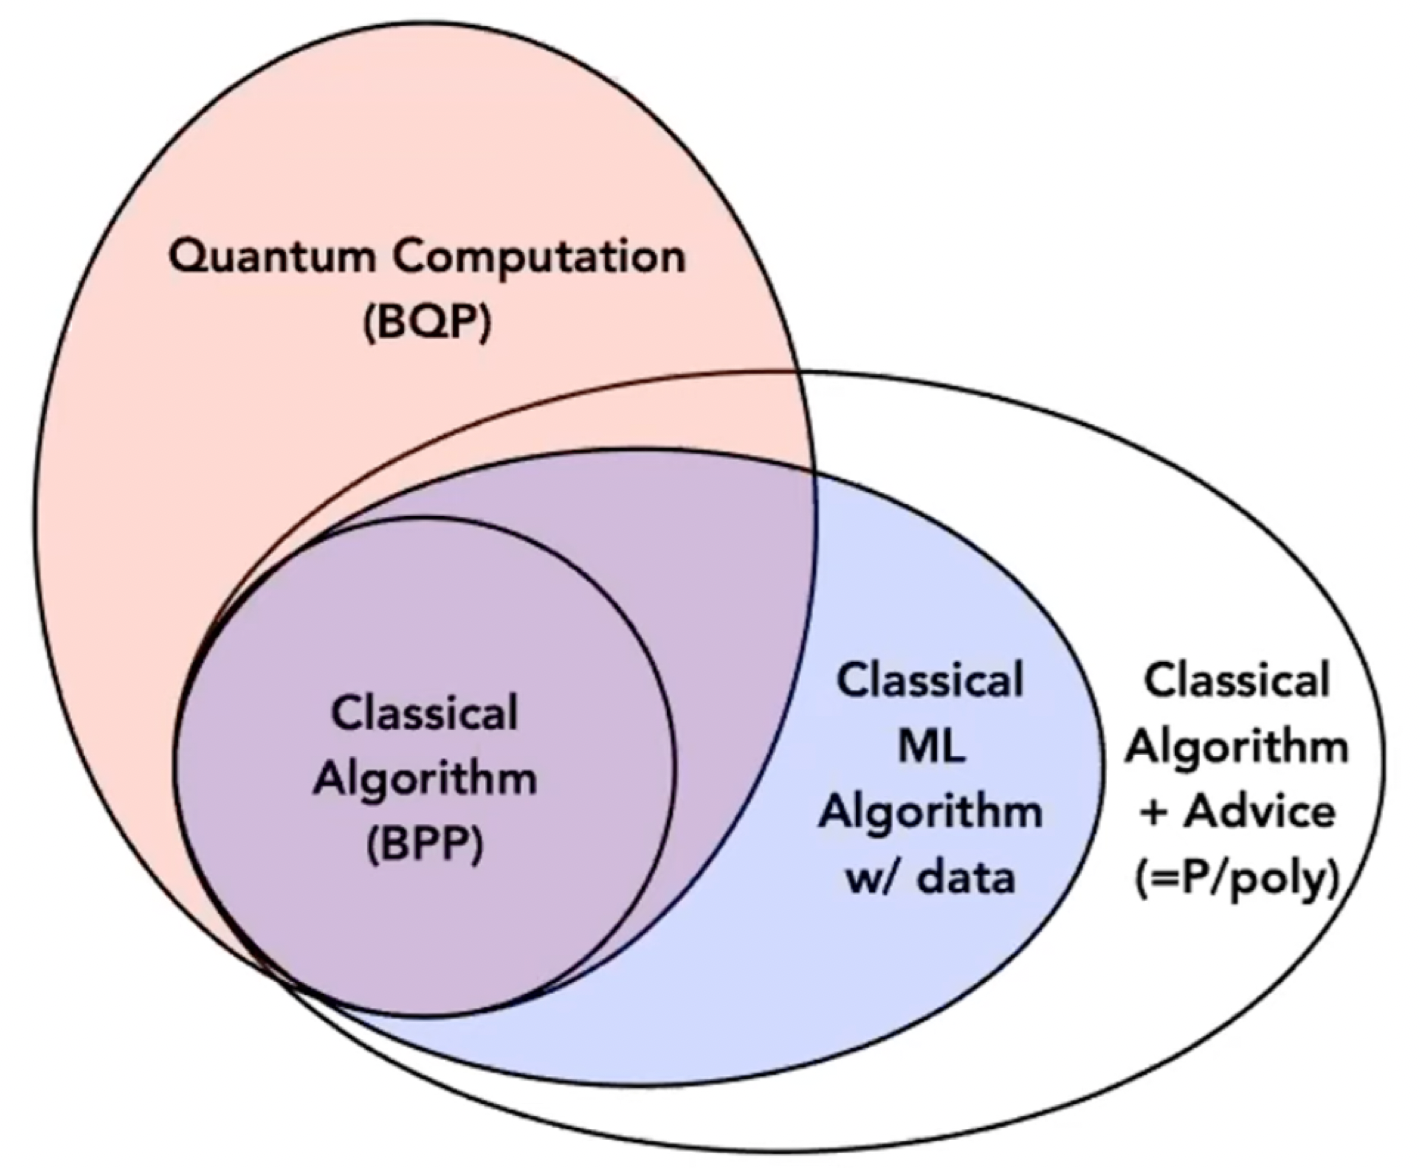
\includegraphics[scale=.2]{data.png}
% 	% 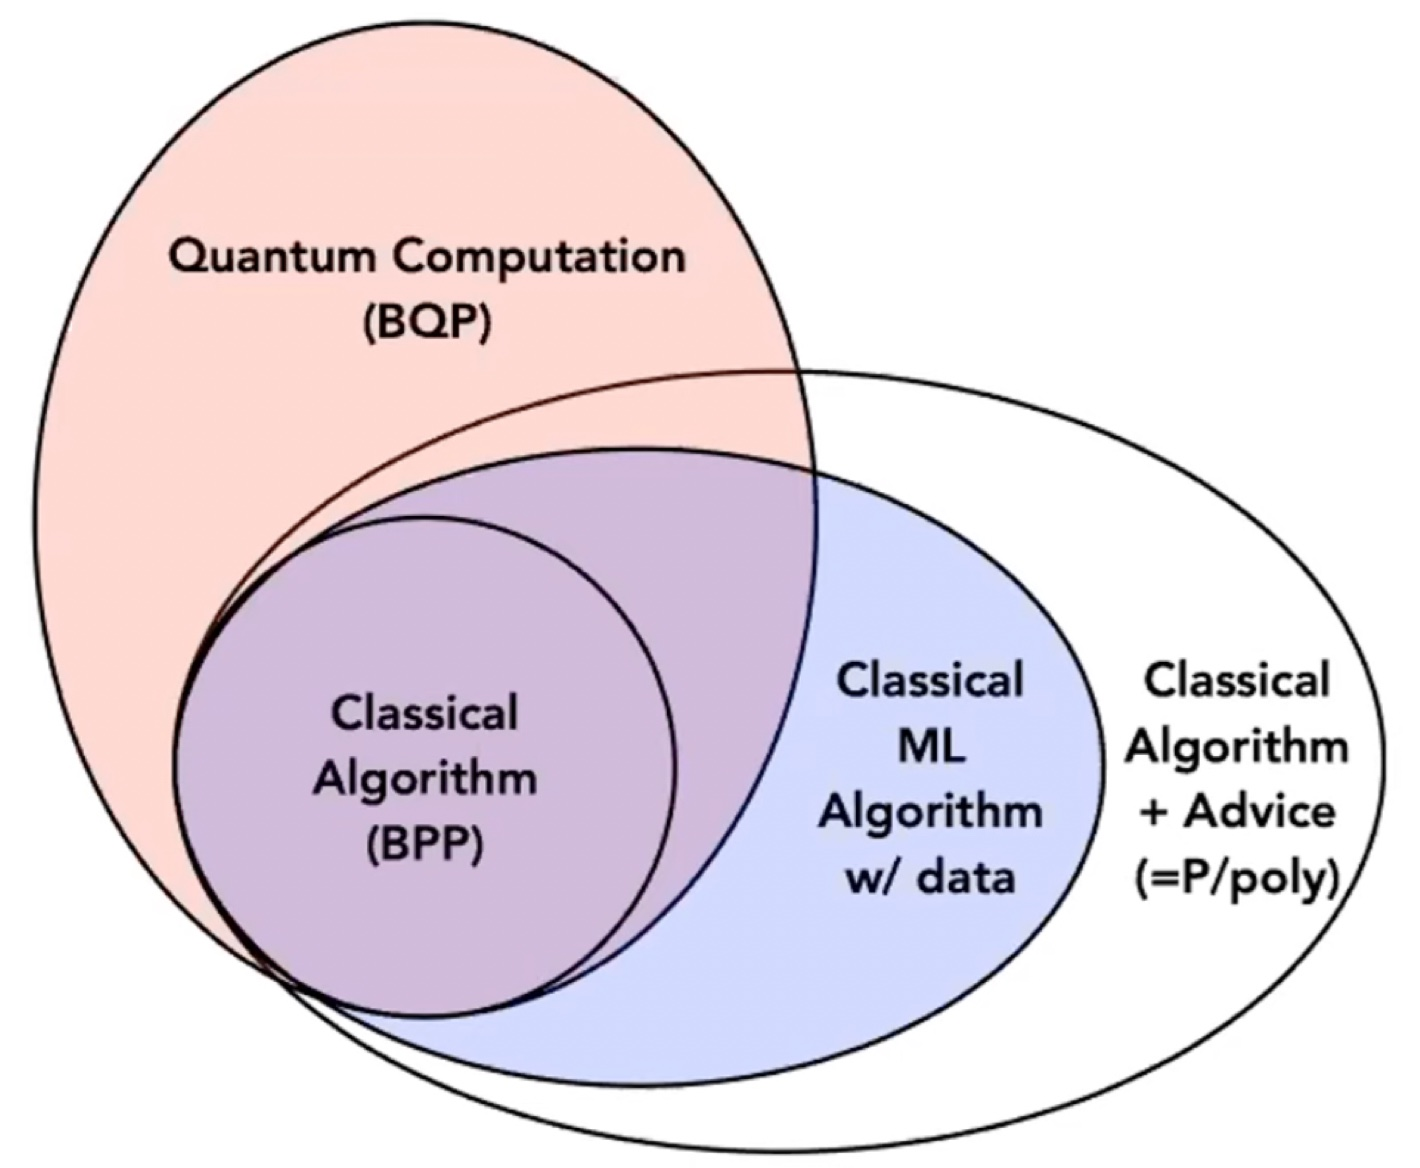
\includegraphics[width=.35\linewidth]{data.jpg}
% 	\caption{computational model powered by training data}
% \end{figure}

% \begin{proposition}[\cite{huangPowerDataQuantum2021}]
% 	exist quantum advantage in machine learning (not significant, practical)	...
% 	discrete log, factoring...
% \end{proposition}
% \begin{theorem}[informal \cite{huangPowerDataQuantum2021}]
% 	data learning
% 	\begin{itemize}
% 		\item machine learning (strictly) more powerful than BPP
% 		\item exist quantum advantage in machine learning (not significant, practical)
% 	\end{itemize}
% \end{theorem}

% \subsubsection{Estimate entanglement witness by (quantum) machine learning}
% though, that while there is no large advantage in query complexity, a substantial quantum advantage in computational complexity is possible.
The task of estimating expectation value can also be achieved efficiently by machin learning with training data \cite{gaoEfficientRepresentationQuantum2017} \cite{torlaiManybodyQuantumState2018} \cite{huangPowerDataQuantum2021} \cite{huangProvablyEfficientMachine2022} \cite{zhuFlexibleLearningQuantum2022}.
% The quantum ML algorithm accesses the quantum channel $\mathcal{E}_\dm$ multiple times to obtain multiple copies of the underlying quantum state $\dm$. Each access to $\mathcal{E}_\dm$ allows us to obtain one copy of $\dm$. Then, the quantum ML algorithm performs a sequence of measurements on the copies of $\dm$ to accurately predict $\Tr(P_{\vbx} \dm ), \forall \vbx \in \qty{ I, X, Y, Z }^n$.
Huang et. al rigorously show that, for any quantum process $\mathcal{E}$, observables $\ob$, and distribution $\mathcal{D}$, and for any quantum ML model, one can always design a classical ML model achieving a similar average prediction error such that $N_C$ (number of experiments?) is larger than $N_Q$ by at worst a small polynomial factor.
In contrast, for achieving accurate prediction on all inputs $\Tr(\dm\pob_{\sigma} ), \forall \sigma \in \qty{ I, X, Y, Z }^n$, exponential quantum advantage is possible.
\begin{theorem}[\cite{huangInformationtheoreticBoundsQuantum2021}]\label{thm:quantum_ml_estimate_bound}
% 	For $M$ Pauli opertors, there is a (quantum) procedure estimate every expectation value $\Tr(P_x \dm),\forall i=1,\dots,M$ within error $\epsilon$ under probability at least $1-\delta $ by performing POVM measurements on $\bigO(\log(M/\delta)\epsilon^{-4})$ copies of the unknown quantum state $\dm$.
	To predict expectations of all Pauli observables of an $n$-qubit system $\dm$, classical ML models require $2^{\Omega(n)}$ copies of $\dm$ , 
	there is a quantum ML model using only $\bigO(n)$ copies.
	\footnote{
		$\bigO(\log(M/\delta)\epsilon^{-4})$ copies of the unknown quantum state $\dm$.
		($M=4^n$ implies linear copy for full tomography???)
	}
	\footnote{
		% \cite{huangPowerDataQuantum2021}
		the required amount of training data scales badly with $\epsilon$. This unfortunate scaling is not a shortcoming of the considered ML algorithm, but a necessary feature.
	}
\end{theorem}
\begin{table}[!ht]
	\centering
	% \begin{tabular}{c|c|c}
	\begin{tabular}{c|c}
		& circuit/sample complexity \\
		\hline
		\nameref{prm:shadow_tomography} & \cref{thm:shadow_tomography} (exponential circuit?) \\  
		classical shadow & \cref{thm:classical_shadow} (experiment friendly)  \\
		% derandomized CS &  better performance \\  
		% quantum circuit  &  \cref{thm:multivariate_trace} (c-depth?)  ? \\  
		classical/quantum ML  &  % \cref{thm:quantum_vs_classical} 
		\cref{thm:quantum_ml_estimate_bound} (quantum advantage?)\\  
		\hline
	\end{tabular}
	\caption{complexity (measures) of different expectation estimation methods}
\end{table}
	
% \subsection{Quantum trace (kernel) estimation by quantum circuits}


% \subsubsection{Variational trace estimate (direct)}
% \begin{theorem}
% 	On quantum computers, evaluating the trace distances is probably hard since even judging whether $\dm$ and $\dm'$ have large or small trace distance is known to be QSZK-complete \cite{watrousQuantumComputationalComplexity2008}, where QSZK (quantum statistical zero-knowledge) is a complexity class that includes BQP (bounded-error quantum polynomial time).
% 	% Variational Quantum Algorithms for Trace Distance and Fidelity Estimation
% \cite{chenVariationalQuantumAlgorithms2022}
% \end{theorem}

% \subsection{Theoretic upper bounds and lower bounds}
% \cite{huangPredictingManyProperties2020}
% \cite{huangInformationtheoreticBoundsQuantum2021}
% \cite{huangPowerDataQuantum2021}
% \cite{aaronsonShadowTomographyQuantum2018}
% \cite{liuRigorousRobustQuantum2021}

% \begin{table}[!ht]
% \centering
% \begin{tabular}{c|c|c|c|c}
% 	& gate/depth/computation & measurements/samples & query? & input/unknown? \\  
% 	% necessary?sufficient
% 	\hline
% 	% \nameref{prm:full_tomography} & & N/A & $\bigO$, Holevo bound $\Omega$ & \\  
% 	\nameref{prm:shadow_tomography} & exp circuit? & \cref{thm:shadow_tomography} & N/A & unknown \\  
% 	% indirect? direct (no prior), promise & & & & \\  
% 	% promise (low-rank?), partial, decision? & & & & \\  
% 	\nameref{def:entanglement_witness} & N/A &  \cref{thm:entanglement_witness_gme} (constant?) & convex?\cite{chakrabartiQuantumAlgorithmsLower2020} & known \\  
% 	\nameref{def:classical_shadow}  & N/A & \cref{thm:classical_shadow_upper,thm:classical_shadow_lower} & N/A & unknown? \\  
% 	C. ML + C. \nameref{def:entanglement_witness} ansatz  & ?? & Q. advantage \cref{thm:quantum_vs_classical} & N/A & unknown \\  
% 	QML. \nameref{def:entanglement_witness} ansatz  & ?? & \cref{thm:quantum_ml_estimate_bound} & N/A & unknown \\  
% 	Q. \nameref{def:entanglement_spectroscopy} &  \cref{thm:multivariate_trace} (c-depth?) & & property test \cite{montanaroSurveyQuantumProperty2018} & unknown\\  
% 	% SVM + quantum kernel estimation &  & &  & ??\\  
% 	\hline
% \end{tabular}
% \caption{complexity (different measures) of different methods}
% \end{table}


% \begin{table}[!ht]
% 	\centering
% 	\begin{tabular}{c|c|c}
% 		& accuracy & complexity \\
% 		\hline
% 		linear SVM & & \\  
% 		kernel SVM & & \\  
% 		Neural network & & \\  
% 		neural kernel & & \\  
% 		quantum kernel & & \\  
% 		\hline
% 	\end{tabular}
% 	\caption{machine learning methods}
% \end{table}

% \subsubsection{Separations (complexity)}
% contrived problem (engineered dataset)? for exponential speedup

% \subsubsection{Obstacles (practical)}

% quantum advantages:
% \begin{itemize}
% 	\item no input encoding problem? \cite{tangQuantumPrincipalComponent2021} in most quantum machine learning algorithm.
% 	\item contrived problem (engineered dataset)? for exponential speedup
% 	% \item convex body query? complexity
% \end{itemize}
% obstacles: (i)

\section{Numerical simulation}\label{sec:numerical_simulation}
\subsection{Dataset preparation and states generation}\label{sec:data}
We generate quantum state samples, construct quantum circuits, and manipulate quantum objects numerically by QuTiP library \cite{johanssonQuTiPPythonFramework2013} \cite{liPulselevelNoisyQuantum2022}.
We generate multi-partite entangled states (synthetic data) including: Bell states, 3-qubit GHZ and W states, 4-qubit graph (1D cluster) state, see \cref{fig:sample_data} for examples.
% \begin{equation}
% 	\cos(\theta) \ket{00} + \sin(\theta)e^{\ii \phi} \ket{11}
% 	,\;
% 	\cos(\theta) \ket{01} + \sin(\theta)e^{\ii \phi} \ket{10}
% \end{equation}
\begin{figure}[!ht]
	\centering
	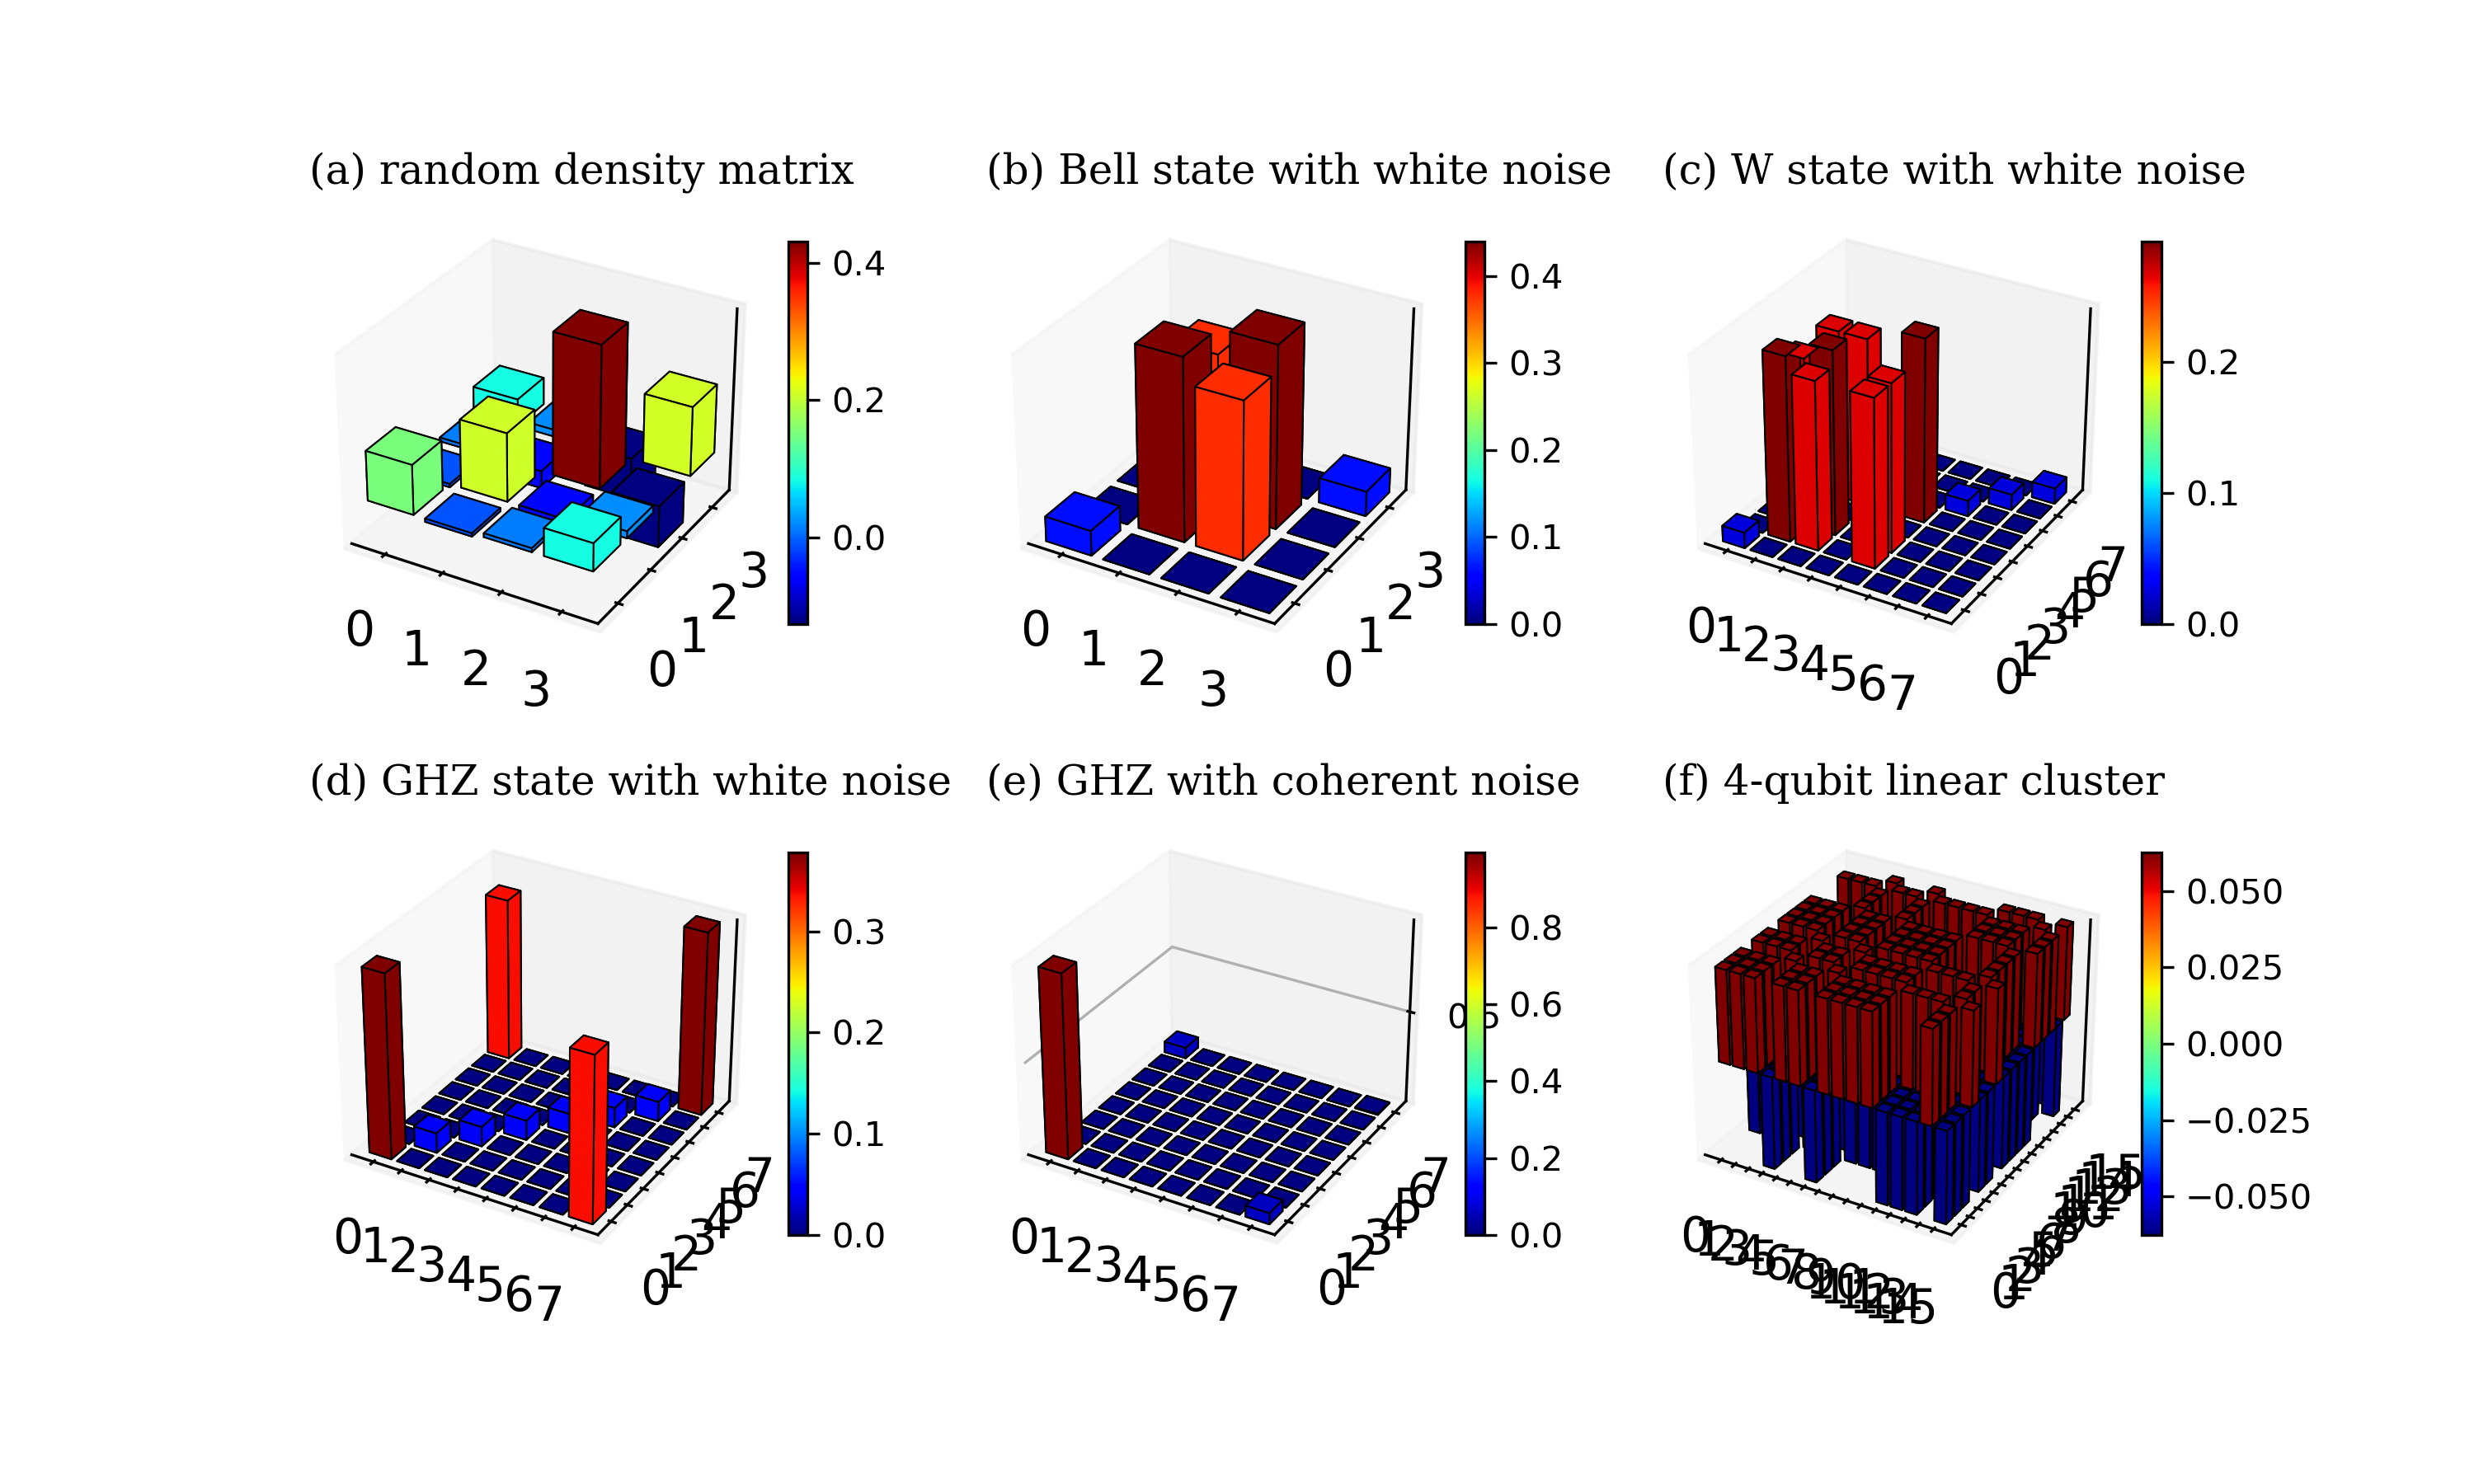
\includegraphics[width=.9\linewidth]{./Code/dataset_sample_3x2.png}
% 		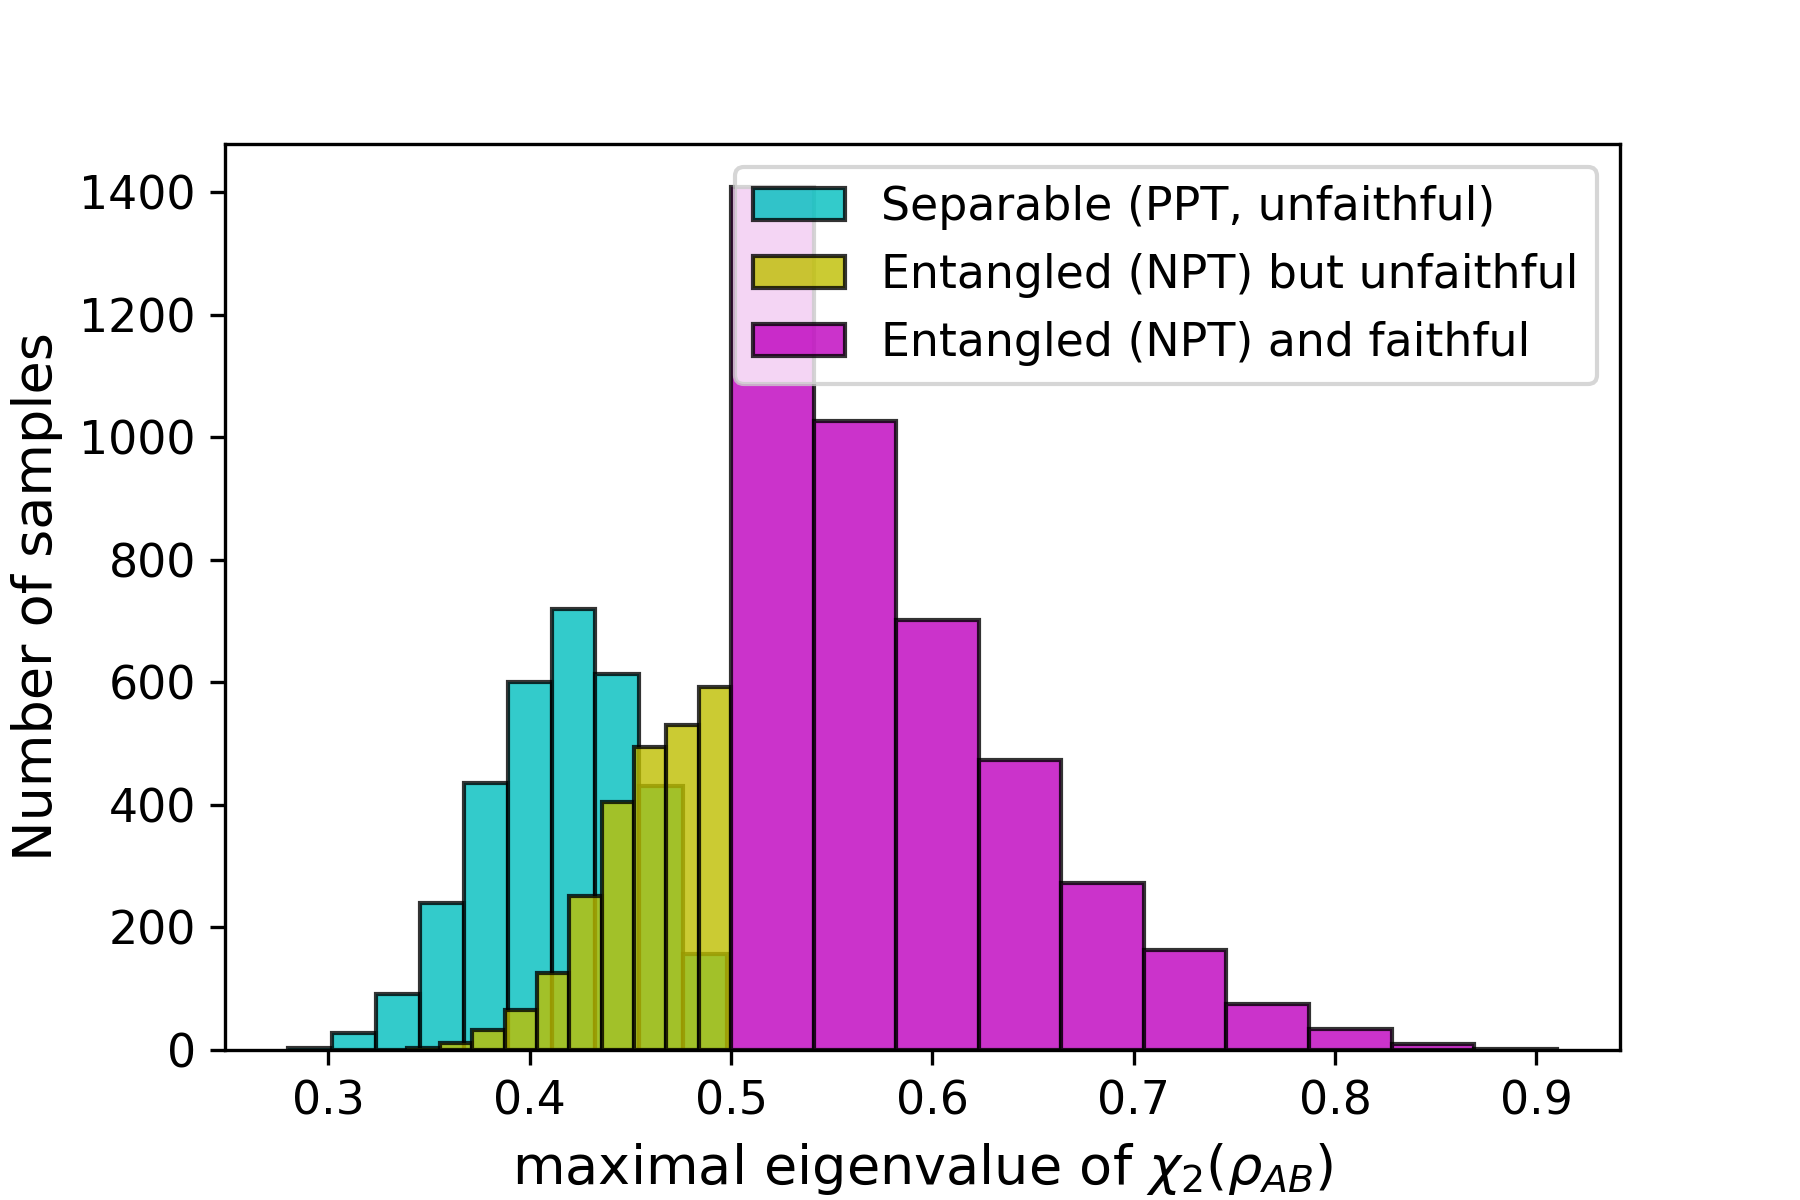
\includegraphics[width=.9\linewidth]{./Code/faithfulness_2_qubit.png}
	% \caption{PPT criterion (2-qubit random density matrix)}
	\caption{Data praparation: (a) random 2-qubit density matrix; (b) Bell state with white noise; (c) 3-qubit W state with white noise; (d) 3-qubit GHZ state with white noise; (e) GHZ state with coherent noise; (f) 4-qubit linear cluster.}
	\label{fig:sample_data}
\end{figure}
In contrast to entangled states, we generate random separable states for different number of qubits by tensoring random density matrices of subsystems.
For example,
2-qubit: bipartite $\rho_A\otimes \rho_B$ where $\rho_A$ and $\rho_B$ are random density matrices (sampled by Haar measure);
3-qubit pure states: $\dm_A\otimes \dm_{BC}$, $\dm_C\otimes \dm_{AB}$, and $\dm_B\otimes \dm_{AC}$.
For different noise channels: white noise according to \cref{eq:white_noise}, coherent noise according to \cref{eq:coherent_noise}.


\subsection{Classification accuracy and comparison}

For the machine learning part, we make use of scikit-learning package \cite{pedregosaScikitlearnMachineLearning2011} to train SVM with the radial basis function (RBF) kernel.

% \subsubsection{Hyperparameters and settings}

% \begin{figure}[!ht]
% 	\centering
% 	\includegraphics[width=1\linewidth]{.pdf}
% 	\caption{accuracy VS number of features}
% \end{figure}
% The goal of recursively feature elimination (RFE) is to eliminate non-essential features by recursively considering smaller and smaller subsets of the original features using a greedy algorithm. Initially, RFE takes the SVM we trained and ranks the coefficients by their magnitudes, with the lowest one pruned away; then the model is trained again with the remaining features.
\cref{fig:feature_space} shows the two-dimensional embedding of  2-qubit states (feature space).
The colored shade indicates the decision boundary of our trained classifier (ML witness),
which exhibits that two kinds of data points are clearly classified.
\begin{figure}[!ht]
	\centering
	% 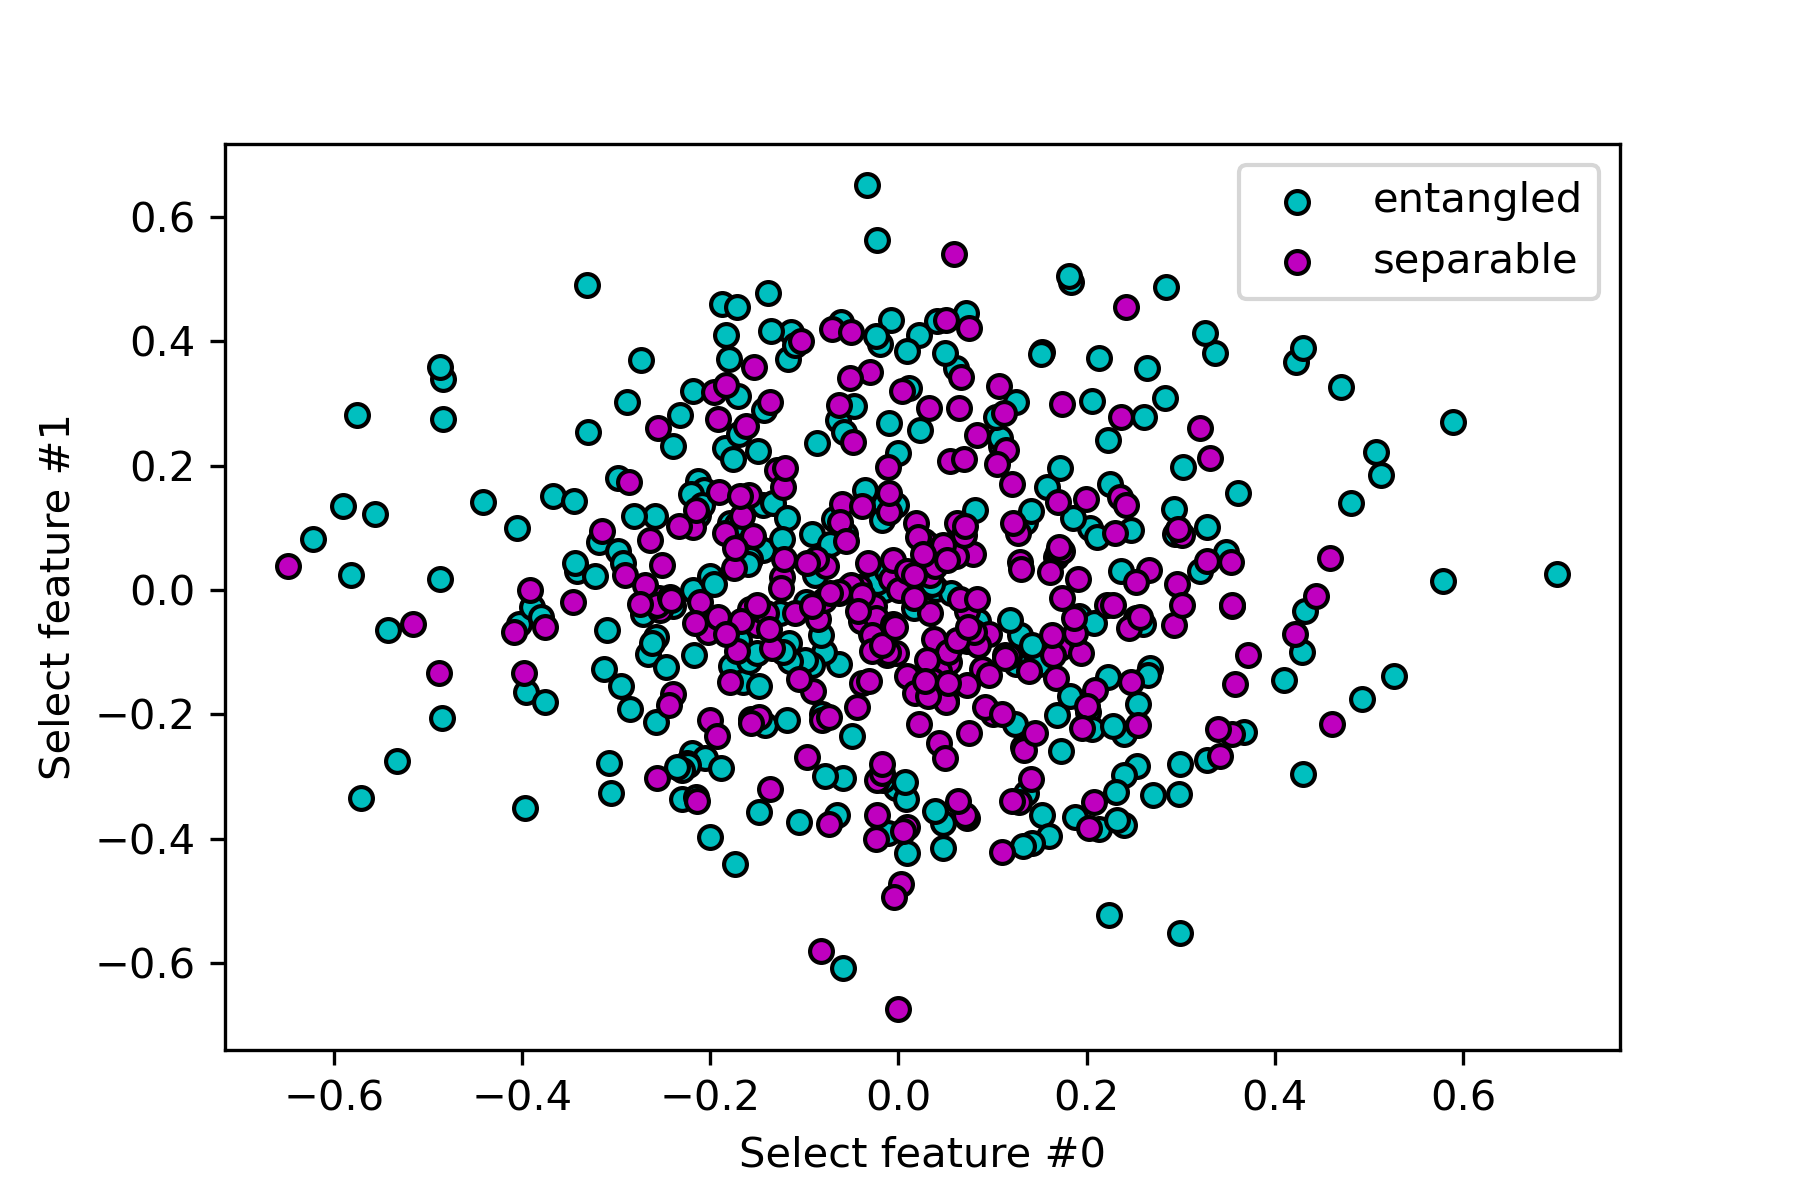
\includegraphics[width=.4\linewidth]{./notebook/feature_space_2.png}
% 	% 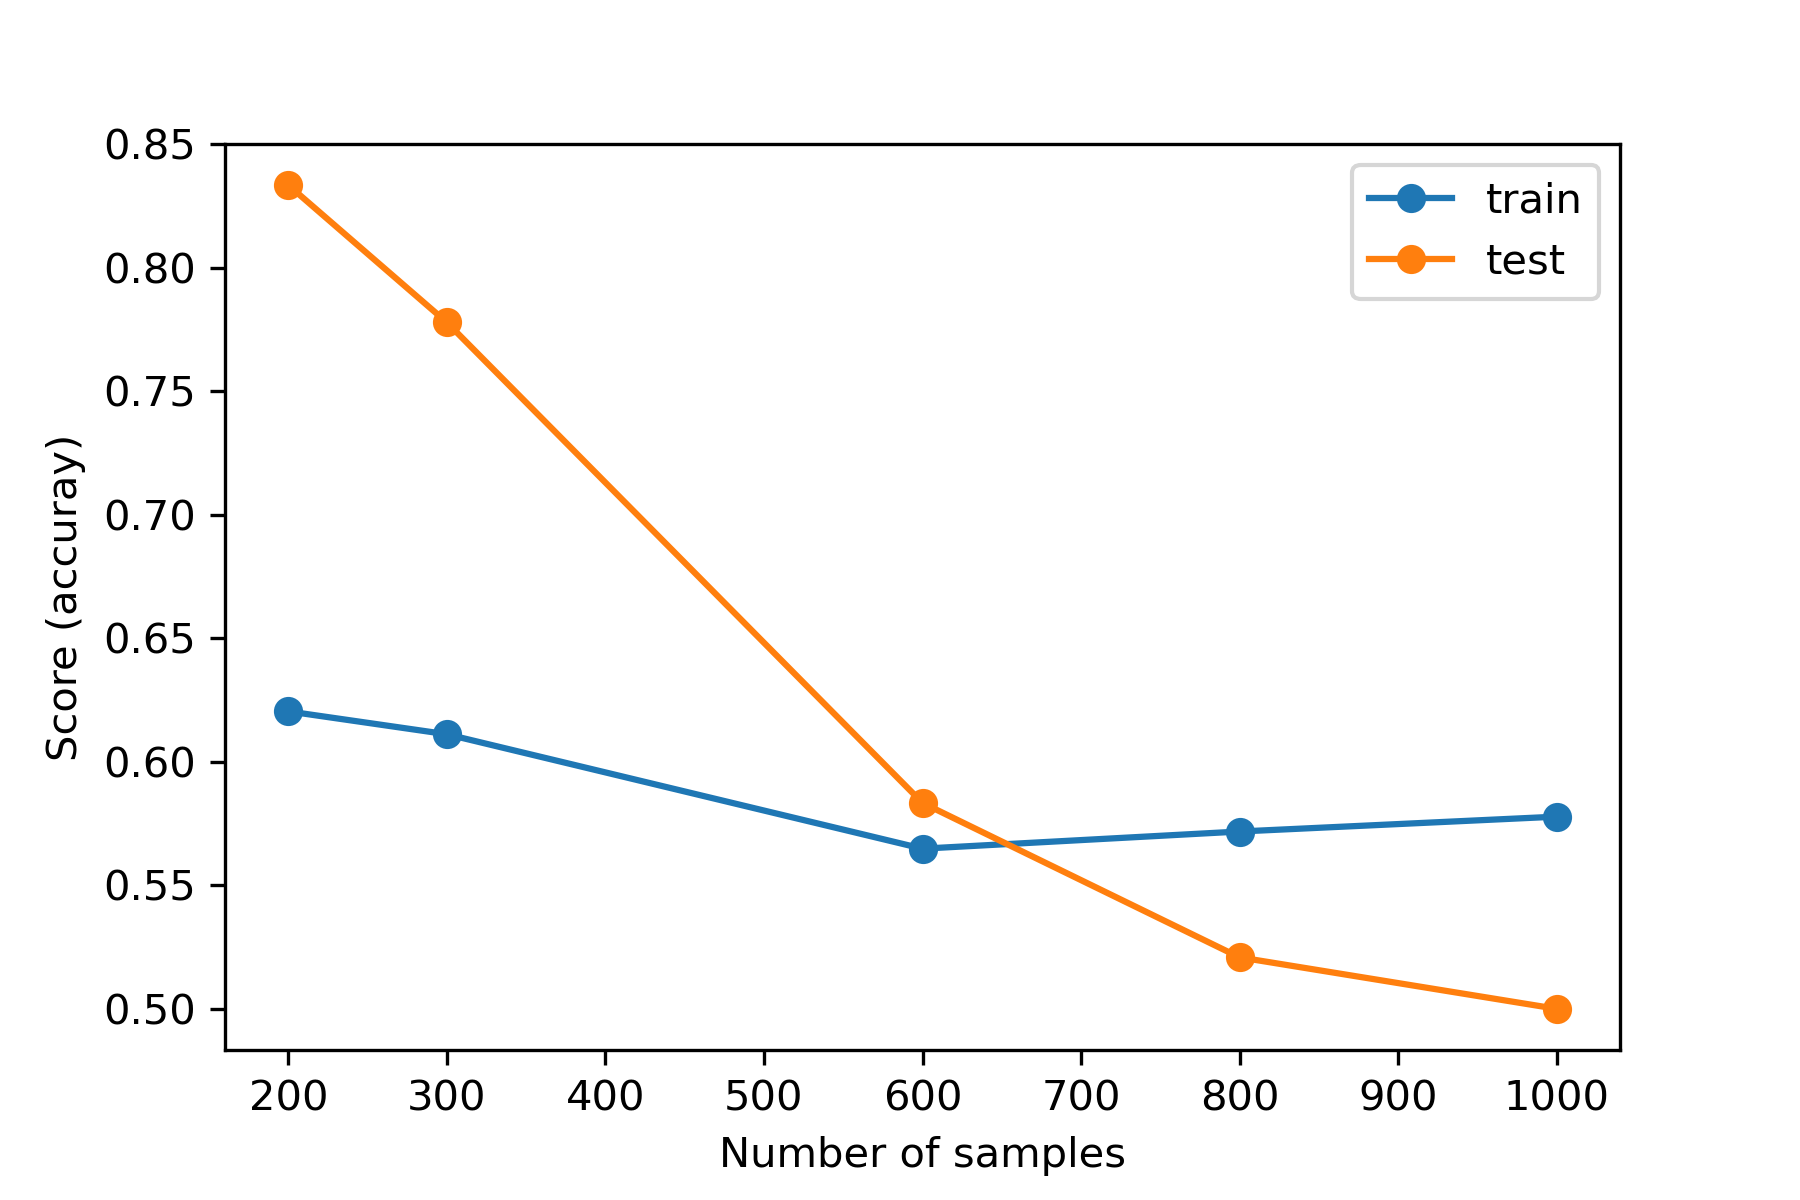
\includegraphics[width=.4\linewidth]{./Code/two_qubit_scores.png}
% 		% 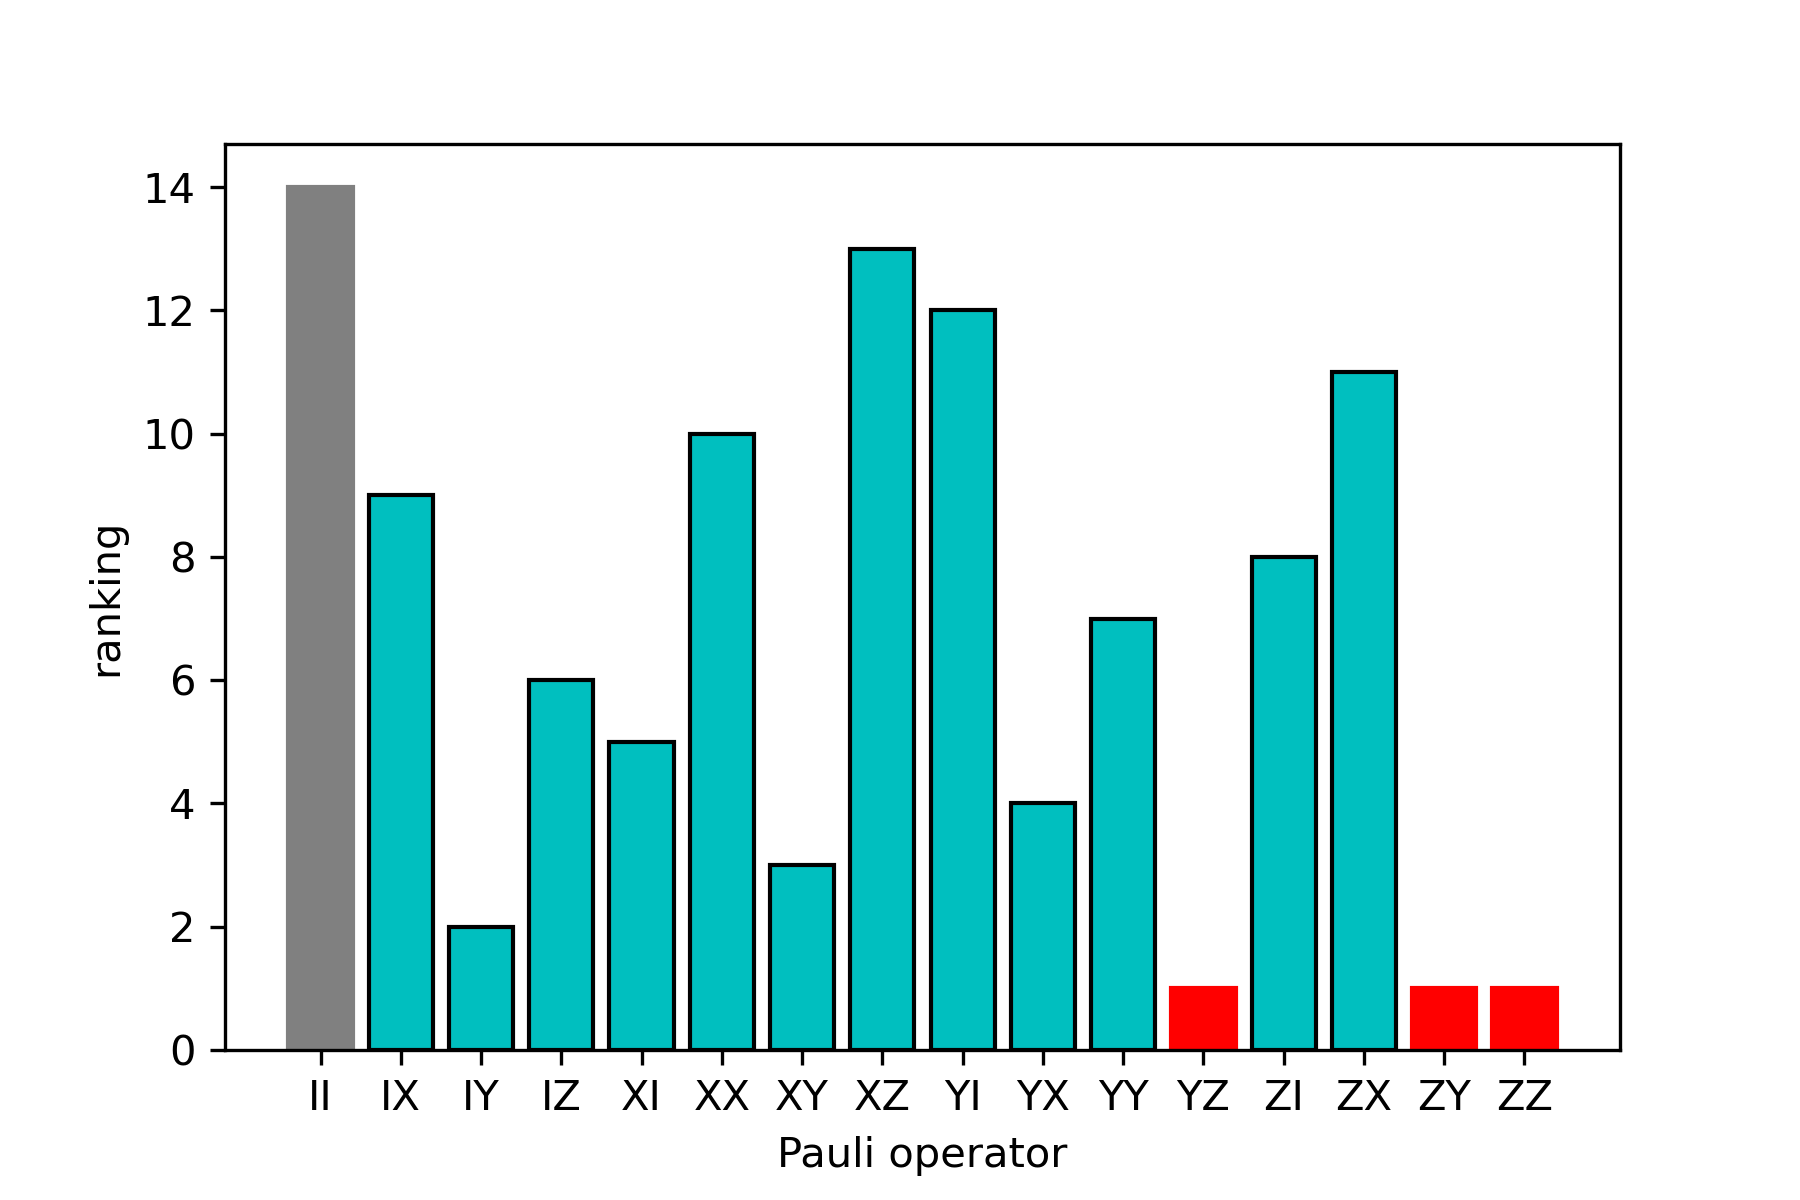
\includegraphics[width=.9\linewidth]{./Code/feature_rank.png}
% 		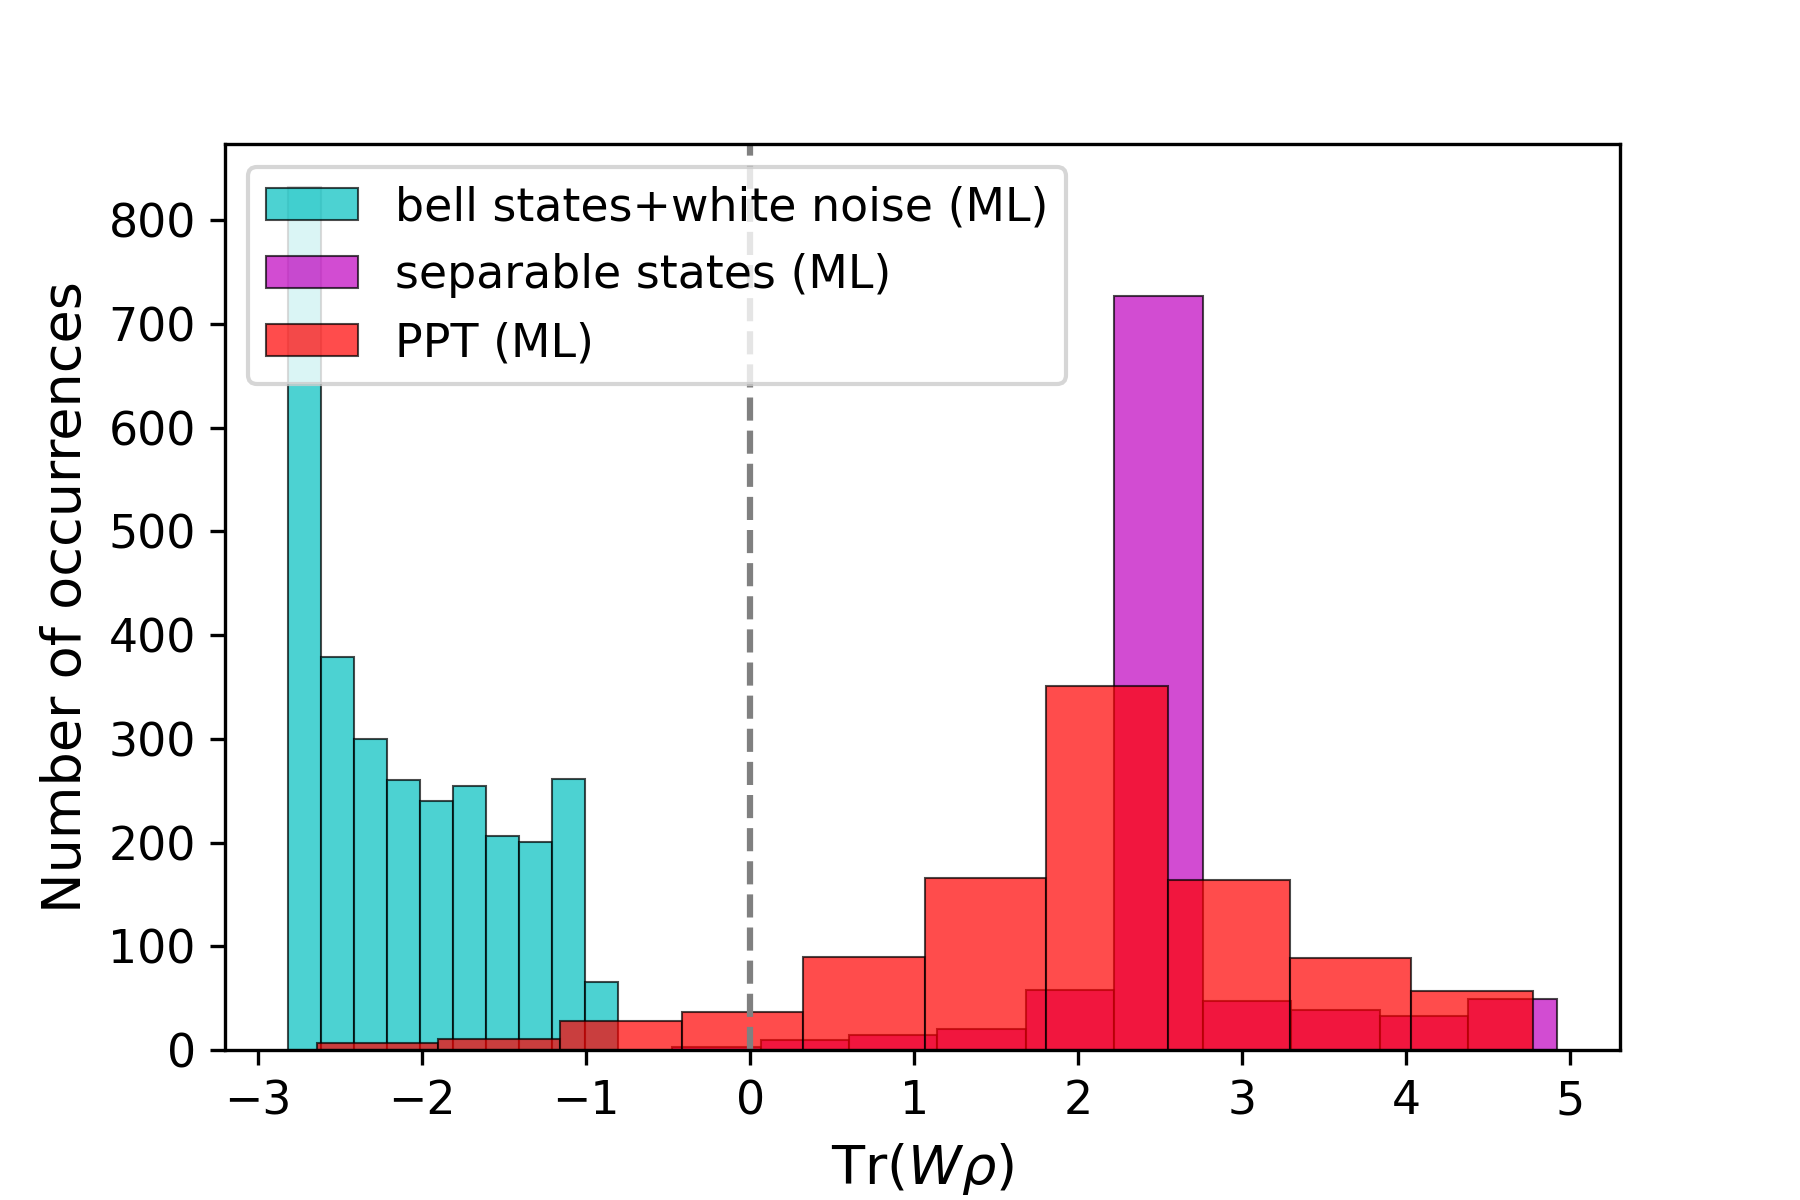
\includegraphics[width=.9\linewidth]{./Code/two_qubit_bell_ml.png}
	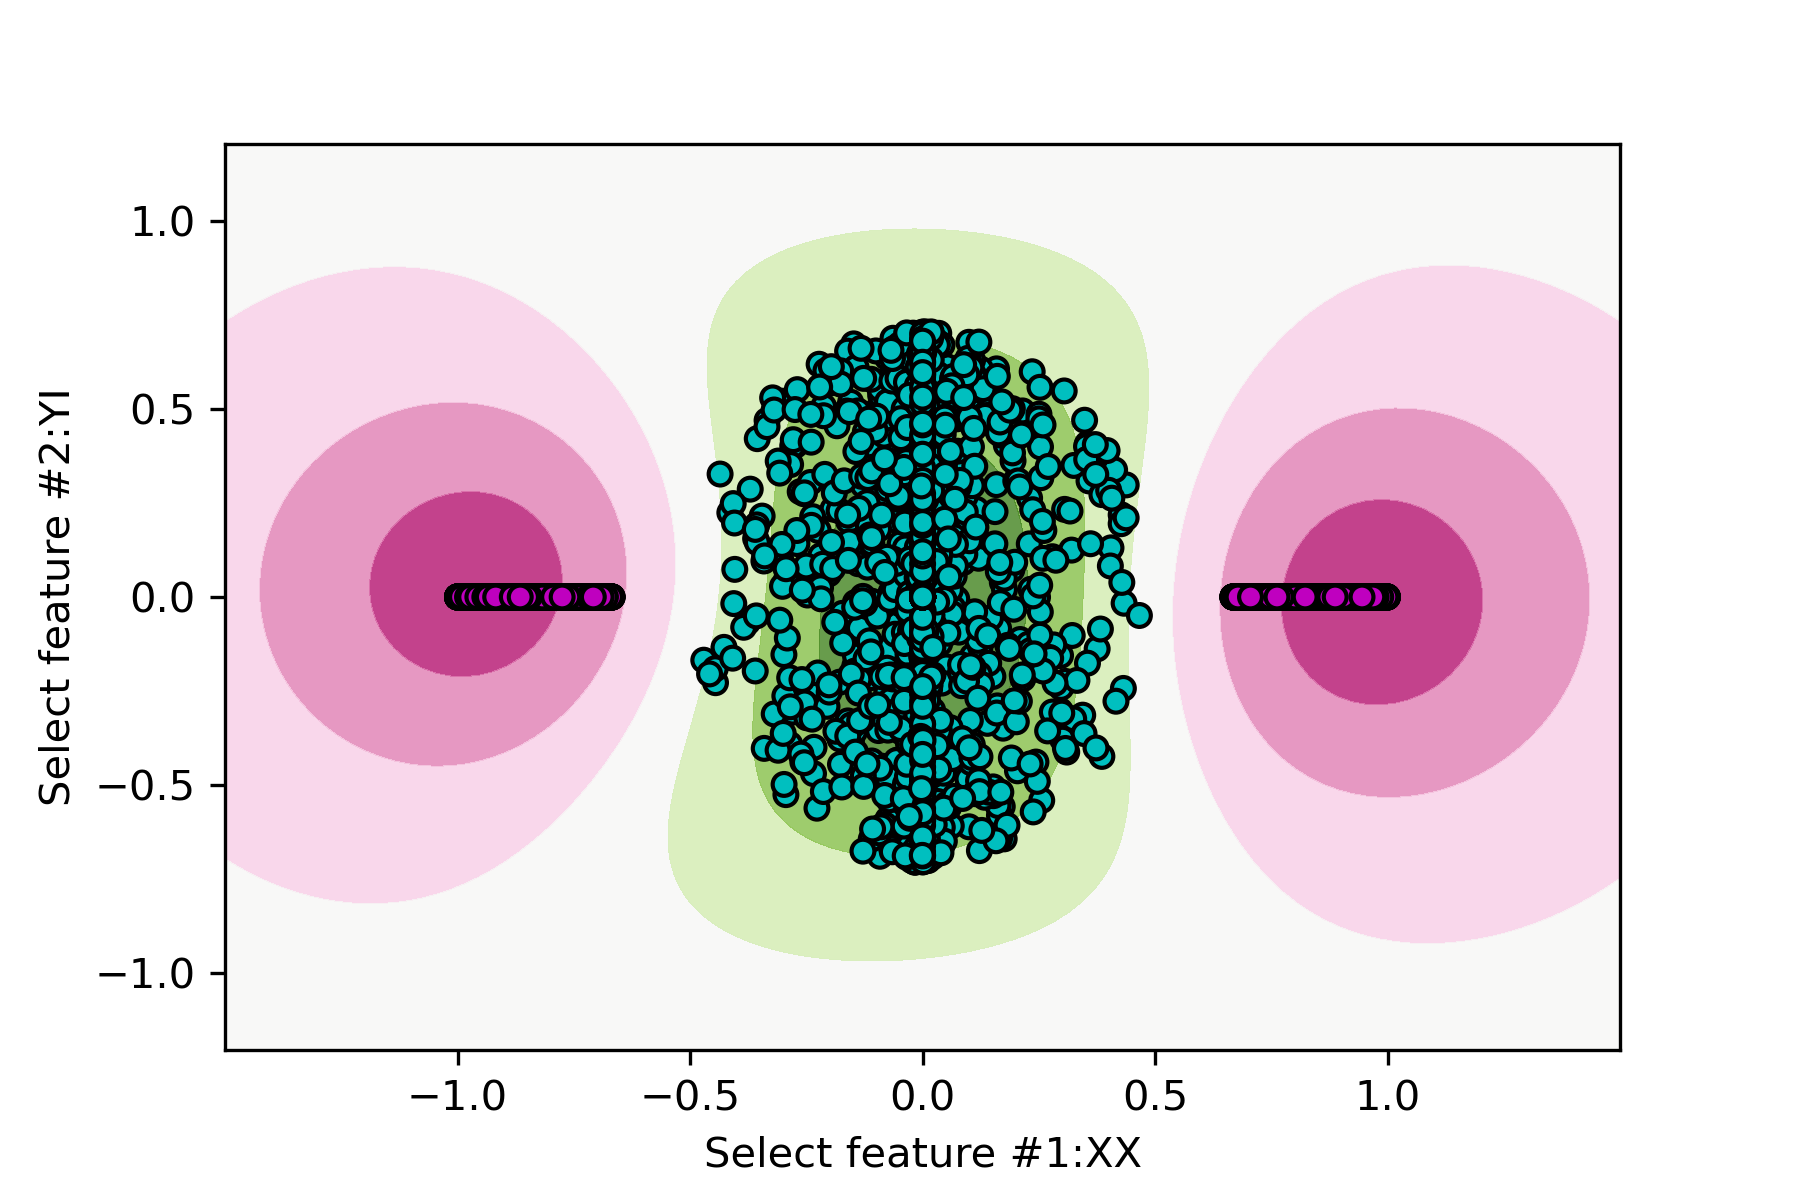
\includegraphics[width=.9\linewidth]{./Code/feature_space_2d.png}
	\caption{two-dimensional embedding (feature space): green dots represent the separable states, while pink one represent entangled Bell states mixed with white noise.}
	% \caption{feature space, recursive feature elimination}
	\label{fig:feature_space}
\end{figure}

% \subsection{Robustness to noise}

% \begin{figure}[!ht]
% 	\centering
% 	% \includegraphics[width=1\linewidth]{.pdf}
% 	\caption{robustness: accuracy VS p noise }
% \end{figure}
\cref{fig:ml_compare} shows that the SVM witness can classify the states that cannot be detected by conventional fidelity witness,
where the noise is randomly (uniform) sampled from $[0,p_{\noise}]$.

% \subsubsection{Results, feature elimination}
% performance of different methods: 
\begin{figure}[!ht]
	% \begin{subfigure}{0.45\textwidth}
	\centering
		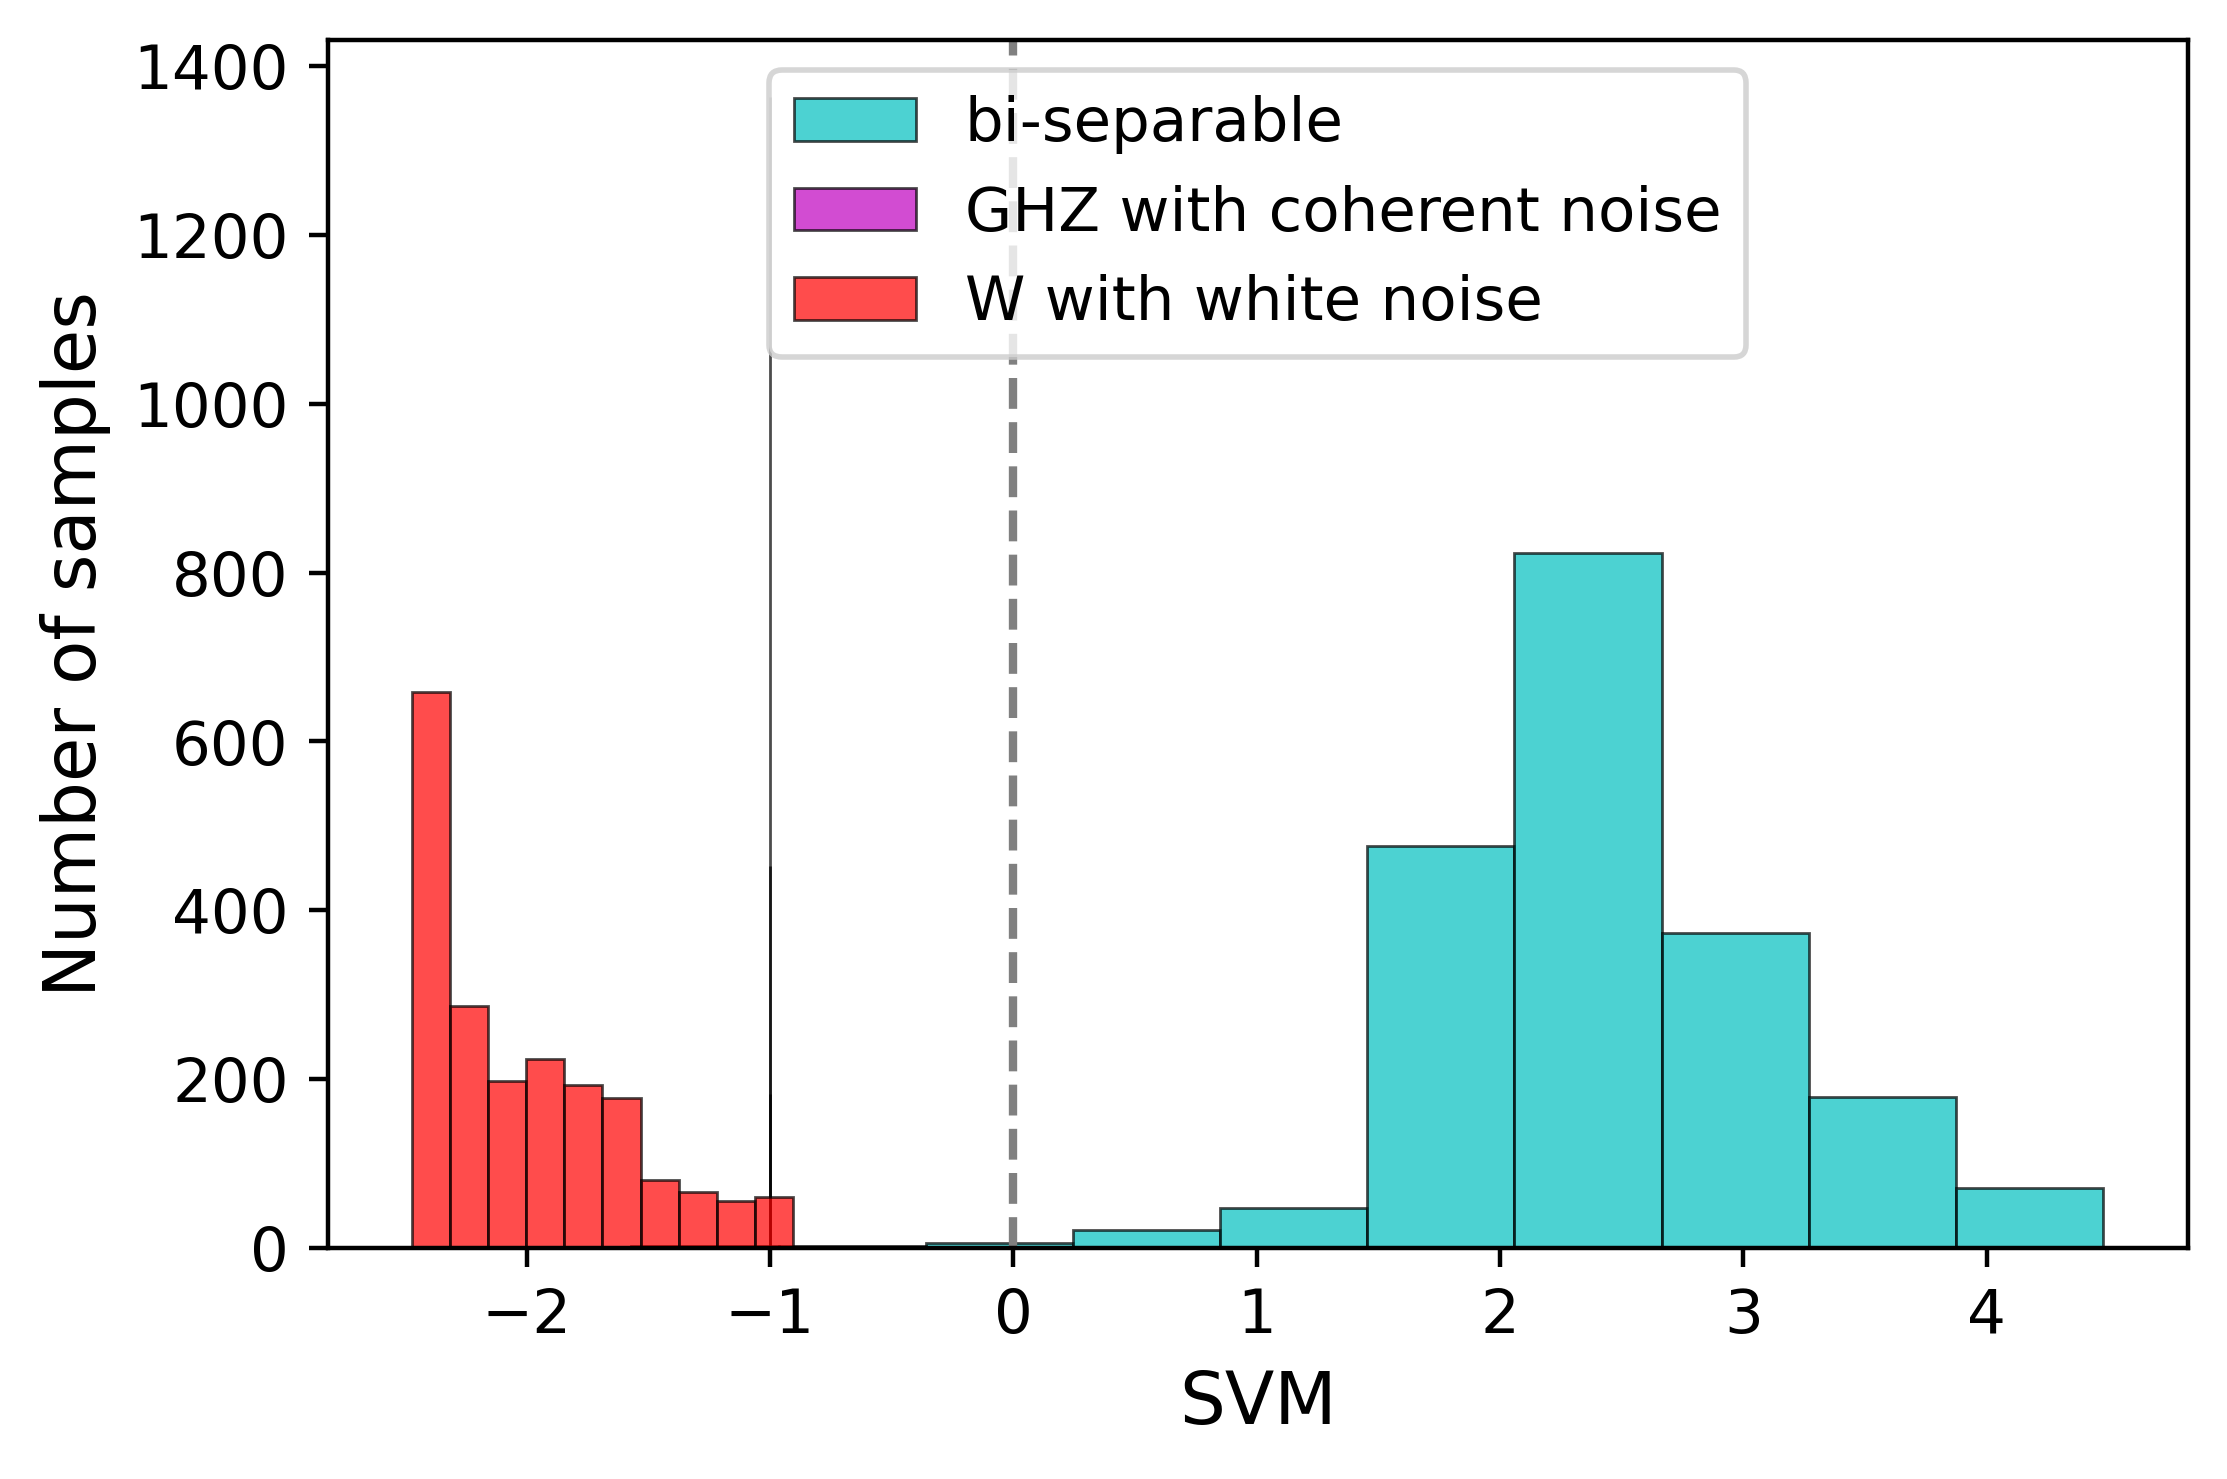
\includegraphics[width=.9\linewidth]{./Code/three_qubit_hist_ML.png}
		% 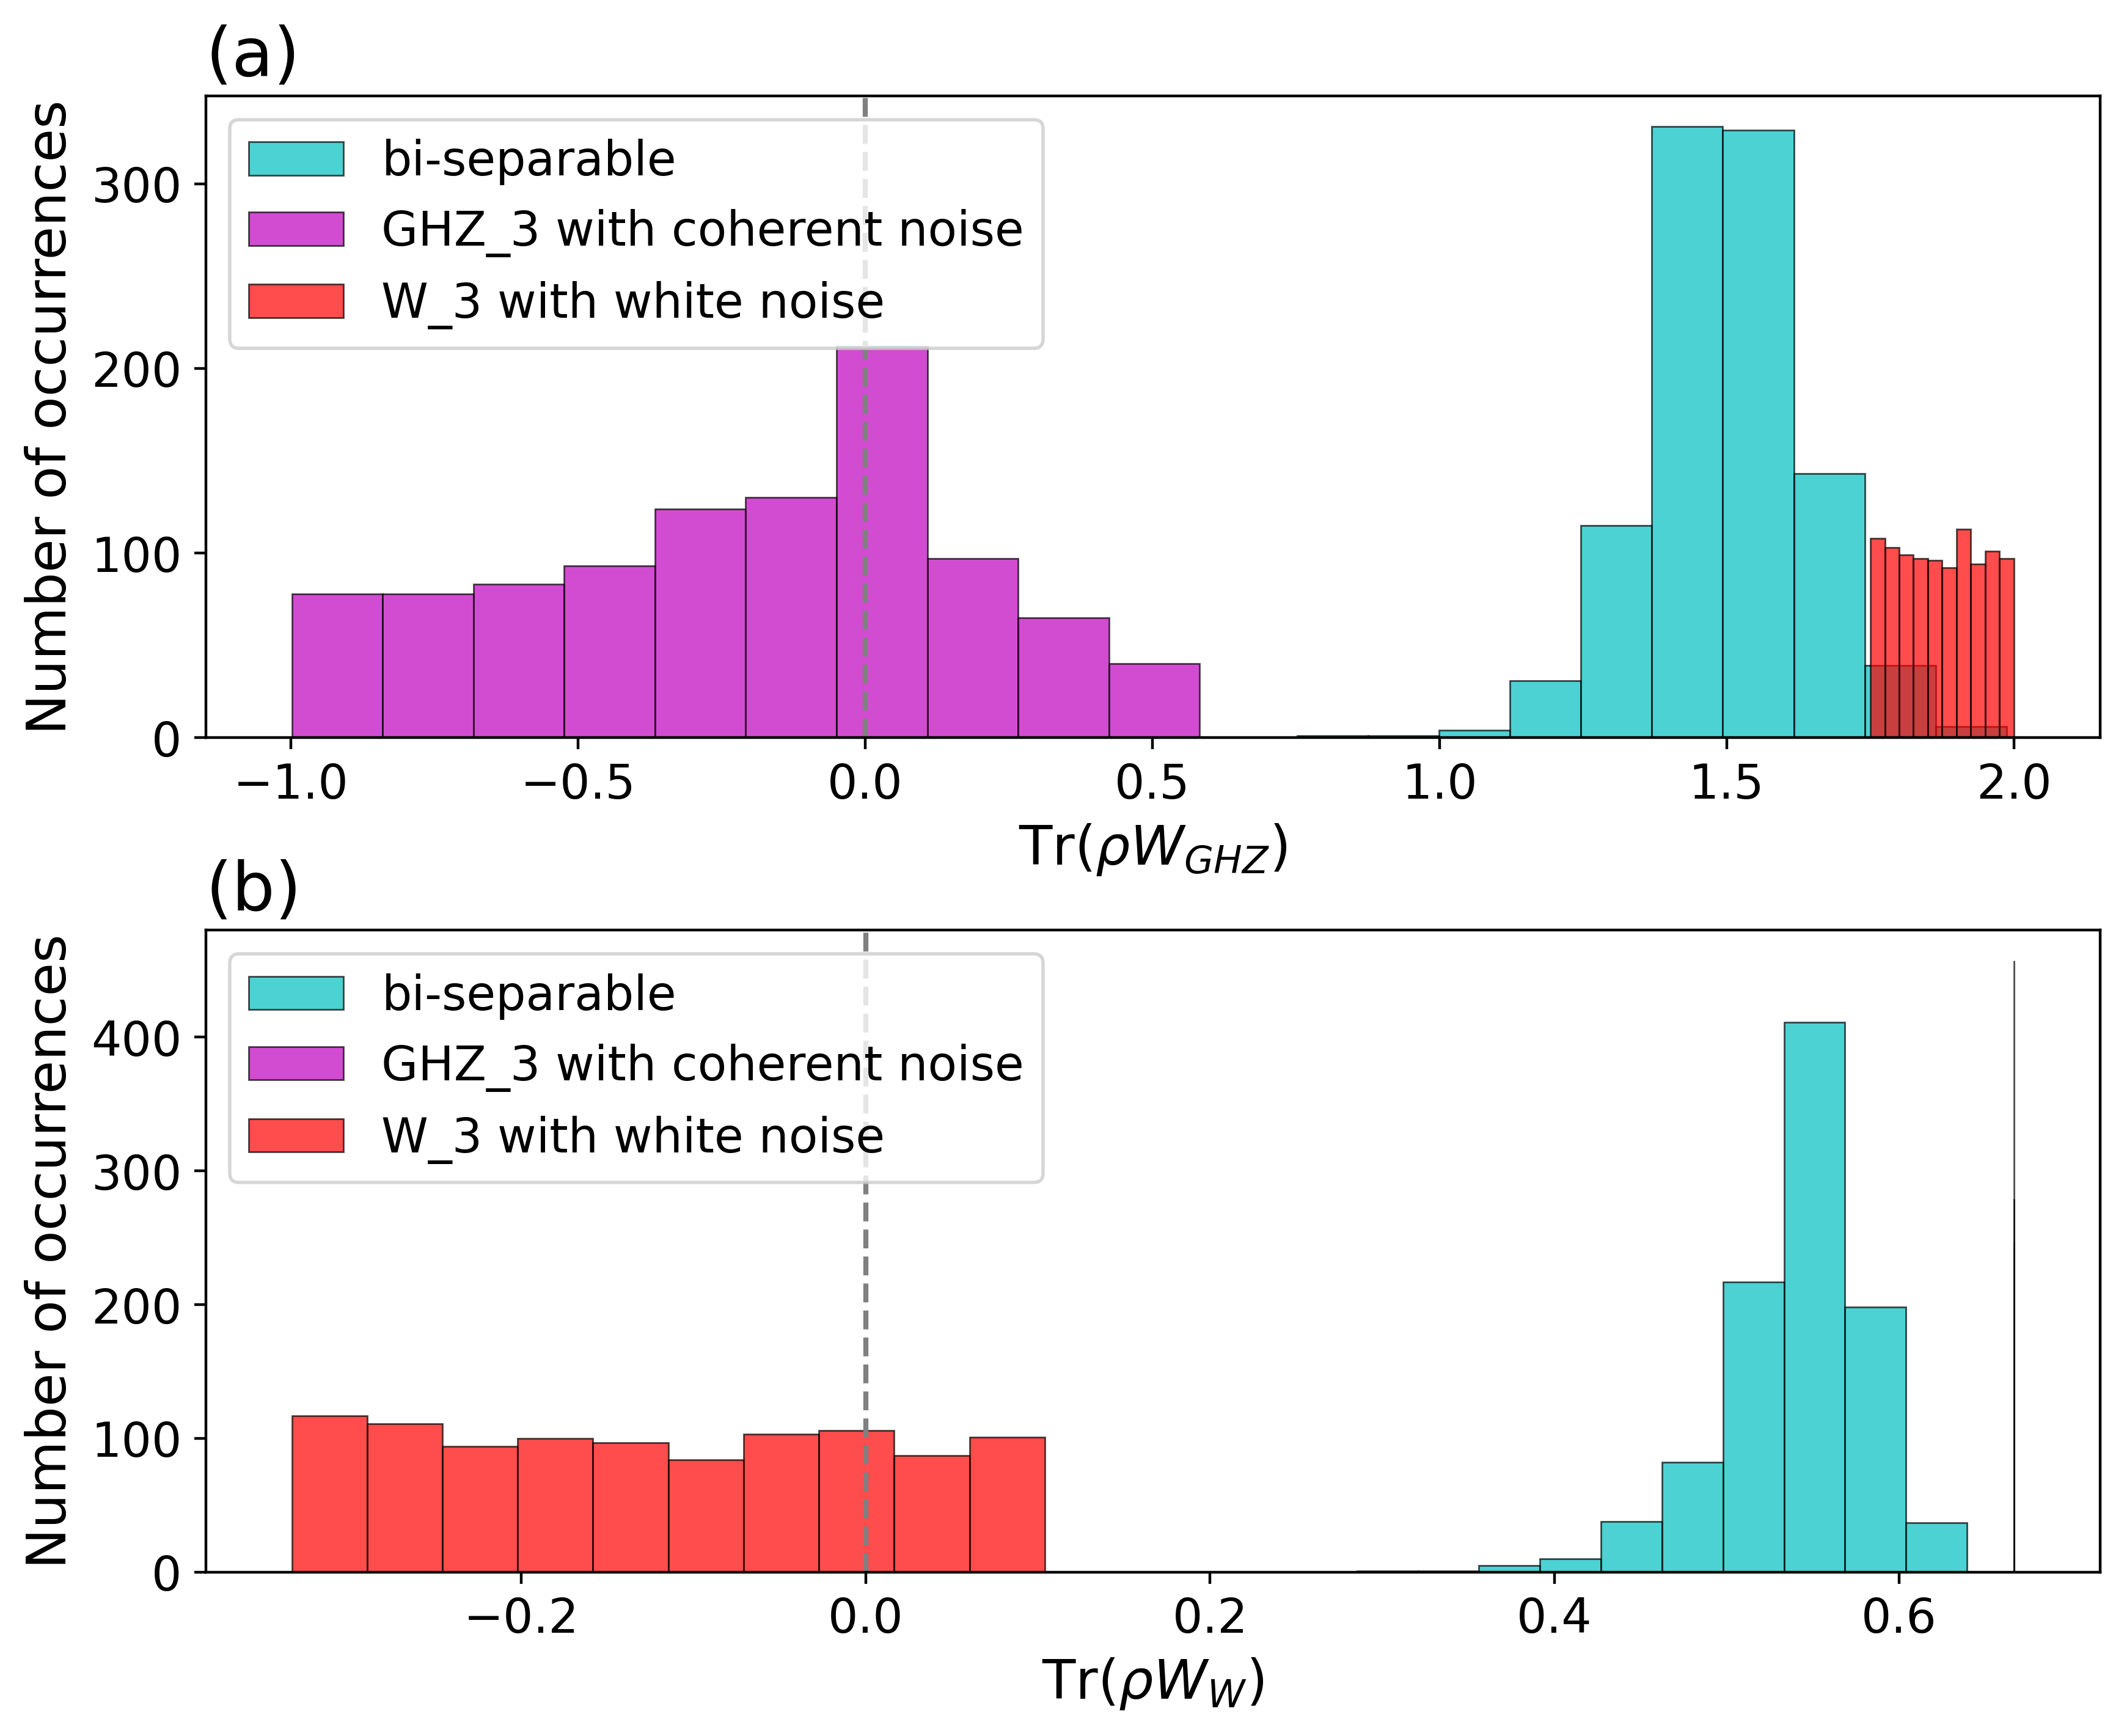
\includegraphics[width=.9\linewidth]{./Code/fidelity_witness_compare_2_long.png}
		% 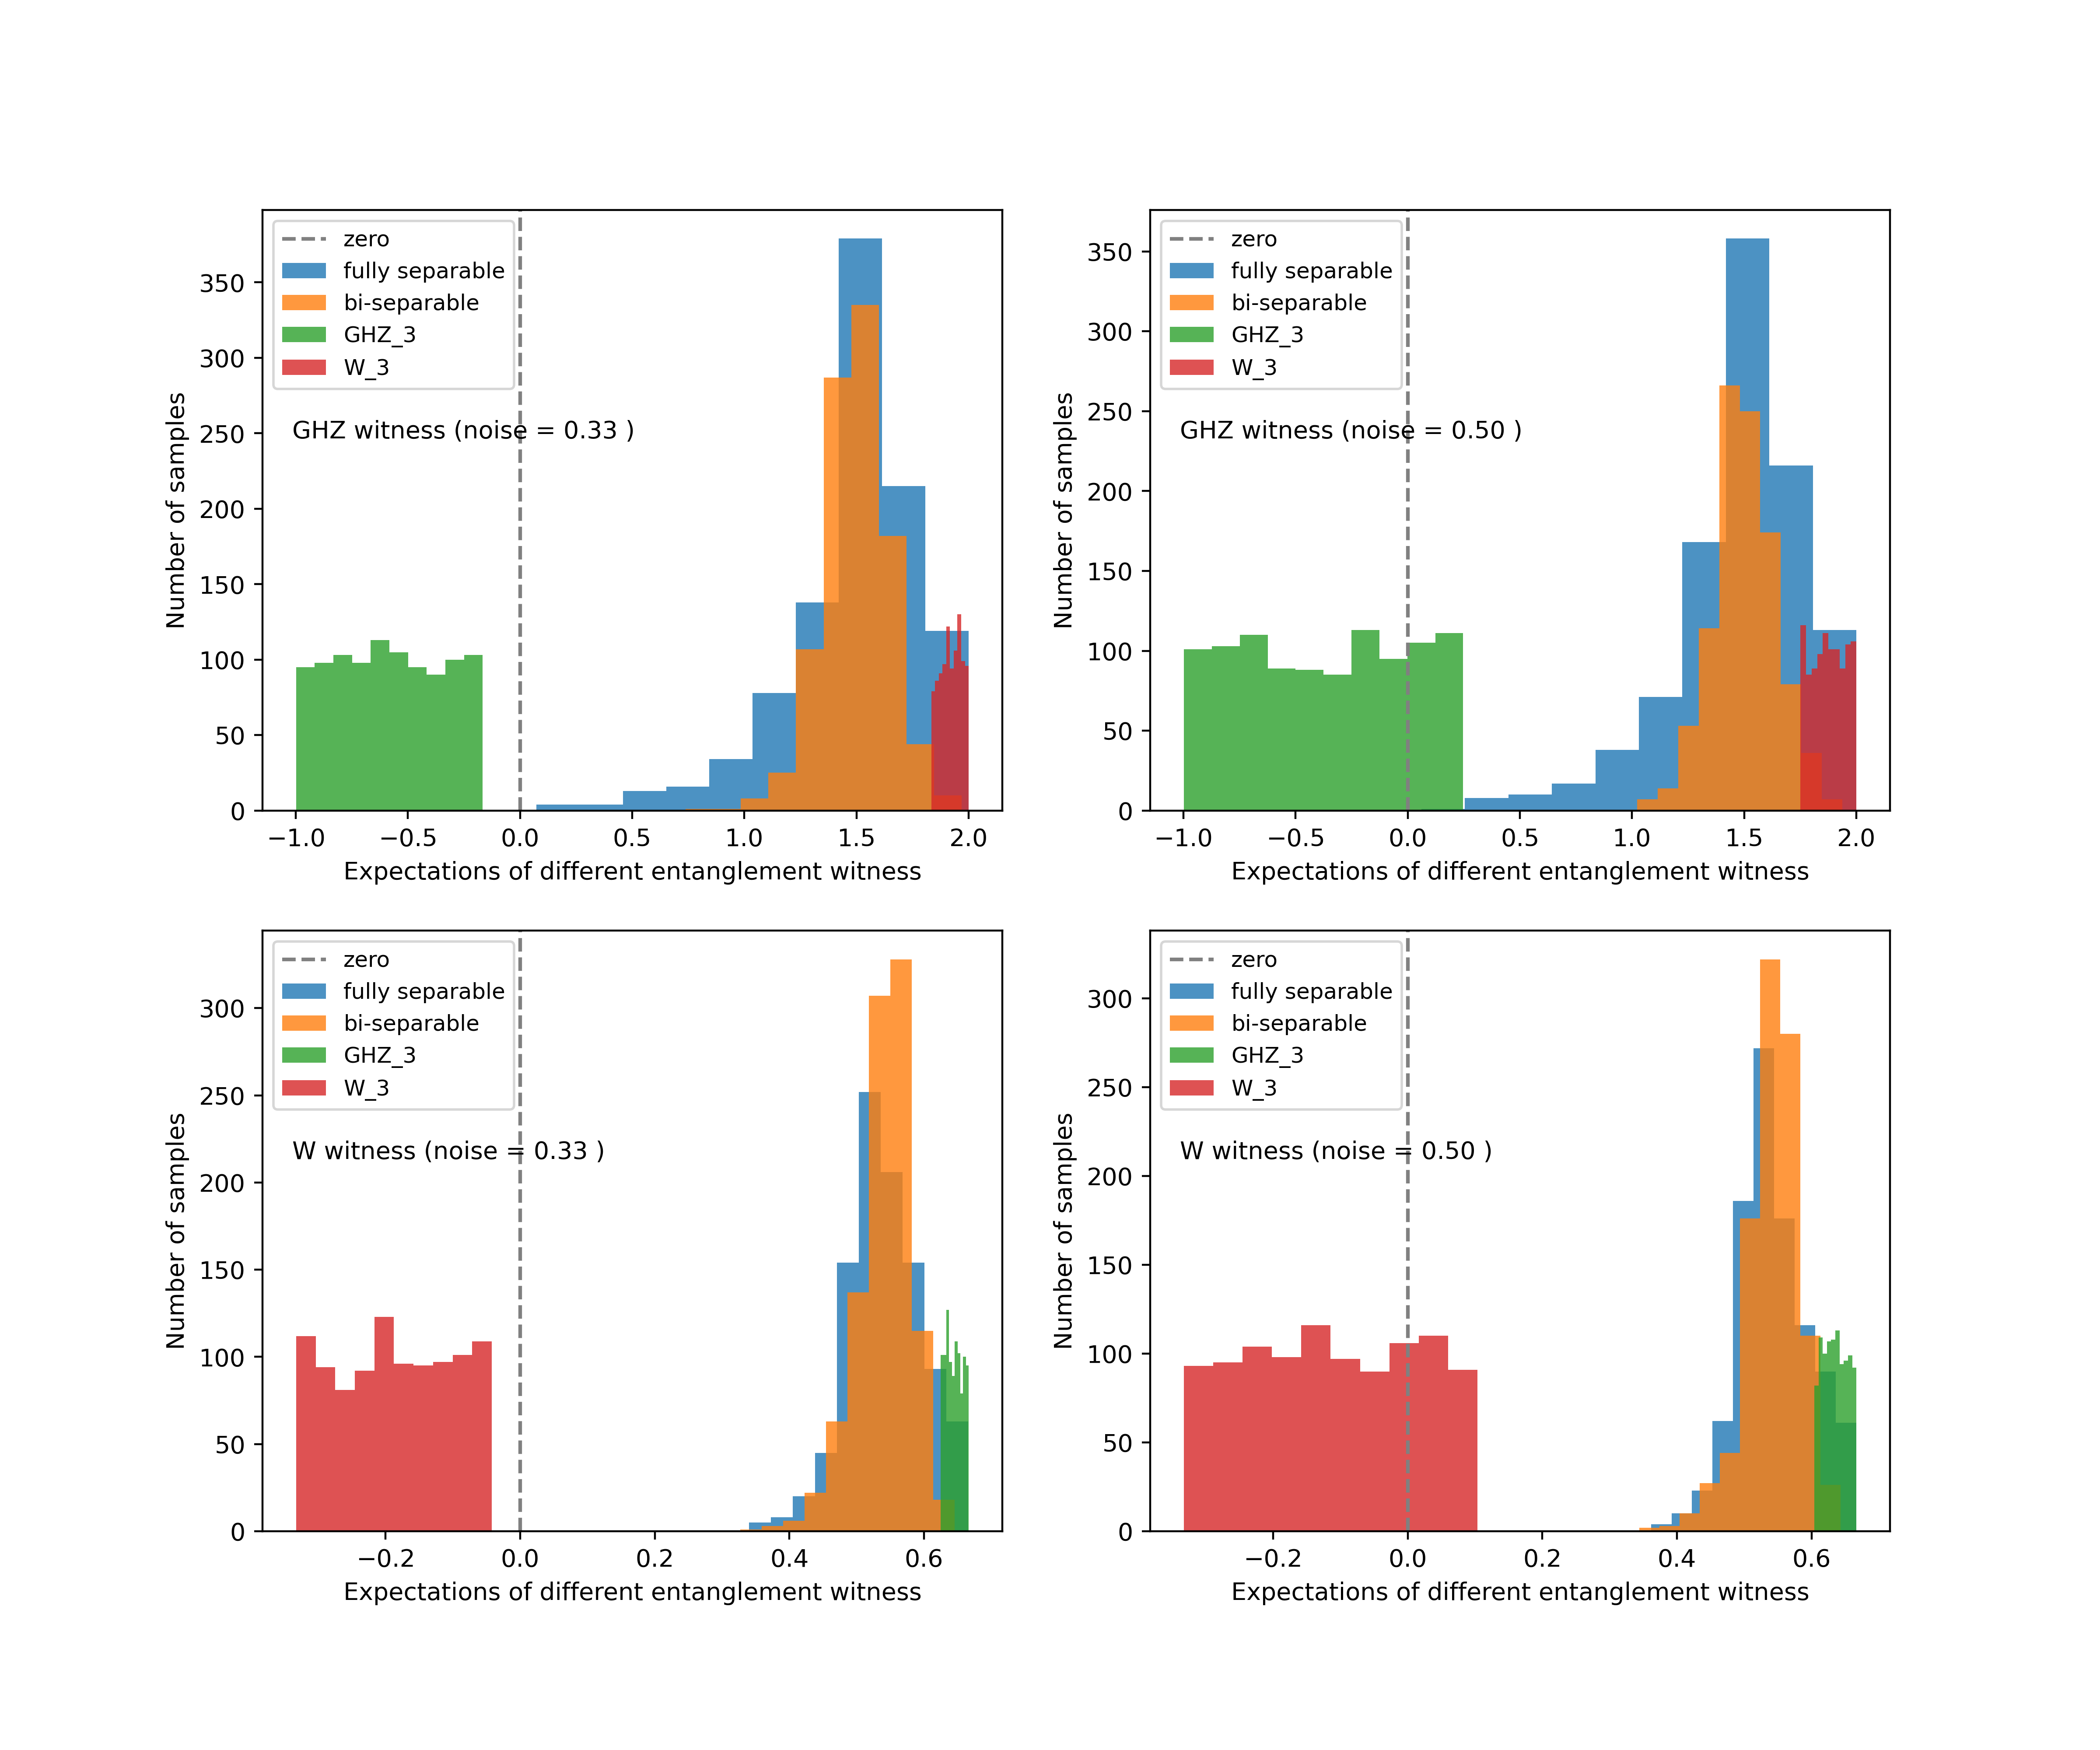
\includegraphics[width=.9\linewidth]{./Code/fidelity_witness_compare.png}
		% 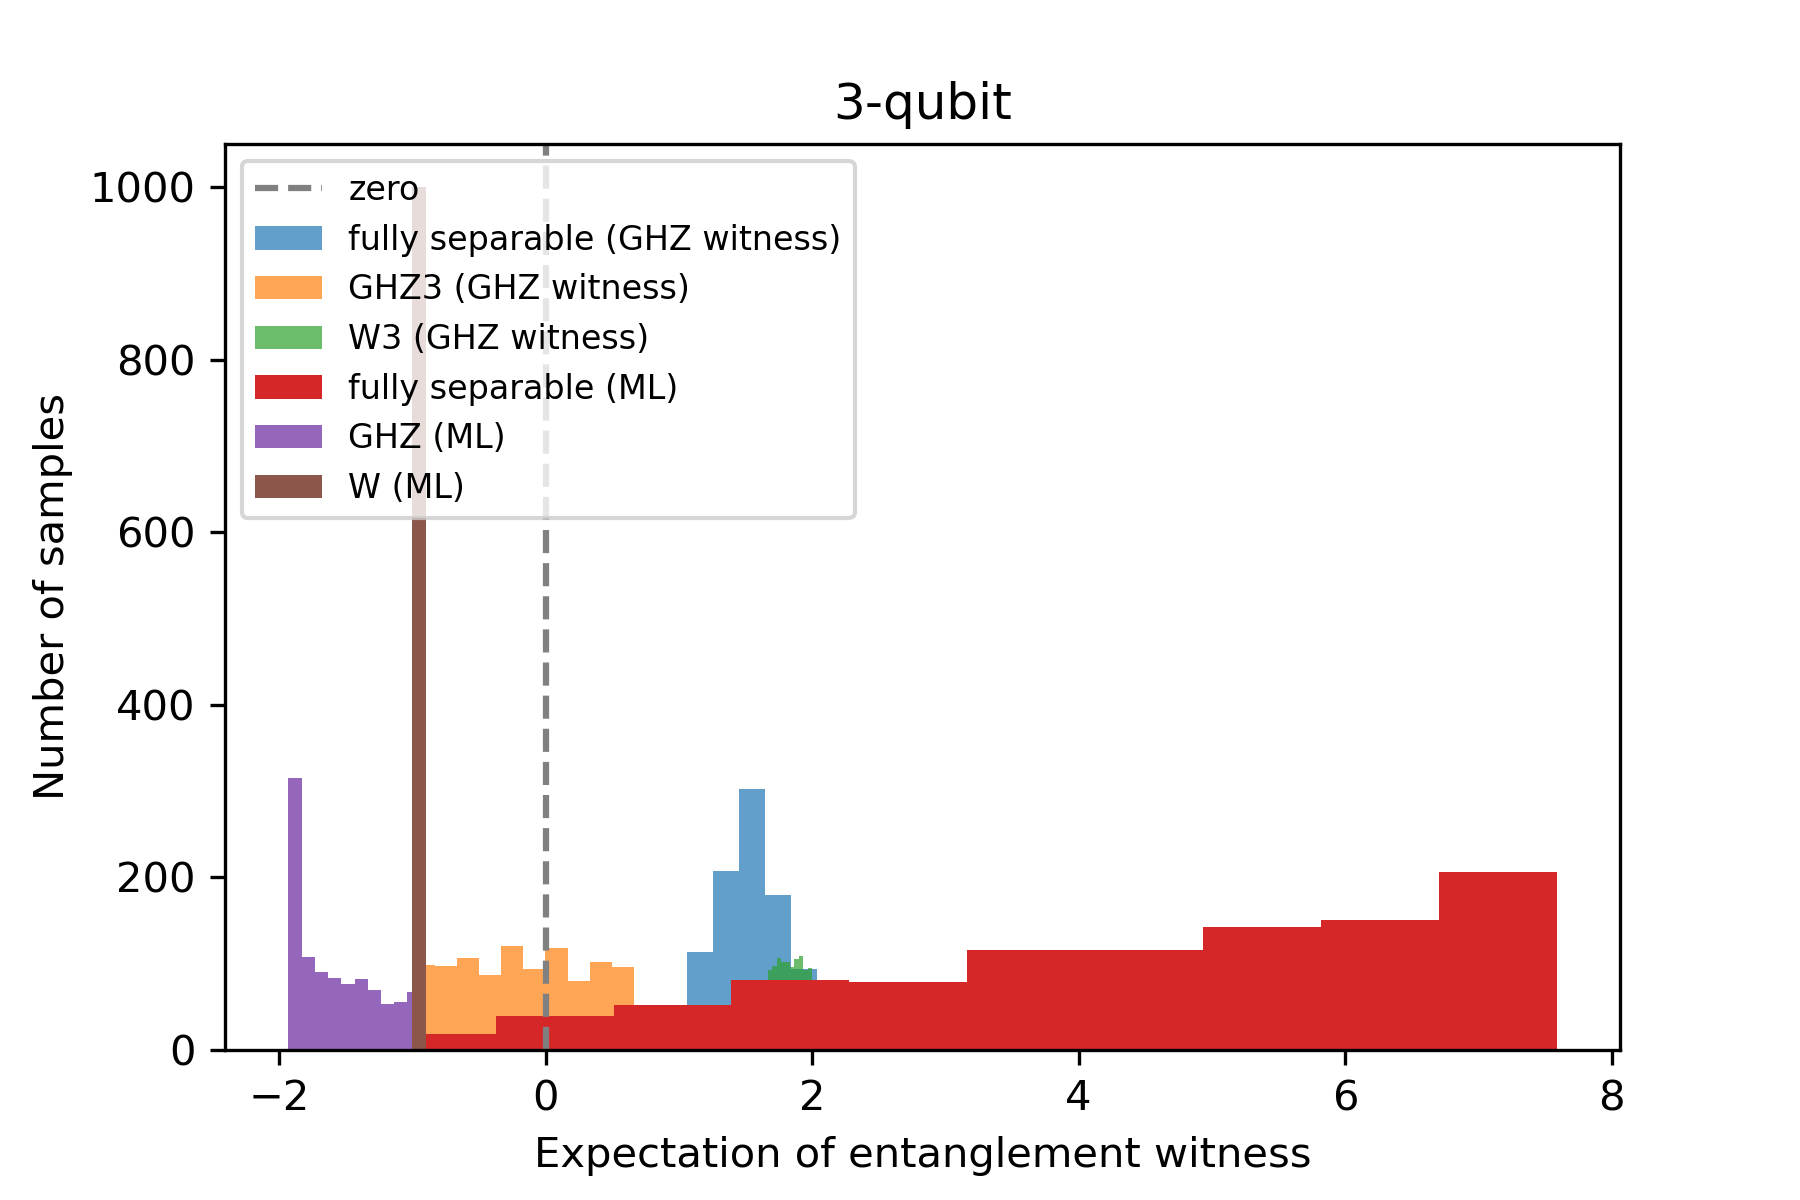
\includegraphics[width=.9\linewidth]{./notebook/three_qubit_hist.png}
		% \caption{ML witness, unfaithful}
	% \end{subfigure}
	% 	\caption{compare different methods: Bell inequality, witness, ML ansatz; different white noise limit, unfaithful state}
	\caption{ML witness for the state cannot be detect by fidelity witness (GHZ state with coherence noise, and W state with large white noise)}
	\label{fig:ml_compare}
\end{figure}

dataset size for training: $10^3$ for 3-qubit case; more qubits [TODO]...
% We consider a set of different regularization parameters,...
\begin{figure}[!ht]
	\centering
	% \includegraphics[width=1\linewidth]{.pdf}
	\caption{[TODO] accuracy VS dataset size, regularization parameters}
\end{figure}


\section{Experiments [TODO]}\label{sec:experiments}
% \subsection{Experiments}
Related experiments: photonic implementation with a few qubits (generation, verification) \cite{luEntanglementStructureEntanglement2018};
fully entangled graph state (ring of 16 qubits) IBM by measuring negativity \cite{wang16qubitIBMUniversal2018};
optical lattice (homogeneous, restricted measurement, detect GME, nonstabilizer) \cite{zhouSchemeCreateVerify2022};
experiments of classical shadow and related comparison \cite{zhangExperimentalQuantumState2021};
detect entanglement by estimating $p_3$-PPT with classical shadow \cite{elbenMixedstateEntanglementLocal2020}.
Similar to the PPT condition, the $p_3$-PPT condition (without full tomography) applies to mixed states and is completely independent of the state in question \cite{elbenMixedstateEntanglementLocal2020}. 
% From this data set, the PT-moments $p_n=\Tr[(\dm_{AB}^{\T_A})^n]$ ($p_2=\Tr[\dm_{AB}^2]$ purity?) can be estimated without having to reconstruct the density matrix $\dm_{AB}$, and with a significantly smaller number of experimental runs $M$ than required for full quantum state tomography.
% c.f. \nameref{thm:multivariate_trace}, 
% \nameref{def:entanglement_spectroscopy}

\section{Conclusion and discussion}
Possible directions for future research:
(1) rigorous proof for dataset size and number of features (required for high training accuracy) scaling with the system size;
(2) better kernel options such as graph kernel, quantum kernel, shadow kernel and neural tangent kernel;
(3) quantum machine learning for estimating all classical features (tomography) efficiently;
(4) if we have all classical features, is it possible to train a universal classifier or with weaker promise;
(5) can we estimate concurrence... by quantum circuit


% \subsection*{Acknowledgements}
\begin{acknowledgments}
\end{acknowledgments}
% \thanks{The author thanks} 
% The author thanks
% TikZiT, QuTip

%\begin{appendices}
    %\chapter{}
%\end{appendices}

% %%%%%%%%%%%%%%%Reference%%%%%%%%%%%%%%%
% % \newpage
% % \printbibliography
\bibliographystyle{apsrev4-2}
%\bibliographystyle{alpha}
\bibliography{ref}

%\begin{widetext}
\onecolumngrid
\appendix

% !TEX root = ./ew.tex


\section{Definitions}\label{sec:definitions}
\begin{definition}[density matrix]\label{def:density_matrix}
	pure state $\ket{\psi}$;
	A quantum state $\dm$ is defined to be a positive operator $ \dm \in \text{End}(V )$ with $\Tr( \dm ) = 1$.
	density matrix $\dm$ (trace one, Hermitian, PSD)...
\end{definition}
\begin{definition}[POVM]\label{def:povm}
	A positive-operator valued measurement (POVM) $M$ consists of a set of positive operators that sum to the identity operator $\identity$. 
	When a measurement $M = \qty{ E_1 , \dots , E_k }$ is applied to a quantum state $\dm$, the outcome is $i \in [k]$ with probability $p_i = \tr( \dm E_i )$.
	observables ... $\expectation[x]\equiv\expval{\ob_x}:=\tr(\ob_x\dm)$
\end{definition}
\begin{definition}[positive, semidefinite]\label{def:psd}
	denoted $X \preceq Y $ provided $Y-X $ is positive
\end{definition}
\begin{definition}[partial trace]\label{def:partial_trace}
	% partial trace;
	reduced density matrix $\dm_A = \Tr_B(\dm_{AB})$
\end{definition}
% \begin{definition}[partial trace]
% 	partial trace
% \end{definition}
\begin{definition}[partial transpose]\label{def:partial_transpose}
	\cite{horodeckiSeparabilityMixedStates1996}
	The partial transpose (PT) operation - acting on subsystem $A$ - is defined as
	\begin{equation}
		\op{k_A,k_B}{l_A,l_B}^{\T_A}
		:= \op{l_A,k_B}{k_A,l_B}
	\end{equation}
	where $\qty{\ket{k_A,k_B}}$ is a product basis of the joint system AB.
\end{definition}
\begin{definition}[maximally entangled]
	a state vector is \emph{maximually entangled} $\iff$ the reduced state at one qubit is maximally mixed, i.e.,
	$\Tr_A(\op{\psi})=\frac{1}{2}$.
\end{definition}
\begin{definition}[entropy]\label{def:entropy}
	In quantum mechanics (information), the von Neumann \emph{entropy} of a density matrix is $H_N(\dm): = -\Tr(\dm \log \dm)=-\sum_i\lambda_i\log(\lambda_i)$;
	In classical information (statistical) theory, the Shannon entropy of a probability distribution $P$ is  $H_S(P):= -\sum_i P(x_i) \log P(x_i)$.
	relative entropy (\nameref{def:divergence})
\end{definition}
\begin{definition}[entanglement entropy]\label{def:entanglement_entropy}
	The bipartite \emph{von Neumann entanglement entropy} $S$
	is defined as the von Neumann entropy of either of
	its reduced density matrix $\dm_A$.
	For a pure state $\dm_{AB}=\op{\Psi}{\Psi}_{AB}$,
	it is given by
	\begin{equation}
		E(\Psi_{AB}) 
		= S(\dm_A)
		= -\Tr(\dm_A \log \dm_A)
		= -\Tr(\dm_B \log \dm_B)
		= S(\dm_B)
	\end{equation}
	where $\dm_A= \Tr_B(\dm_{AB})$ and $\dm_B = \Tr_A(\dm_{AB})$ 
	are the reduced density matrices for each partition.
	With Schmidt decomposition (\cref{eq:schmidt_decomposition}), the entropy of entanglement is simply $-\sum_ip_i^2\log(p_i)$.
	the $n$th Renyi entropy,
	$S_n = \frac{1}{n-1} \log (R_n)$
	% \begin{equation}
	% 	S_n = \frac{1}{n-1} \log (R_n)
	% \end{equation}
	where $R_n = \Tr(\dm^n_A)$
\end{definition}


% \subsubsection{Distance measures}\label{sec:distance_measure}
\begin{definition}[fidelity]\label{def:fidelity}
	Given a pair of states (target $\dm$ and prepared $\dm'$), 
	Uhlmann fidelity $F(\dm,\dm') : = \Tr(\sqrt{\sqrt{\dm}\dm'\sqrt{\dm}})\equiv\norm{\sqrt{\dm}\sqrt{\dm'}}_1$, where $\sqrt{\dm}$ dentoes the positive semidefinite square root of the operator $\dm$. (infidelity $1-F(\dm,\dm')$)
	For any mixed state $\rho$ and pure state $\ket{\psi}$, $F(\dm,\op{\psi})=\sqrt{\mel{\psi}{\dm}{\psi}}\equiv \sqrt{\Tr(\dm\op{\psi})}$ which can be obtained by the Swap-test[?].
	linear fidelity or overlap $F(\dm,\dm'):=\tr(\dm\dm')$.
	% \begin{equation}
	% 	F(\ket{\psi},\ket{\psi'}) :=
	% \end{equation}
	% \begin{equation}
	% 	F(\rho,\rho') : = \Tr \sqrt{\sqrt{\rho}\rho'\sqrt{\rho}}
	% \end{equation}
\end{definition}
different distance measures \cite{badescuQuantumStateCertification2017}
\begin{definition}[norm]\label{def:norm}
	Schatten p-norm $\norm{x}_p:= (\sum_i \abs{x_i}^p)^{1/p}$.
	Euclidean norm $l_2$ norm;
	Spectral (operator) norm $\norm{\vbx}_{\infty}$;
	Trace norm $\norm{A}_{\Tr}\equiv\norm{A}_{1}:=\Tr(\abs{A})\equiv\Tr(\sqrt{A^\dagger A})$, $\abs{A}:=\sqrt{A^\dagger A}$, $p=1$;
	Frobenius norm $\norm{A}_{F}:=\sqrt{\Tr(A^\dagger A)}$, $p=2$;
	Hilbert-Schmidt norm $\norm{A}_{HS}:=\sqrt{\sum_{i,j} A_{ij}^2 }=?\sum_{i\in I}\norm{Ae_i}_H^2$;
	Hilbert-Schmidt inner product $\expval{A,B}_{\textup{HS}}:=\Tr(A^\dagger B)$,
	Frobenius inner product $\expval{A,B}_{\textup{F}}:=\Tr(A^\dagger B)$?
	(in finite-dimensionala Euclidean space, the HS norm is identical to the Frobenius norm)
	Although the Hilbert-Schmidt distance is arguably not too meaningful, operationally, one can use Cauchy-Schwarz to relate it to the very natural trace distance.
\end{definition}
\begin{definition}[distance]\label{def:distance}
	For mixed states, trace distance $d_{\tr}(\dm,\dm') : = \frac{1}{2} \norm{\dm-\dm'}_1$.
	For pure states, $d_{\tr}(\ket{\psi},\ket{\psi'}) : = \frac{1}{2}\norm{\op{\psi} -\op{\psi'}}_1 = \sqrt{1-\abs{\ip{\psi}{\psi'}}^2}$.
	% \begin{equation}
	% 	d_{tr}(\rho,\rho') : = \frac{1}{2} \norm{\rho-\rho'}_1
	% \end{equation}
	fidelity and trace distance are related by the inequalities
	\begin{equation}
		1-F\le D_{\tr}(\dm,\dm') \le \sqrt{1-F^2}
	\end{equation}
	variation distance of two distribution $d_{var}(p,p') : = \frac{1}{2} \sum_i \abs{p_i-p_i'} = \frac{1}{2} \norm{p-p'}_1$.
	% It also has an operational meaning: it is the greatest probability with which one can discriminate a draw from p and a draw from q.
	$l_2$ distance ... Hellinger distance ... HS distance $D_{\text{HS}}(\dm,\dm'): = \norm{\dm-\dm'}_{\text{HS}}=\sqrt{\Tr((\dm-\dm')^2)}$
	% As a probability metric, the $l_2$ distance is somewhat unnatural. For example, it does not satisfy the “data processing inequality”, meaning that there is a stochastic operation that increases $l_2$ distance. However it is by far the easiest distance to calculate, as it is a simple polynomial in p and q; further, it can be related to the total variation distance
\end{definition}


\begin{definition}[input model]\label{def:input_model}
	several common input (encoding) models in quantum algorithms: 
	\begin{itemize}
		% \item qubit (basic) encoding?: given a vector $\vb{z}\in\integer^d$, 
		% $\ket{\vb{z}}=\bigotimes_i^d \ket{\vbx_i}$ where $\vbx_i$ is the binary representation of $z_i$,
		% need $\bigO(d\cdot \log(\max(z_i)))$ (not space efficient)

		% \item phase encoding?

		\item \textbf{amplitude encoding}: given a normalized vector $\vbx\in\realnumber^d$, the quantum state $\ket{\vbx}=\sum_z^d x_z\ket{z}$. 
		need $\log(d) $ qubits for a data point; 
		In general, it is hard to prepare such state. (subject to dequantization \cite{tangQuantumPrincipalComponent2021}). 
		typical encoding method for quantum machine learning for classical problems (such as image classification).
		% qubit (basic) encoding (inefficient? space)

		\item \textbf{unitary encoding}: quantum simulation (Hamiltonian); quantum random walk (adjacency matrix); oracle (controlled) unitary, e.g., quantum phase estimation;
		\nameref{def:graph_state} encoding (discrete, efficient in space/time?, isomorphism?)

		\item \textbf{quantum data}: quantum state $\ket{\psi}$ or $\dm$ from real-world experiments or designed quantum circuits $\U$.
		no input problem? more efficient? for quantum algorithms
		(composed coherently to collect quantum data)

		% \item graph state encoding: \nameref{def:graph_state}, discrete, efficient? space (time), isomorphism?

		% \item (quantum) oracle: $\oracle \ket{i,a}=\ket{i,a+x_i}$; quantum oracle: unitary and controlled unitary
	\end{itemize}
\end{definition}


% \subsection{Stabilizer formalism}\label{sec:stabilizer_formalism}
denote a group by $\group$ and a subgroup $\subgroup$. 
\begin{definition}[Pauli group]
\end{definition}
\begin{definition}[Clifford group]\label{def:clifford}
\end{definition}
\begin{definition}[Stabilizer]\label{def:stabilizer}
	An observable $S_k$ is a stabilizing operator of an $n$-qubit state $\ket{\psi}$ if the state $\ket{\psi}$ is an eigenstate of $S_k$ with eigenvalue 1,

	A stabilizer set $S = \qty{ S_1, \dots , S_n}$ consisting of n mutually commuting and independent stabilizer operators is called the set of stabilizer “generators”.
\end{definition}
Many highly entangled $n$-qubit states can be uniquely defined by $n$ stabilizing operators which are locally measurable, i.e., they are products of Pauli matrices.
A stabilizer $S_i$ is an n-fold tensor product of $n$ operators chosen from the one qubit Pauli operators $\qty{\identity,X,Y,Z}$.

\section{Machine learning background}
% As these areas are extremely broad, we cannot completely review all known literature; we will simply give pointers to some of the best known and most relevant results.

% In this work, we restrict ourself to supervised learning (mainly SVM), where we are given a set of labeled data for training to predict labels of new data.

Notations:
The (classical) training data (for supervised learning) is a set of $m$ data points $\qty{(\vbx^{(i)}, y^{(i)})}^{m}_{i=1}$ 
where each data point is a pair $(\vbx,y)$.
Normally, the input (e.g., an image) $\vbx:= (x_1,x_2,\dots,x_d) \in \realnumber^d$  is a vector where $d$ is the number of \emph{features}
and its \emph{label} $y\in\Sigma$ is a scalar with some discrete set $\Sigma$ of alphabet/categories. 
For simplicity and the purpose of this paper, we assume $\Sigma=\qty{-1,1}$ (binary classification).


\subsection{Support vector machine}\label{sec:svm}
SVM is a typical supervised learning algorithm for classification. Taking the example of classifying cat/dog images, supervised learning means we are given a dataset in which every image is labeled either a cat or a dog such that we can find a function classifying new images with high accuracy. More precisely,  the training dataset is a set of pairs of features X and their labels y. In the image classification case, features are obtained by transforming all pixels of an image into a vector. In SVM, we want to find a linear function, that is a hyperplane which separates cat data from dog data. So, the prediction label is given by the sign of the inner product (projection) of the hyperplane and the feature vector. We can observe that the problem setting of image classification by SVM is quite analogous to entanglement detection, where input data are quantum states now and the labels are either entangled or separable.


\begin{definition}[SVM]\label{def:svm}
	Given a set of (binary) labeled data,
	support vector machine (SVM) is designed to
	find a hyperplane (a linear function) such that maximize the margin between two partitions...
	\begin{equation}
		\max_{\vb{w}} 
		....
	\end{equation}
\end{definition}

\subsubsection{kernel method}
However, note that SVM is only a linear classifier. while most real-world data, such as cat/dog images and entangled/separable quantum states are not linearly separable. For example, with this two dimension dataset, we are unable to find a hyperplane to separate red points from the purple points very well. Fortunately, there is a very useful tool called kernel method or kernel trick to remedy this drawback. The main idea is mapping the features to a higher dimensional space such that  they can be linearly separated in the high dimensional feature space. Just like this example, two dimensional data are mapped to the three dimensional space. Now, we can easily find the separating plane. With SVM and kernel methods, we expect to find a generic and flexible way for entanglement detection.
\nameref{def:kernel}
\begin{definition}[kernel]\label{def:kernel}
	In general, the kernel function $\kernel:\mathcal{X}\times \mathcal{X} \to \realnumber$ measures the similarity between two input data points by an inner product
	\begin{equation}
		\kernel (\vbx,\vbx') : = \expval{\phi(\vbx),\phi(\vbx')}
	\end{equation}
	If the input $\vbx\in \realnumber^d$ (conventional machine learning task, e.g., image classification), the feature map $\phi(\vbx): \realnumber^d\to \realnumber^n$ ($d < n$) from a low dimensional space to a higher dimensional space.
	The corresponding kernel (Gram) matrix $\mathbf{K}$ should be a positive, semidefinite (PSD) matrix, i.e. all eigenvalues are non-negative
\end{definition}
\begin{example}[kernels]
	Some common kernels: 
	the polynomial kernel $\kernel_{\text{poly}}(\vbx,\vbx') := (1+\vbx\cdot\vbx')^q$ with feature map $\phi(\vbx)$ ...
	The Gaussian kernel
	$\kernel_{\text{gaus}}(\vbx,\vbx') := \exp(-\gamma\norm{\vbx-\vbx'}^2_2)$ 
		% \begin{equation}
		% 	\kernel_{\text{gaus}}(\vbx,\vbx') := \exp(-\norm{\vbx-\vbx'}^2/(2\beta))
		% \end{equation}
	with an infinite dimensional feature map $\phi(\vbx)$.
	An important feature of kernel method is that kernels can be computed efficiently without evaluating feature map (might be infinite dimension) explicitly.
	% \begin{itemize}
	% 	\item \emph{Gaussian kernel}; 
	% 	\begin{equation}
	% 		\kernel_{\text{gaus}}(\vbx,\vbx') := \exp(-\norm{\vbx-\vbx'}^2/(2\beta))
	% 	\end{equation}
	% 	note that infinite dimensional feature map

		% \item \emph{graph kernel} \cite{kriegeSurveyGraphKernels2020}: given a pair of graphs $(\graph,\graph')$
		% \begin{equation}
		% 	\kernel (\graph,\graph')  =
		% \end{equation}
		% quantum graph kernel $\kernel (\graph,\graph')  = \abs{\ip{\graph}{\graph'}}^2$ ??
		% \cite{baiQuantumJensenShannon2015}

		% \item quantum kernel (transition amplitude / quantum propagator);
		% \begin{equation}
		% 	k_Q(\rho,\rho') := \abs{\ip{\phi(x)}{\phi(x')}}^2 =\abs{\mel{0}{\U_{\phi(x)}^\dagger \U_{\phi(x')} }{0}}^2 = \Tr(\rho\rho')
		% \end{equation}
		% with quantum feature map $\phi(x): \mathcal{X}\to \op{\phi(x)}$

		% \item \emph{shadow kernel}:
		% given two density matrices $\rho$ and $\rho'$
		% \begin{equation}
		% 	k_{\shadow}(\rho,\rho') := 
		% \end{equation}

	% 	\item neural tagent kernel \cite{jacotNeuralTangentKernel2020}: proved to be equivalent to deep neural network \cite{gaoEfficientRepresentationQuantum2017}
	% \end{itemize}
\end{example}

similarity measures? advantages? why? (isomorphism?)
\begin{definition}[divergence]\label{def:divergence}
	KL divergence (relative \nameref{def:entropy}): measure the distance (similarity) between two probability distributions:
	\begin{equation}
		\kl (P || Q) := \sum P(x) \log (P(x)/Q(x))
	\end{equation}
	symmetric version: Jensen-Shannon divergence (machine learning)
	\begin{equation}
		\jsd (P || P') := \frac{1}{2} \qty(\kl(P|| M) + \kl(P'||M))
		\equiv H_S(M)-\frac{1}{2} (H_S(P) - H_S(P') ) 
	\end{equation}
	where $M=(P+P')/2$ and Shannon \nameref{def:entropy} $H_S$.
	Analogously, quantum Jensen-Shannon divergence $D_{\qjs}$ of two density matrices can be defined...
	\begin{equation}
		D_{\qjs}(\dm||\dm'):= 
		H_V(\dm_M) - \frac{1}{2} (H_V(\dm) - H_V(\dm') ) 
	\end{equation}
	as a quantum graph kernel ($\dm$ induced by quantum random walk)
\end{definition}
\begin{definition}[geometric difference]\label{def:geometric_difference}
	\begin{equation}
		g(K^1|| k^2) = \sqrt{\norm{\sqrt{K^2} (K^1)^{-1}\sqrt{K^2}}_{\infty}}
	\end{equation}
	where $\norm{\cdot}_{\infty}$ is the spectral \nameref{def:norm}.
\end{definition}

\subsubsection{Graph kernel}
\begin{definition}[graph property]\label{def:graph_property}
	% The setting of graph property testing provides a natural class of partial graph properties.
	monotone ...
\end{definition}
\begin{example}[colorable]\label{exm:colorable}
	$k$-colorable is a graph property, i.e., allow for a coloring of the vertices with $k$ colors such that no two adjacent vertices have the same color.
	A graph is bipartite $\iff$ 2-colorable.
	other graph properties: isomorphism; vertex cover; Hamiltonian cycle ...
\end{example}
\begin{problem}[graph property test]\label{prm:graph_property_test}
	\textbf{promise}: the input graph either has a property, or is $\epsilon$-far from having the property, meaning that we must change at least an $\epsilon$ fraction of the edges to make the property hold.
\end{problem}
\begin{theorem}[bounds for graph property test]
\end{theorem}
\begin{question}
	\cite{montanaroSurveyQuantumProperty2018}
	Is there any graph property which admits an exponential quantum speed-up?
	\cite{ben-davidSymmetriesGraphProperties2020}
	depends on input model (query adjacency matrix/list)
	% quantum algorithms (bounds) for graph properties \cite{ben-davidSymmetriesGraphProperties2020}
\end{question}
Graphs is another kind of data which is fundamentally different from a real value vector because of vertex-edge relation and graph isomorphism.
So, graph kernel \cite{kriegeSurveyGraphKernels2020} need additional attention.
\begin{definition}[graph kernel]\label{def:graph_kernel}
	given a pair of graphs $(\graph,\graph')$,
	\emph{graph kernel} is $\kernel (\graph,\graph')  =$.
	% \begin{equation}
	% \end{equation}
	quantum graph kernel $\kernel (\graph,\graph')  = \abs{\ip{\graph}{\graph'}}^2$ ??
	\cite{baiQuantumJensenShannon2015}	
\end{definition}

\subsubsection{Quantum kernel}
related works:
\begin{itemize}
	\item quantum kernel method: estimate kernels by quantum algorithms (circuits)	\cite{havlicekSupervisedLearningQuantum2019}
	\cite{schuldQuantumMachineLearning2019}: for classical problem (data)

	\item rigorous and robust quantum advantage of quantum kernel method in SVM \cite{liuRigorousRobustQuantum2021}. group structured data \cite{glickCovariantQuantumKernels2021}

	\item power of data in quantum machine learning \cite{huangPowerDataQuantum2021}: input??? projected quantum kernel
\end{itemize}
\begin{definition}[quantum kernel]\label{def:quantum_kernel}
	quantum kernel 
	with quantum feature map $\phi(\vbx): \mathcal{X}\to \op{\phi(\vbx)}$
	\begin{equation}
		k_Q(\rho,\rho') := \abs{\ip{\phi(\vbx)}{\phi(\vbx')}}^2 =\abs{\mel{0}{\U_{\phi(\vbx)}^\dagger \U_{\phi(\vbx')} }{0}}^2 =? \Tr(\rho\rho') \equiv \expval{\dm,\dm'}_{\textup{HS}}
	\end{equation}
	where $\U_{\phi(\vbx)}$ is a quantum circuit or physics process that encoding an input $\vbx$.
	In quantum physics, quantum kernel is also known as transition amplitude (quantum propagator);
\end{definition}
% \begin{definition}[multivariate trace estimation]\label{def:multivariate_trace_estimation}
% 	The task of estimating quantities like 
% 	\begin{equation}
% 		\Tr(\rho_1 \cdots \rho_m)
% 		\tag{multivariate traces}
% 	\end{equation}
% 	given access to copies of the quantum states $\rho_1$  through $\rho_m$.
% \end{definition}
% is a fundamental building block in quantum information science

% power of data - 
\begin{proposition}[\cite{huangPowerDataQuantum2021}]
	If a classical algorithm without training data can compute (label) $y=f(x)=\mel{x}{\U_{\textup{QNN}}^\dagger \ob U_{\textup{QNN}}}{x}$ (with amplitude encoding) efficiently (poly time in ...) for any $\U_{\textup{QNN}}$ and $\ob$, then $\nameref{def:bpp}=\nameref{def:bqp}$ (which is believed unlikely).
\end{proposition}
\begin{proposition}[\cite{huangPowerDataQuantum2021}]
	Training an arbitrarily deep quantum neural network $\U_{\qnn}$ with a trainable observable $\ob$ is equivalent to training a \nameref{def:quantum_kernel} method with kernel $k_{Q}(\vbx,\vbx')=\Tr(\dm(\vbx)\dm'(\vbx'))$
\end{proposition}
\begin{definition}[projected quantum kernel]\label{def:projected_quantum_kernel}
	....
\end{definition}


\subsection{Neural network}\label{sec:neural_network}
\subsubsection{neural network and kernel}
\begin{definition}[neural tagent kernel]\label{def:neural_tangent_kernel}
	neural tangent kernel \cite{jacotNeuralTangentKernel2020}: proved to be equivalent to deep neural network \cite{gaoEfficientRepresentationQuantum2017} in the limit ...
	\begin{equation}
		k_{\ntk} \qty(S_T(\dm_l),\tilde{S}_T(\dm_{l'}))
		=
		\expval{
			\phi^{(\ntk)}(S_T(\dm_l)),
			\phi^{(\ntk)}(\tilde{S}_T(\dm_l))
		}
	\end{equation}
\end{definition}



\subsubsection{quantum neural network}\label{sec:quantum_neural_network}
% \subsection{Unsupervised: PCA}

\section{Hardness assumptions}
\begin{definition}[\NP]\label{def:np}
	\NP, \NP-hard, \NP-complete
\end{definition}
\begin{definition}[\sharpP]\label{def:sharpp}
	\sharpP
\end{definition}
\begin{definition}[QMA]\label{def:qma}
	QMA
\end{definition}
\begin{definition}[\BPP]\label{def:bpp}
	\BPP
\end{definition}
\begin{definition}[\BQP]\label{def:bqp}
	\BQP
\end{definition}

%\end{widetext}

\end{document}